\chapter{极性锑化铟的生长机理研究}
\section{引言}
III-V族化合物半导体被认为是下一代电子器件和光电子器件有利的材料候选。以III-V族化合物半导体\cemb{InSb}为例,块体状态的\cemb{InSb}具有较小的带隙和极高的电子迁移能力\citing{RN919-2019, RN897-1984, RN898-2020}。当结构尺度减小至低维,\cemb{InSb}展现出了更多新颖的物理特性,如非常强的自旋-轨道作用\citing{RN887-2021, RN922-2010, RN924-2015},较大的朗德g(Landé g-factor)因子\citing{RN925-2008}以及二维电子气等\citing{RN899-2020, RN926-2021}。这些新颖的物理特性使得低维\cemb{InSb}纳米结构可以用于自旋电子\citing{RN927-2017, RN928-2020},拓扑量子计算等量子器件的构建\citing{RN946-2017, RN737-2015, RN921-2016, RN933-2015}。同时,III-V族化合物半导体的单层化也有研究者进行了稳定性以及电子特性研究\citing{RN918-2013}。

在\ref{cap:石墨烯的生长机理研究}中,我们计算了石墨烯在化学气相沉积环境下的生长机理。以石墨烯为代表的单元素平面二维材料,在理想的晶格状态下所有原子都处于同一平面,具有平面外方向的镜面对称性和反演对称性\citing{RN664-2017, RN903-2021}。而对于晶格结构以闪锌矿(zinc blende,ZB)和纤锌矿(wurtzite,WZ)为主的III-V族化合物半导体,其晶格对称性决定了在<111>晶向缺少反演对称。反演对称性的破缺使得III-V族化合物半导体的(111)晶面具有两个不同的端面,即以III族元素为端点的III极性和以V族元素为端点的V极性。不同极性表面原子的不同导致了III-V化合物半导体不同极性的(111)面表现出不同的物理化学特性\citing{RN910-2004}。III-V化合物半导体的表面极性同时也对生长过程中的III-V化合物的生长机理以及生长形貌产生影响\citing{RN929-2015, RN916-2018}。先前的研究表明,\cemb{InSb(111)}表面的许多新奇的物理现象与所处的极性息息相关。例如在特定极性的\cemb{InSb(111)}表面可以异质外延生长具有优异电子性质的新型材料 \citing{RN902-2016, RN852-2021, RN901-2019, RN900-2017, RN891-2019}。

分子束外延(molecular beam epitaxy,MBE)技术以及各种高级材料观测技术(如球差矫正透射电子显微镜)的发展使得研究者能够进一步研究III-V化合物半导体生长过程中极性的演化及调控手段。1994年,研究者发现在\cemb{InSb/Sn/InSb}异质结构中,底端\cemb{InSb}的极性可以透过5原子层的\cemb{Sn}薄膜,对上层的\cemb{InSb}的极性产生影响。随后的研究发现,大多数的III-V化合物半导体倾向于生长V极性的纳米结构\citing{RN864-2019, RN930-1998, RN931-2010},通过不同的生长手段,也有研究者生长出了III极性的表面\citing{RN930-1998, RN931-2010}。通过对实验参数和生长环境进行细致的控制,研究者能够利用分子束外延的方法对所合成的III-V化合物半导体纳米结构进行生长极性控制 \citing{RN913-2016, RN858-2019, RN889-2011, RN911-2019}。得益于合成技术的发展,研究者对于III-V半导体的生长机制进行了大量的实验观测和理论探究,力图对其中的极性演化规律产生更深的理解,从而能够更好的对III-V化合物半导体低维纳米结构进行定极性生长\citing{RN878-2020, RN940-1979, RN936-2002, RN886-2021, RN932-2018, RN894-2012, RN934-2018, RN941-2016}。

在本章中,以III-V族化合物半导体\cemb{InSb}为例,我们系统的探究了双层\cemb{InSb(111)}在\cemb{Bi(001)}衬底上的生长序列以及形貌演化规律。我们的研究表明在\cemb{Bi}衬底上,\cemb{InSb}的极化从第二层生长开始。单层的\cemb{InSb}在在\cemb{Bi}衬底上表现出非晶的形态。我们绘制了双层\cemb{InSb}在
\cemb{Bi}衬底上的极化相图,并且探究了从单层到双层\cemb{InSb}表面极性变化的物理成因。
\section{计算细节}
在本章中,密度泛函理论主要使用Vienna ab-initio Simulation Package (VASP) 软件包进行计算\citing{RN681-1996, RN682-1996}。在密度泛函理论计算中,我们使用广义梯度近似(GGA)下的Perdew-Burke-Ernzerhof (PBE)泛函描述电子之间的交换关联作用\citing{RN683-1996}。平面波的截断动能取为为$\SI{500}{\electronvolt}$。\cemb{InSb(111)}与衬底\cemb{Bi(001)}之间的范德瓦尔斯作用使用Grimme的DFT-D3方法进行描述,并带有Becke-Johnson阻尼作用 \citing{RN937-2010, RN938-2011}。对于$1 \times 1$和$2 \times 2$大小的切片模型,我们使用以$\Gamma$ 点为中心的$11 \times 11 \times 1$和$7 \times 7 \times 1$的K空间采样网络进行布里渊区积分。而对于实空间体积更大的切片模型以及团簇模型,我们仅对$\Gamma$ 点进行采样。在原子结构优化的计算中,力收敛条件设为$\SI{1e-2}{\electronvolt \per \angstrom}$,电子结构自洽场计算的收敛条件设为$\SI{1e-6}{\electronvolt}$。对于过渡态的计算,我们采用CI-NEB(Climbing Image Nudged Elastic Band)方法对始末反应状态之间的能量鞍点进行搜寻,以确定反应势垒的大小\citing{RN790-2000}。对于过渡态计算,力收敛条件设为$\SI{3e-2}{\electronvolt \per \angstrom}$。

对于极性面的表面能,我们使用赝氢饱和法及四面体法进行计算\citing{RN300-2016}。用于表面能计算的\cemb{InSb}切片模型以及四面体模型均基于优化过的块体\cemb{InSb},并进行了进一步的结构优化。计算表面能的切片模型的大小为$2 \times 2$,包含至少9层\cemb{InSb(111)}双原子层。对于\cemb{InSb(111)/Bi(001)}体系,我们是由六层\cemb{Bi(001)}双原子层作为衬底。衬底底面原子在优化过程中固定在块体构型,用以模拟半无限衬底。在\cemb{Bi(001)}表面,\cemb{InSb(111)}覆盖层的晶格由于约$\SI{1.9}{\percent}$等晶格失配而有微小的形变。切片模型的垂直表面方向放置至少$\SI{20}{\angstrom}$的真空层以防止周期性条件相邻切片的影响。在我们的计算中,块体\cemb{InSb}和块体\cemb{Bi}的晶格常数分别为\SI{6.62}{\angstrom}和\SI{4.79}{\angstrom},与先前文献报道一致\citing{RN939-2013,RN1266-1965}。

为了估计原子之间的作用强弱,我们使用LOBSTER软件包对晶体轨道哈密顿量布居(Crystal Orbital Hamilton Population, COHP)进行了计算和分析\citing{RN951-2011, RN950-1993, RN949-2016}。在本章中,\cemb{InSb(111)/Bi(001)}体系中的成键强弱由-COHP谱和-COHP积分(-ICOHP)进行量化。-ICOHP由-COHP谱中的电子占据态积分而来。在-COHP和-ICOHP中,成键态以正值表示,反键态以负值表示。
\section{单层锑化铟的生长机理}

\subsection{\cemb{Bi(001)}衬底表面锑、铟原子的吸附机理}
\def\TfourSite{\rm T_{4} \it}
\def\HthreeSite{\rm H_{3} \it}
对于\cemb{InSb(111)}极性面在\cemb{Bi(001)}衬底表面的生长机理,我们首先对衬底表面锑、铟原子的吸附进行研究。在衬底表面,吸附原子的结合能$\energyVar{b}{}$为\chinesecolon
\[
    \energyVar{b}{}=\left(\energyVar{sub+adatom}{}-\energyVar{sub}{}-N\muVar{adatom}{}\right)/ N
\]

其中,$\energyVar{sub+adatom}{}$和$\energyVar{sub}{}$为吸附有原子的衬底和未吸附原子的衬底的能量。$\muVar{adatom}{}$为吸附原子的化学势。$N$为吸附原子的总数。

我们考虑\cemb{In}和\cemb{Sb}吸附原子在\cemb{Bi(001)}表面吸附覆盖率为$1/ 4$的结合能,计算结果如\ref{fig:IS_Bi_adatoms}所示。根据我们的计算,\cemb{In}原子和\cemb{Sb}原子都更倾向于吸附在\cemb{Bi(001)}衬底表面的$\TfourSite$位和$\HthreeSite$位。如图\ref{fig:IS_structure_T4onBi}和\ref{fig:IS_structure_H3onBi}所示,$\TfourSite$为\cemb{Bi(001)}衬底表面的四重配位顶位,正对于第一层\cemb{Bi}双原子层的下层原子。$HthreeSite$为\cemb{Bi(001)}衬底表面的三种配位空心位,正对于第一层\cemb{Bi}双原子层的空心以及第二层\cemb{Bi}双原子层的上层原子。\cemb{In}原子和\cemb{Sb}原子在\cemb{Bi(001)}衬底表面的吸附能如图\ref{fig:IS_DFT_adatomBind}所示,计算表明\cemb{Bi(001)}衬底表面的$\TfourSite$为\cemb{In}原子和\cemb{Sb}原子的最佳吸附位点。而$\HthreeSite$为二者的次优吸附位点。在吸附能以及后续的能量计算中,我们使用\cemb{In}的化学势$\muVar{In}{}$来表示\cemb{In}元素在生长气氛中的活性水平,体现在\cemb{InSb}化学平衡下\cemb{In}元素和\cemb{Sb}元素的浓度差距。

\begin{figure}[htb]
    \subfloat[]{
        \label{fig:IS_DFT_adatomBind}
        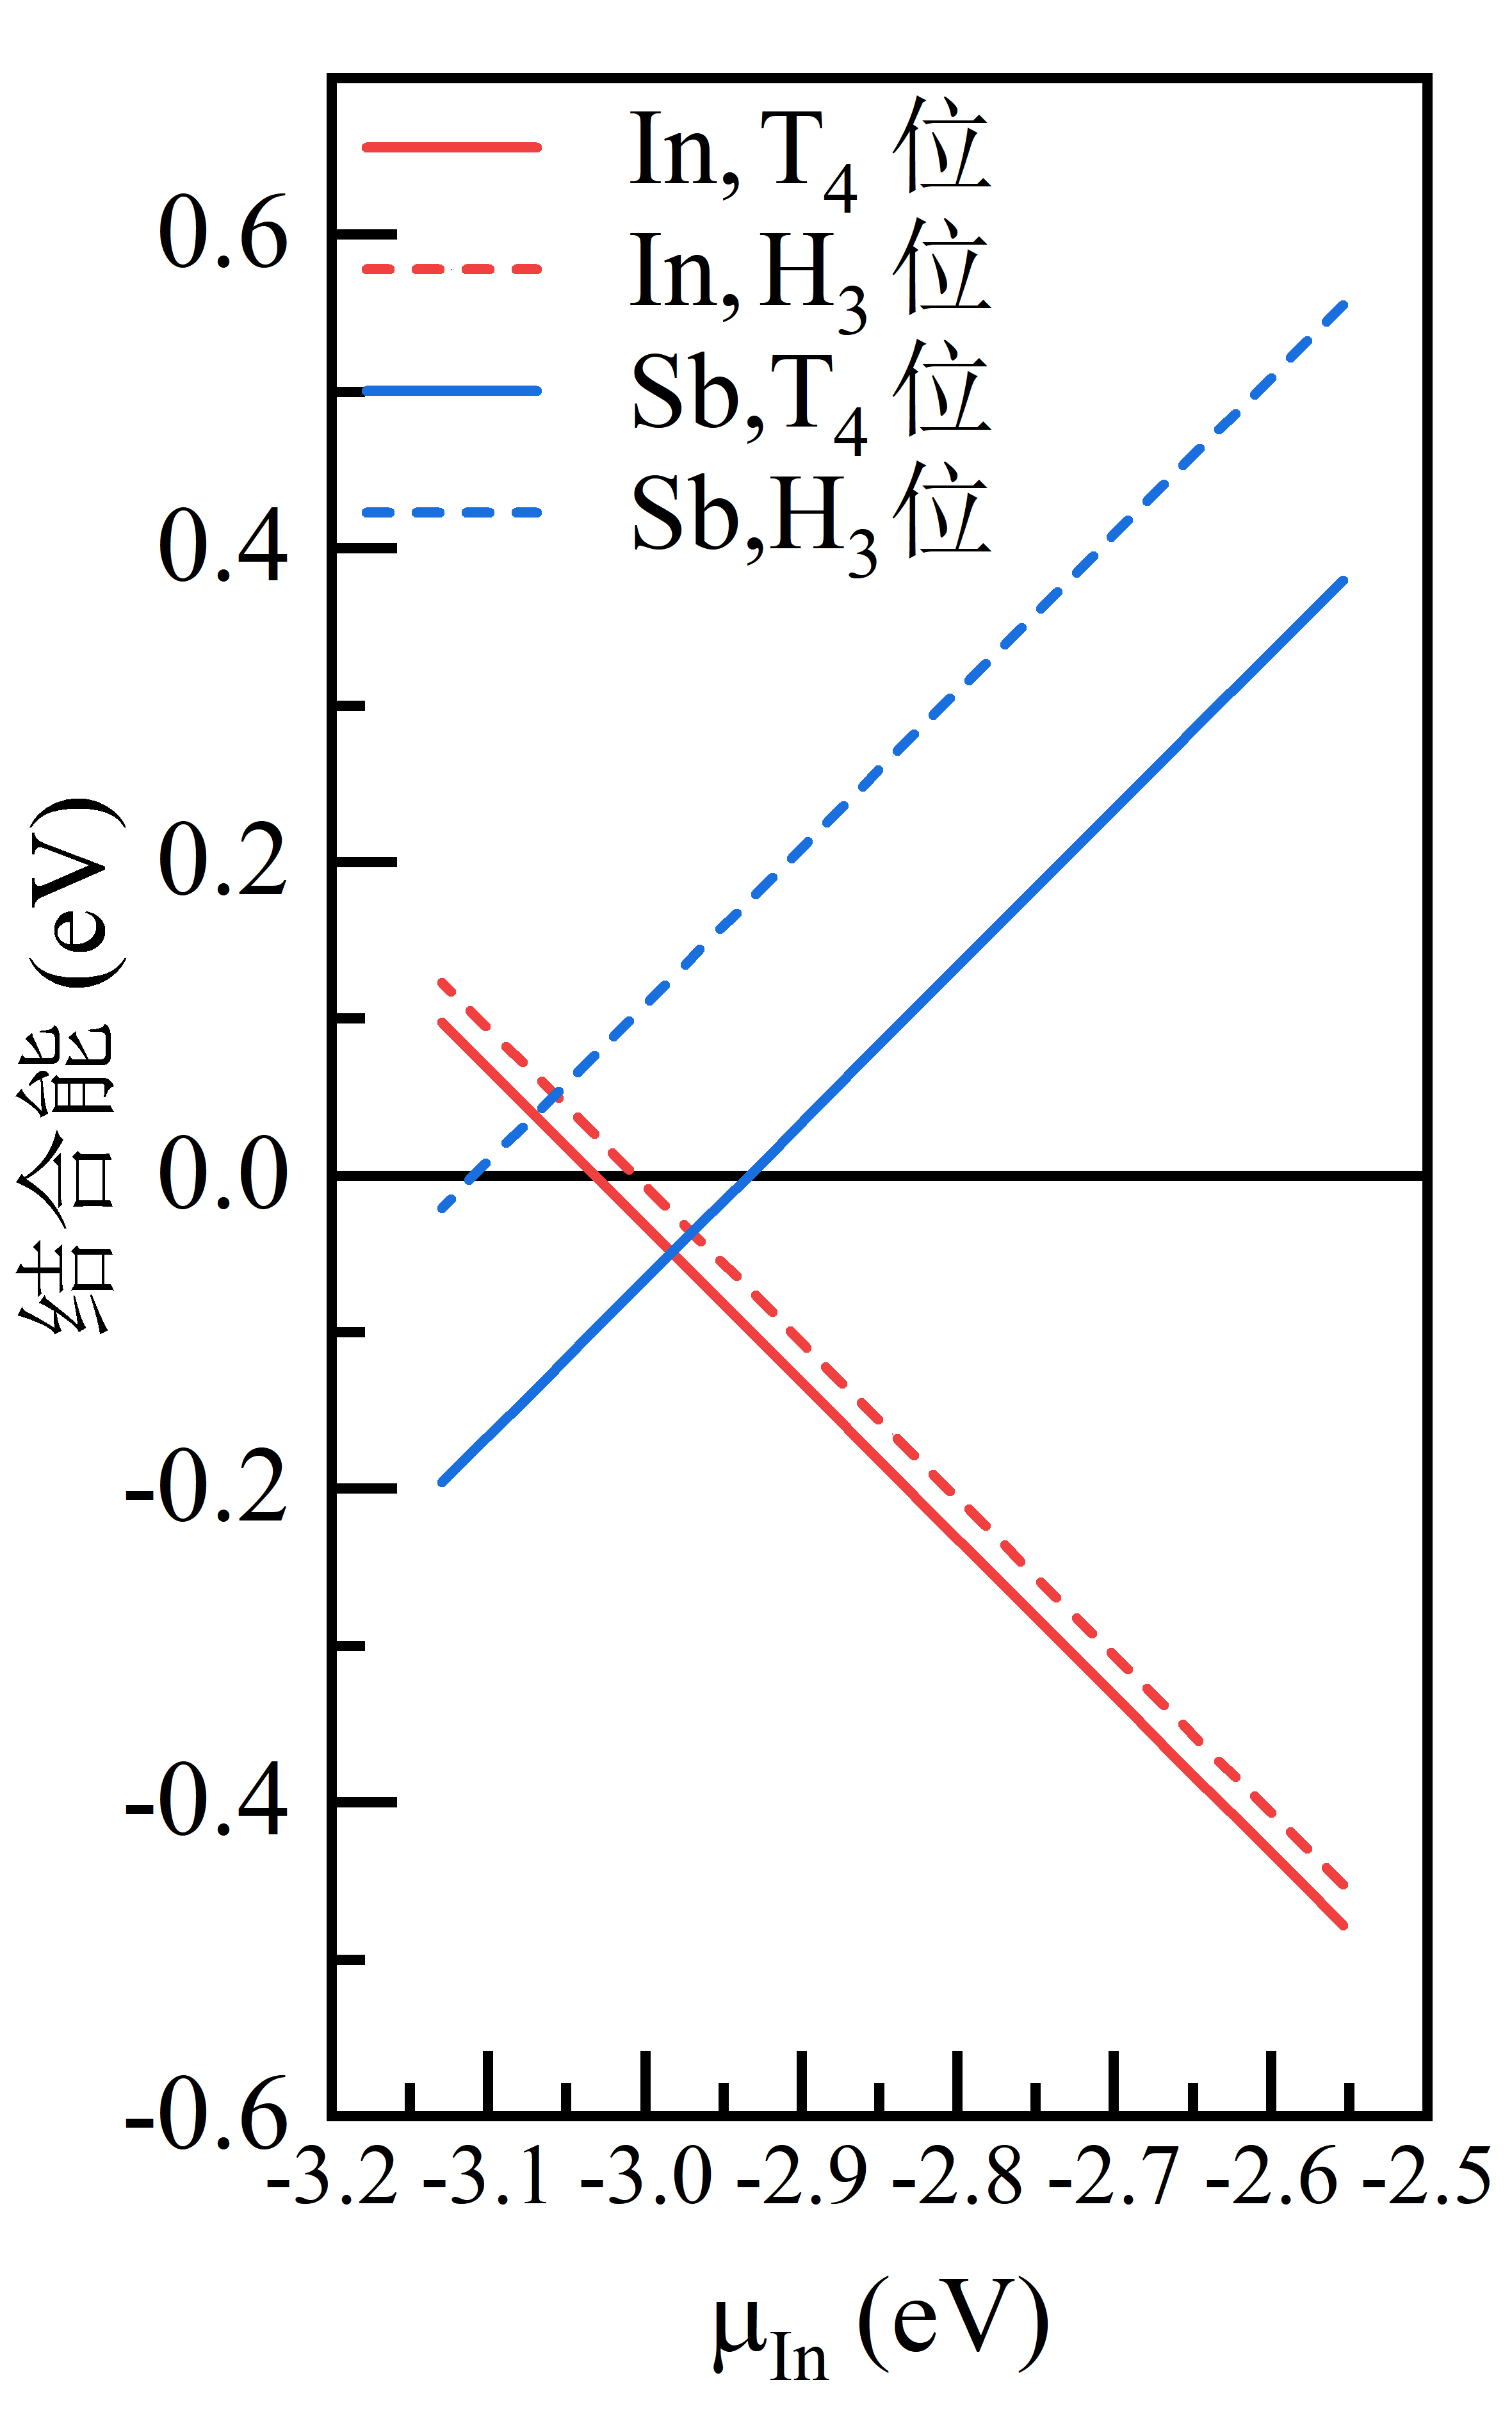
\includegraphics[]{pic/IS_DFT_adatomBind.png}
    }
    \subfloat[]{
        \label{fig:IS_structure_T4onBi}
        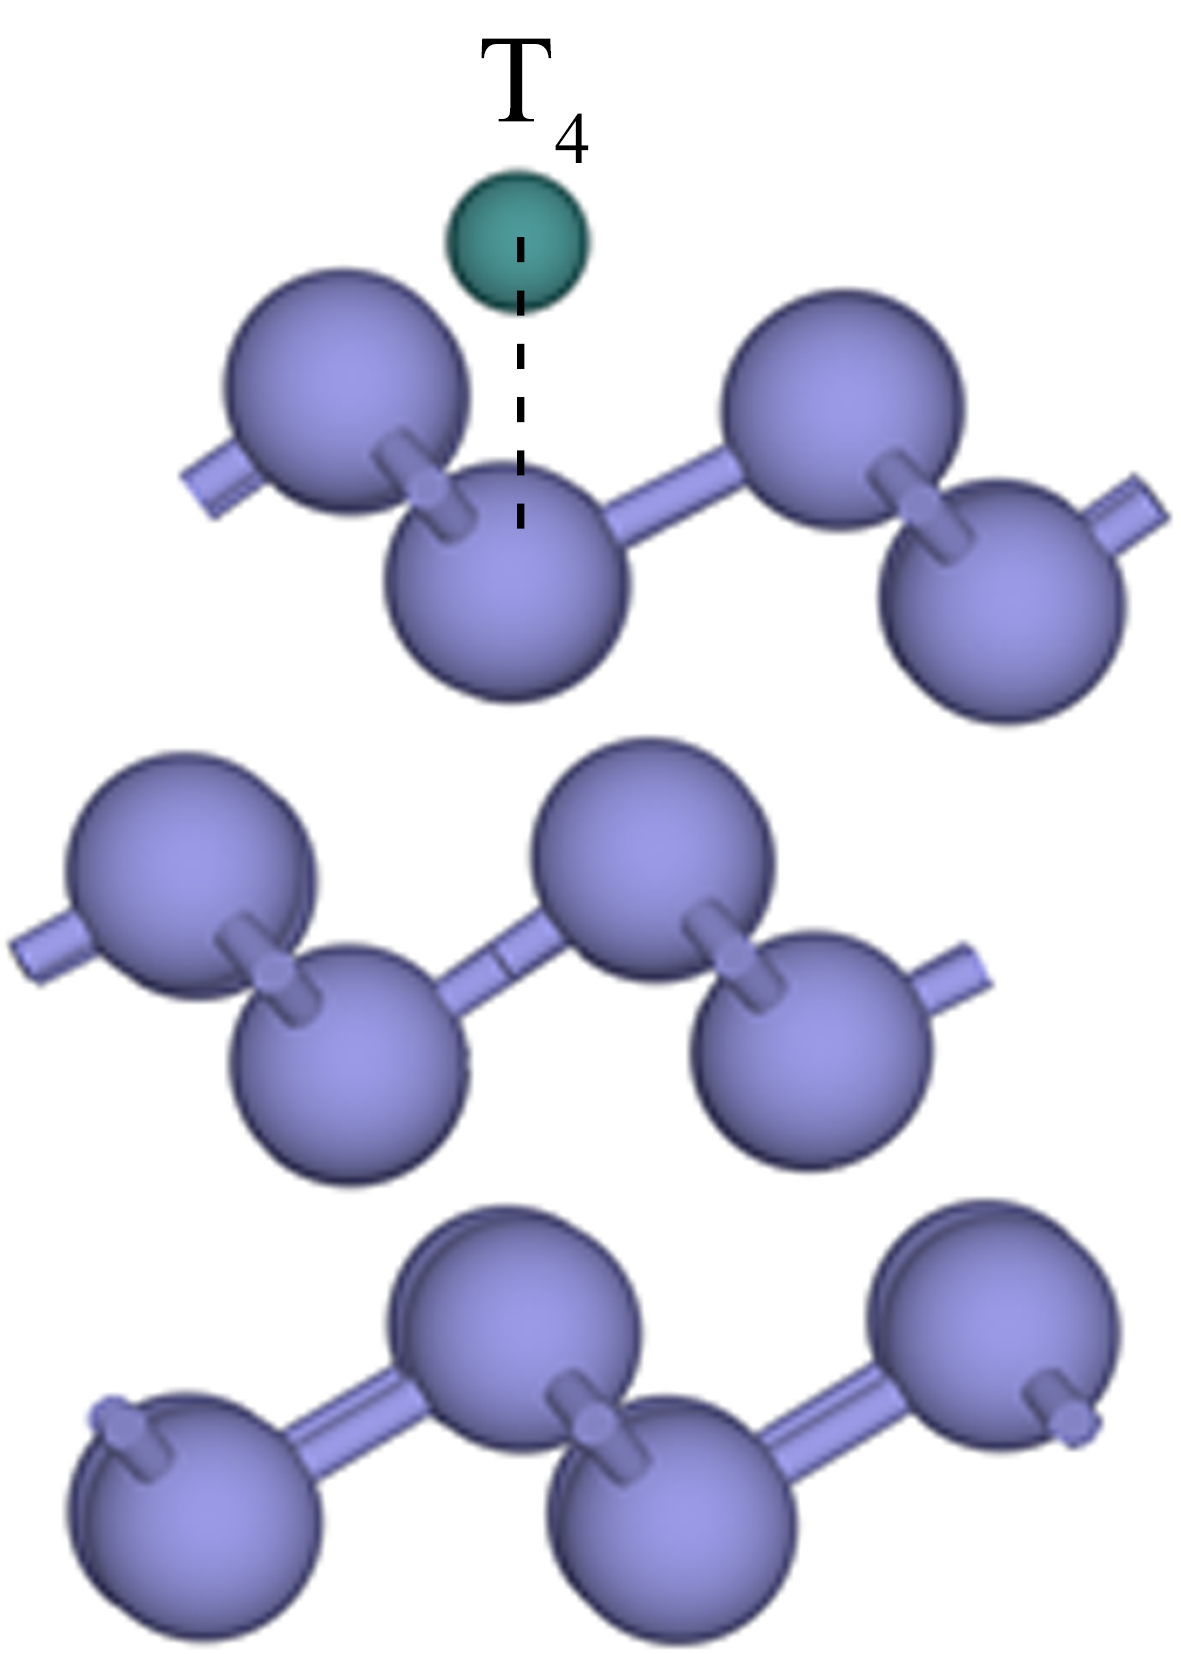
\includegraphics[trim={0, -20, 0 0},clip]{pic/IS_structure_T4onBi.png}
    }
    \subfloat[]{
        \label{fig:IS_structure_H3onBi}
        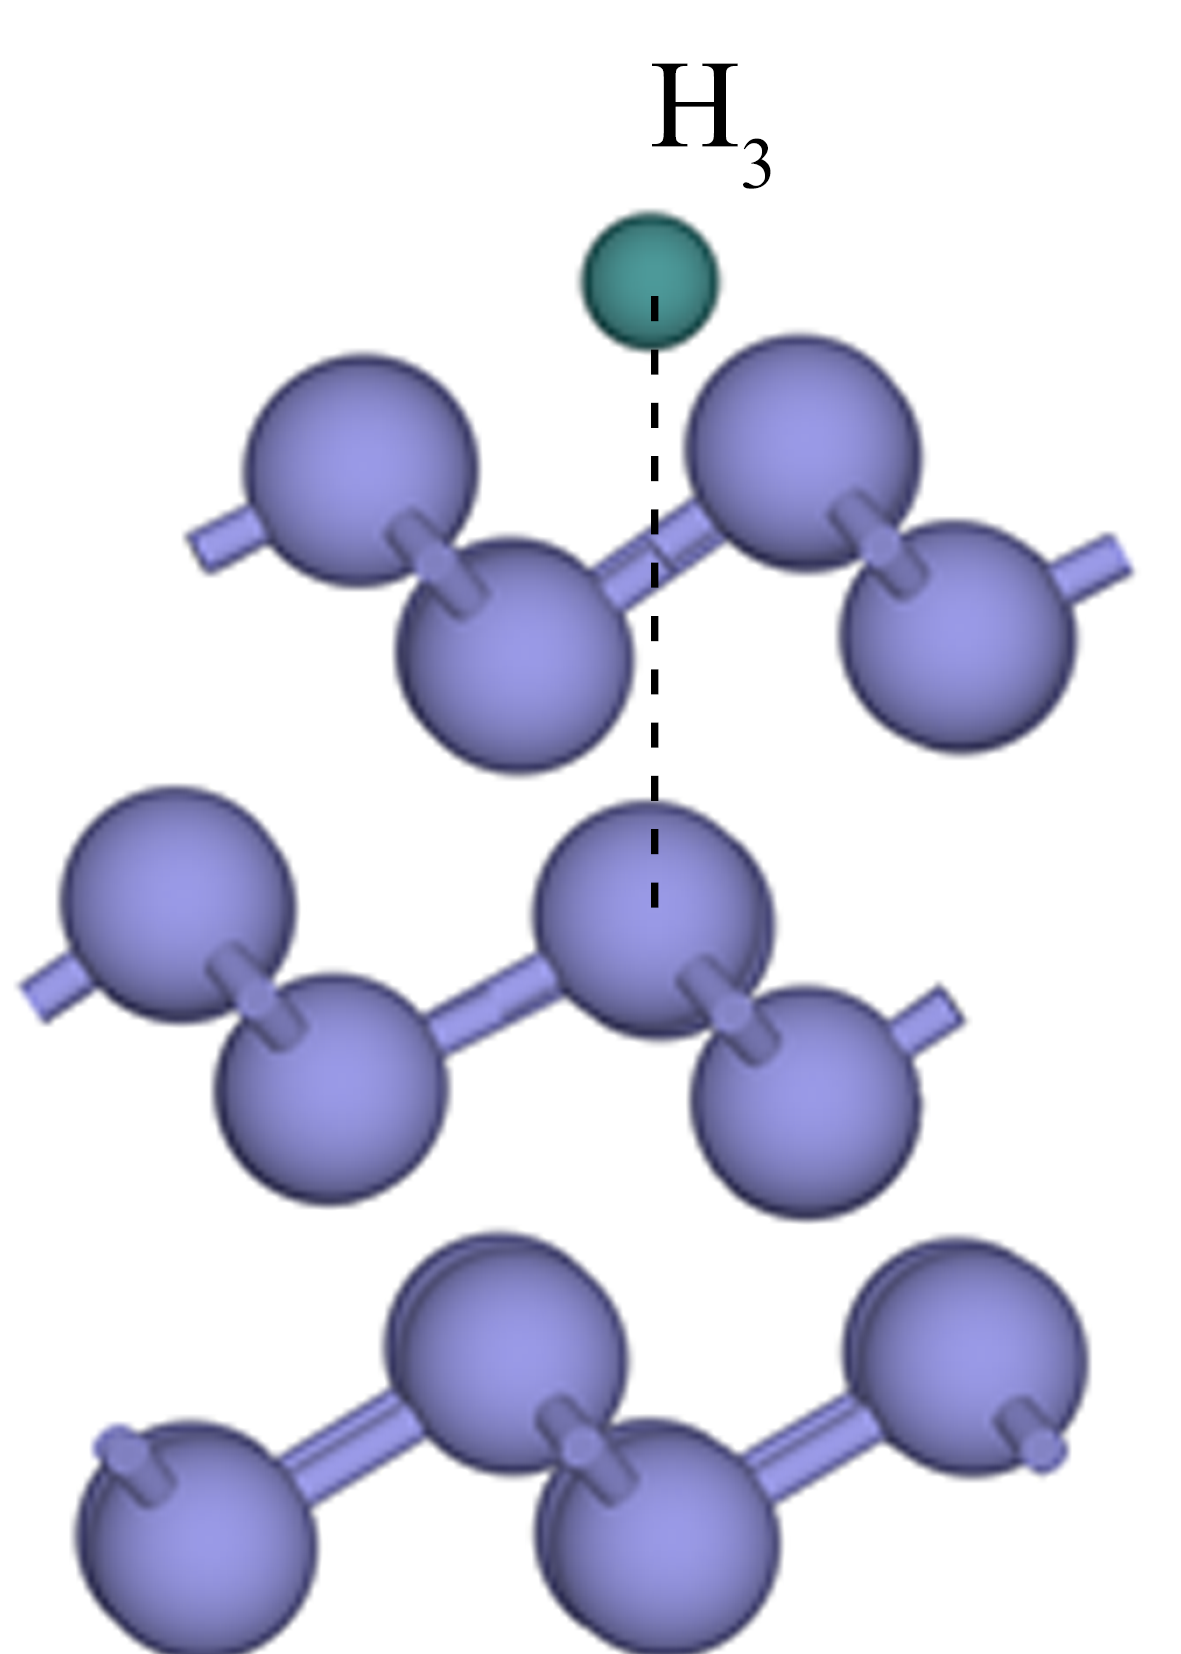
\includegraphics[trim={0, -20, 0 0},clip]{pic/IS_structure_H3onBi.png}
    }
    \caption{\cemb{Bi(001)}衬底表面\cemb{In}和\cemb{Sb}吸附原子的结合能和吸附位点。(a)吸附原子结合能。(b)吸附位点T4。(c)吸附位点H3。 原子结构图中,\cemb{Bi}原子使用蓝色表示,吸附原子(\cemb{In}、\cemb{Sb})用绿色表示。}
    \label{fig:IS_Bi_adatoms}
\end{figure}

对于$\muVar{adatom}{}$为吸附原子的化学势,由于生长环境下\cemb{InSb}块体的化学平衡,我们有\chinesecolon
\[
    \muVar{In}{}+\muVar{Sb}{}=\energyVar{InSb}{tot}=\energyVar{In\left(Bulk\right)}{}+\energyVar{Sb\left(Bulk\right)}{}+\delta H_{f}\left(\cemb{InSb}\right)
\]

其中$\energyVar{InSb}{tot}$、$\energyVar{In\left(Bulk\right)}{}$和$\energyVar{Sb\left(Bulk\right)}{}$为\cemb{InSb}块体,\cemb{In}块体和\cemb{Sb}块体的能量。因此,在生长气氛中\cemb{InSb}的化学平衡下,$\muVar{In}{}$的变化范围为$\muVar{In}{}\leqslant \energyVar{Sb\left(Bulk\right)}{}+\Delta H_{\rm f}\left(\cemb{InSb}\right) \leqslant \energyVar{In\left(Bulk\right)}{}$,代表\cemb{In}的化学势$\muVar{In}{}$由纯\cemb{Sb}的生长环境变化到纯\cemb{In}的生长环境。
 
对于吸附在$\TfourSite$位点的\cemb{In}原子,计算所得的在纯\cemb{In}环境下的结合能为\SI{-0.48}{\electronvolt},高于在纯\cemb{Sb}环境下同样吸附在$\TfourSite$位点的\cemb{Sb}原子的结合能(\SI{-0.19}{\electronvolt})。更高的结合能意味着相比于\cemb{Sb}原子,在能量最低的驱动下有更多的\cemb{In}原子从块体的状态分离并以吸附原子的状态沉积到\cemb{Bi(001)}的表面。

\begin{figure}[htb]
    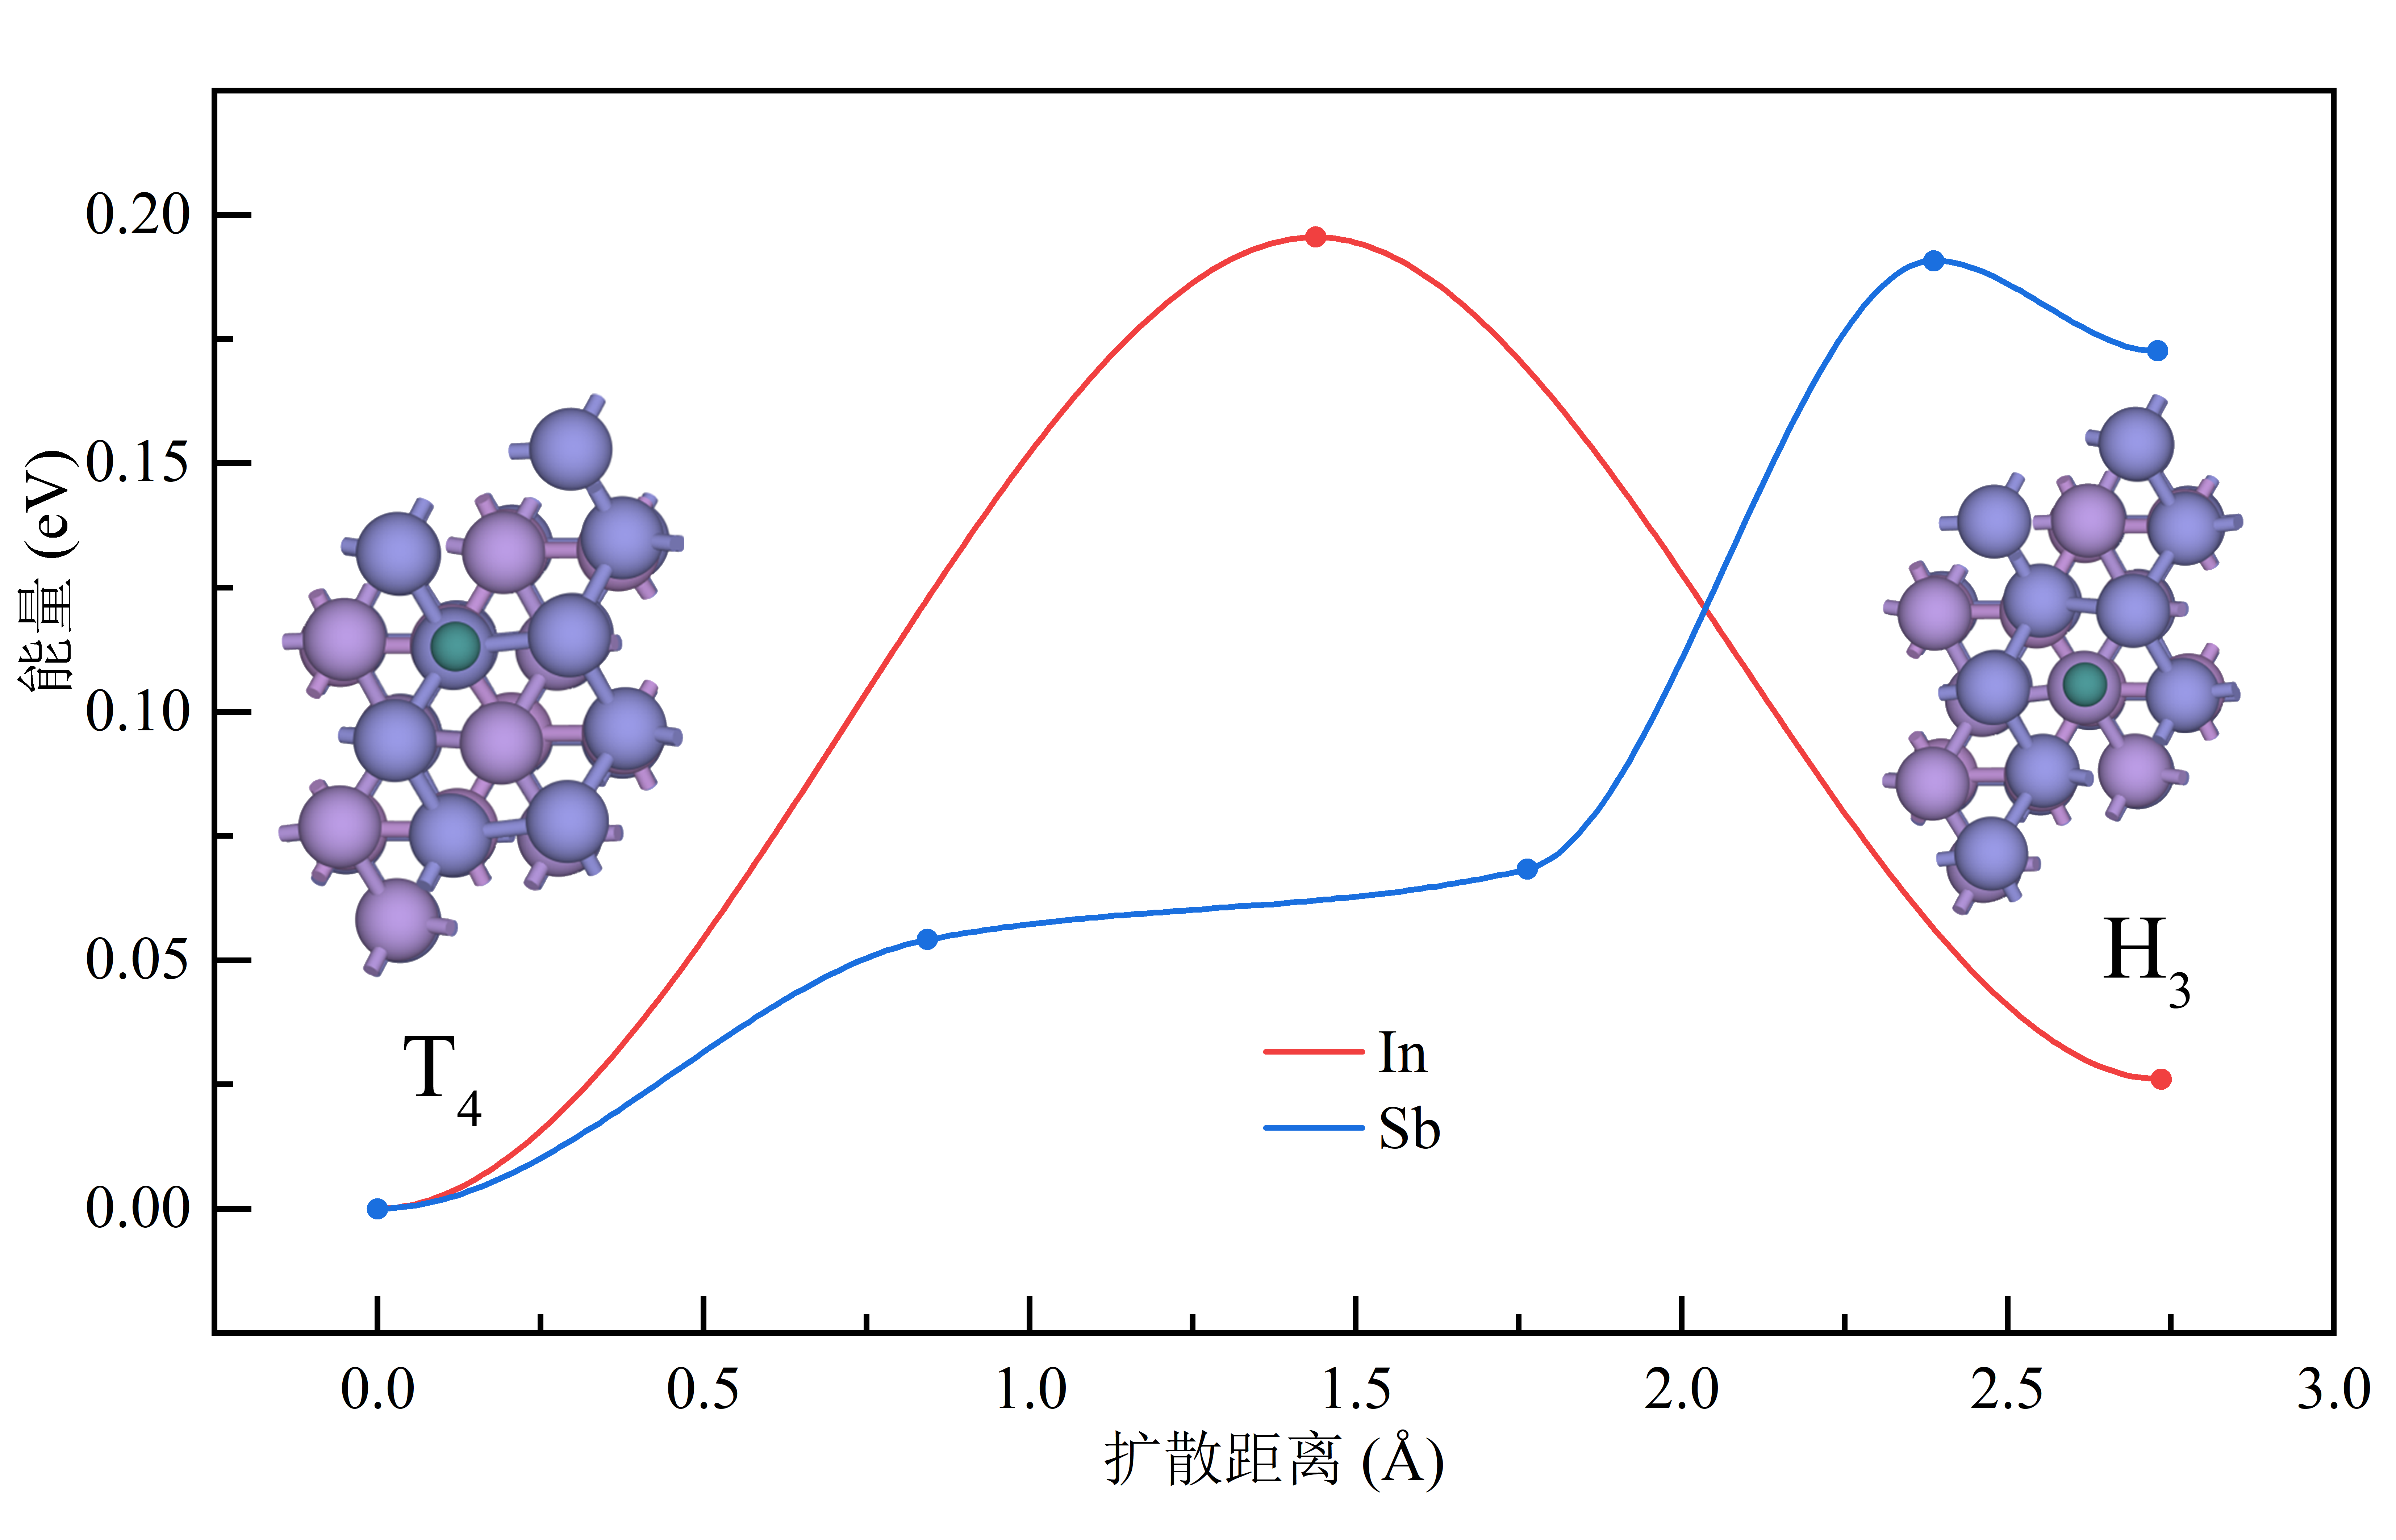
\includegraphics{pic/IS_DFT_adatomDiff.png}
    \caption{\cemb{Bi(001)}衬底表面\cemb{In}和\cemb{Sb}吸附原子的迁移势垒}
    \label{fig:IS_DFT_adatomDiff}
\end{figure}


\subsection{单层锑化铟的极性演化}
\begin{figure}[htb]
    \subfloat[]{
        \label{fig:IS_structure_1Linsb_04}
        \begin{tabular}{c}
            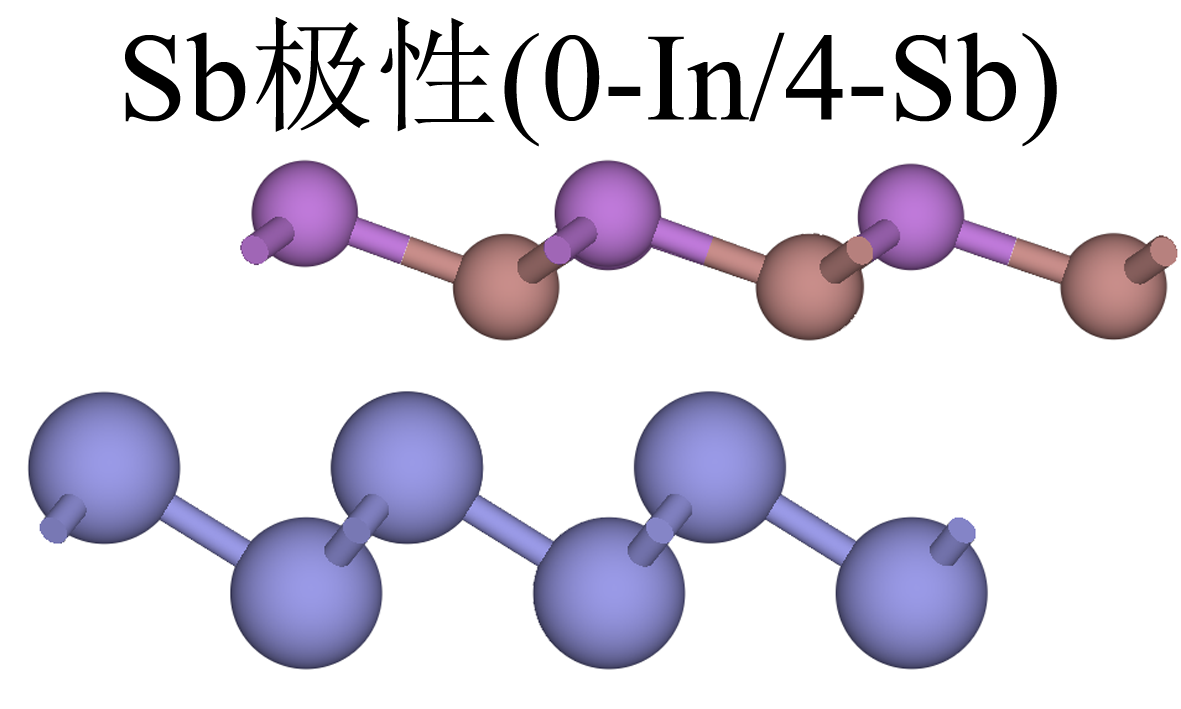
\includegraphics[width=0.28\textwidth]{pic/IS_structure_1Linsb_04side.png} \\
            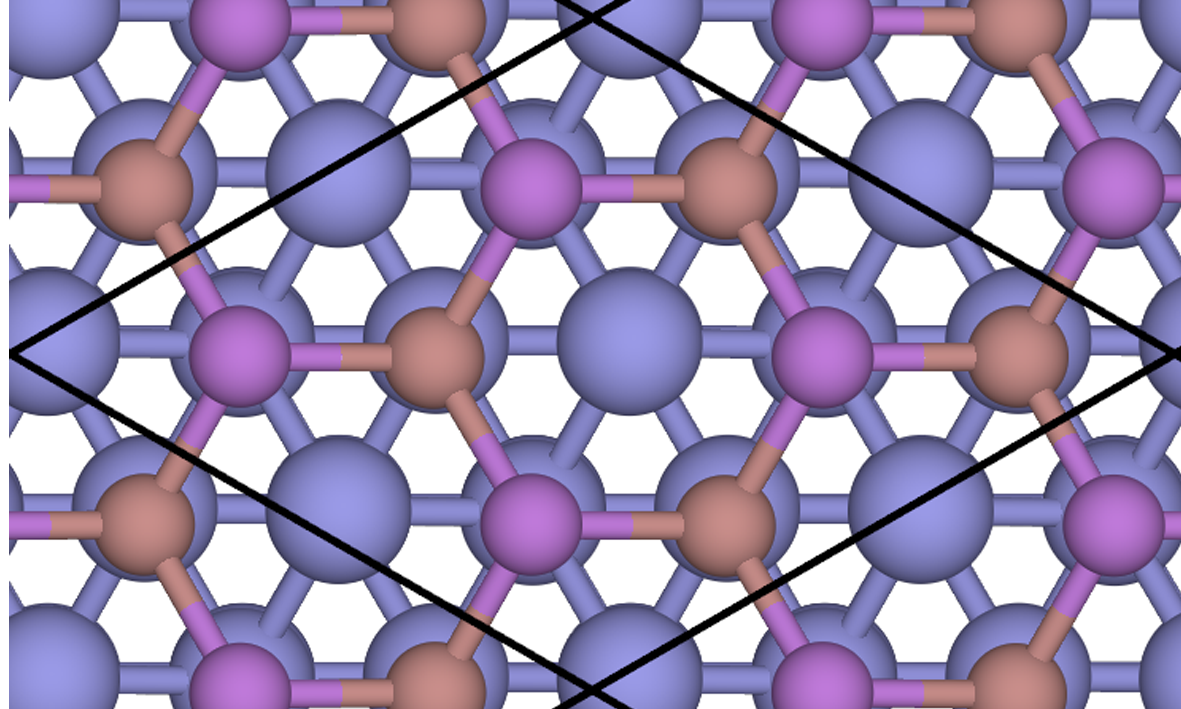
\includegraphics[width=0.28\textwidth]{pic/IS_structure_1Linsb_04top.png}
        \end{tabular}
    }
    \subfloat[]{
        \label{fig:IS_structure_1Linsb_13}
        \begin{tabular}{c}
            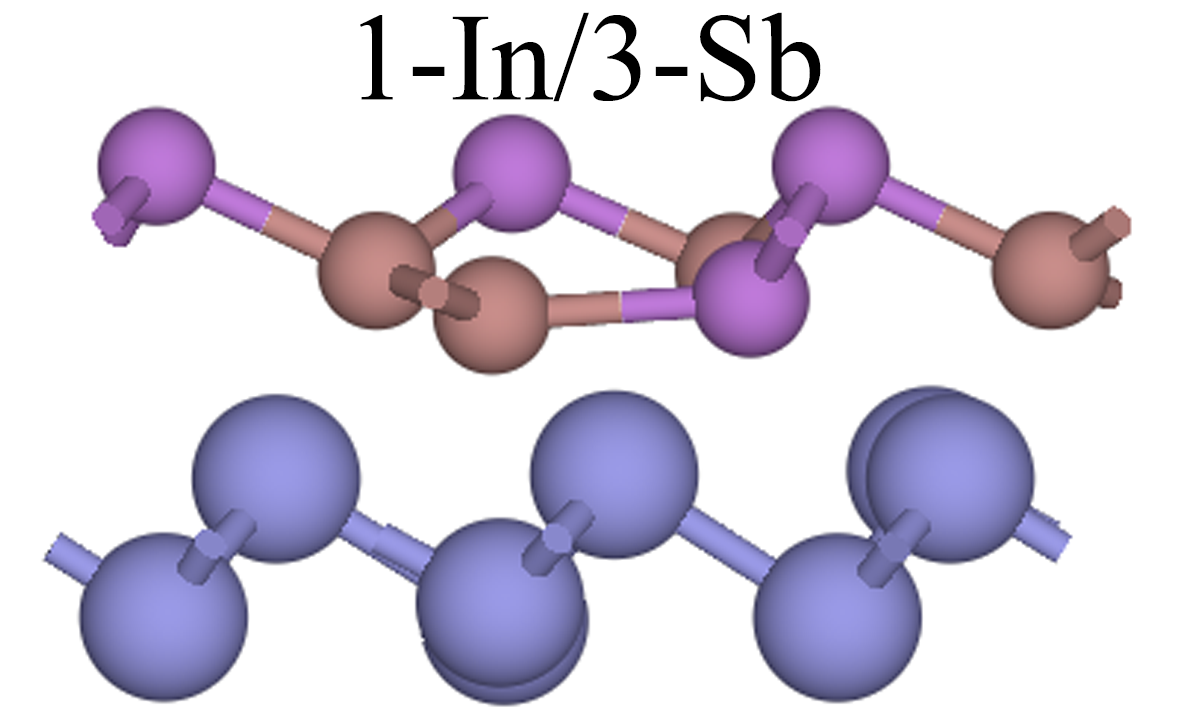
\includegraphics[width=0.28\textwidth]{pic/IS_structure_1Linsb_13side.png} \\
            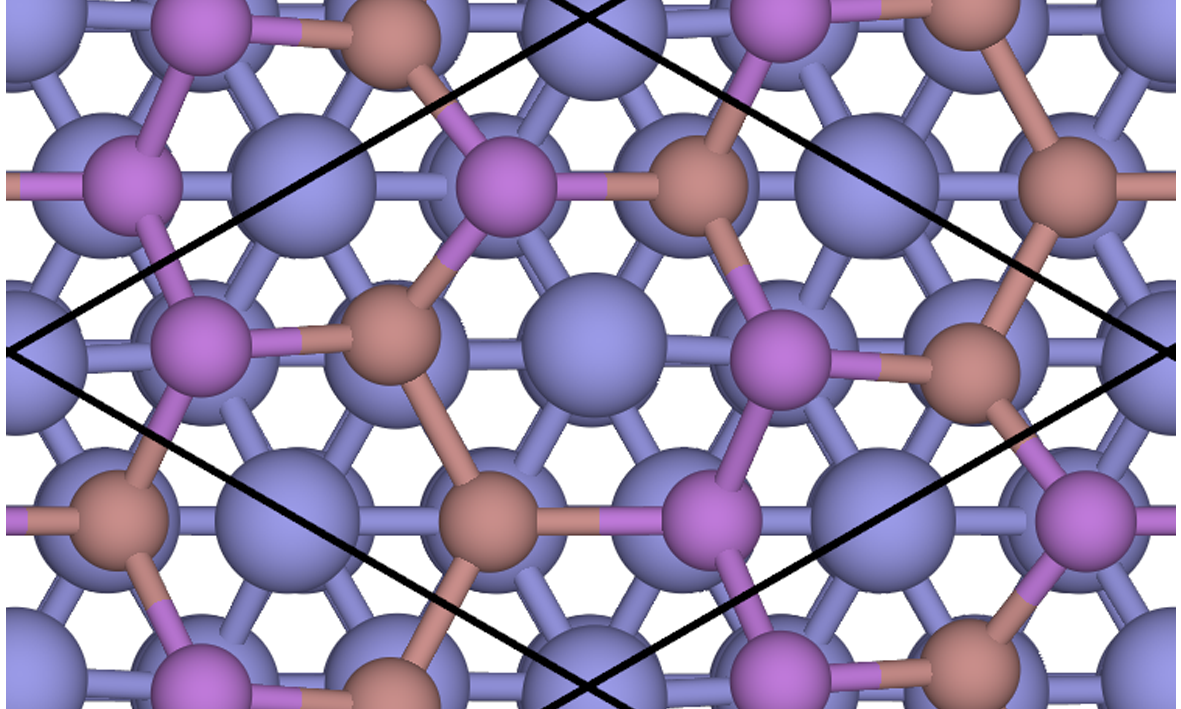
\includegraphics[width=0.28\textwidth]{pic/IS_structure_1Linsb_13top.png}
        \end{tabular}
    }
    \subfloat[]{
        \label{fig:IS_structure_1Linsb_22rec}
        \begin{tabular}{c}
            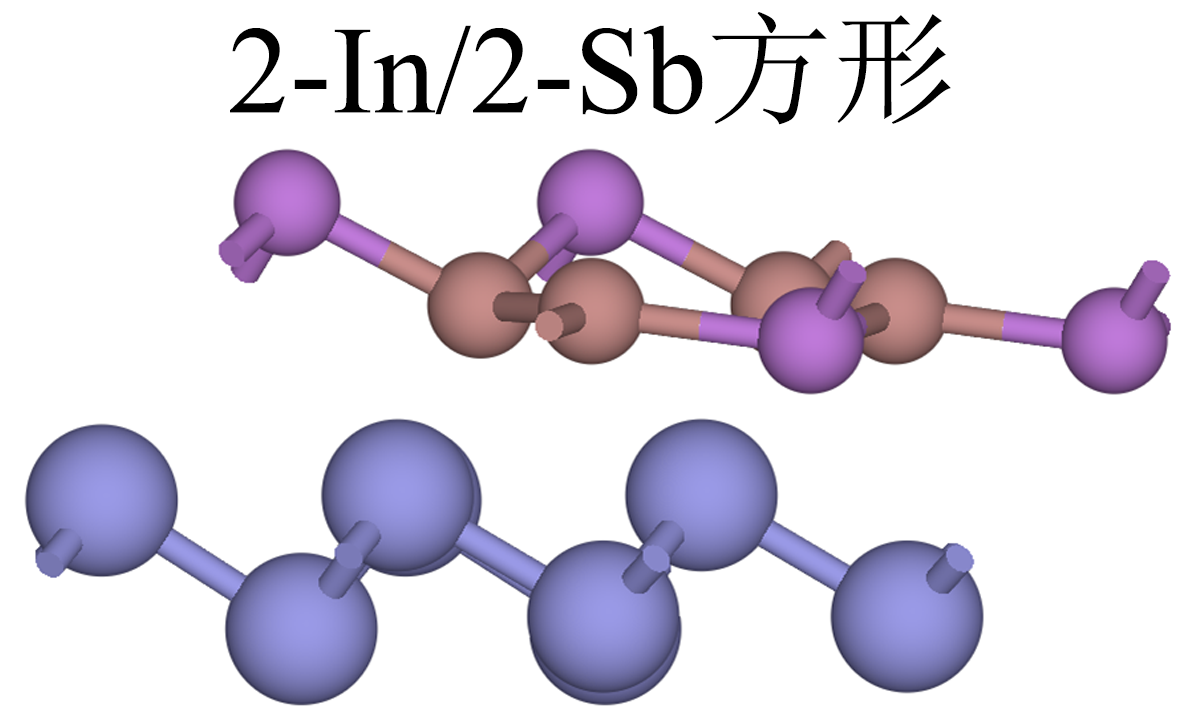
\includegraphics[width=0.28\textwidth]{pic/IS_structure_1Linsb_22recside.png} \\
            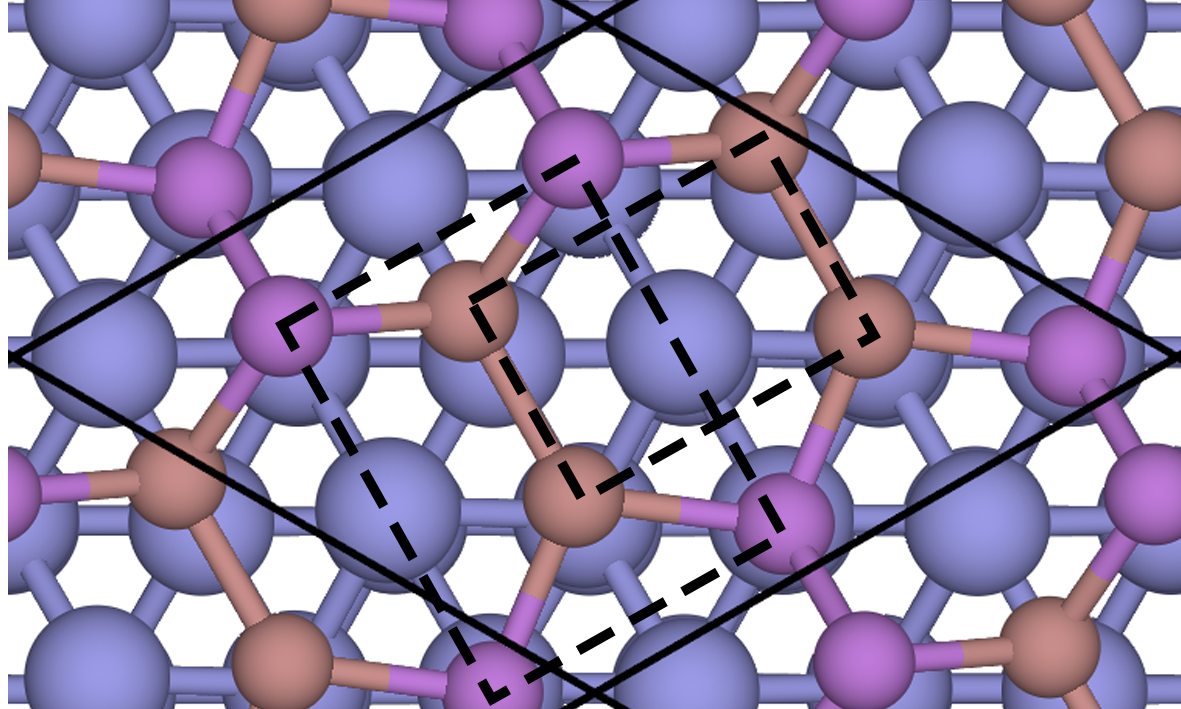
\includegraphics[width=0.28\textwidth]{pic/IS_structure_1Linsb_22rectop.png}
        \end{tabular}
    }\\[-1ex]
    \subfloat[]{
        \label{fig:IS_structure_1Linsb_22str}
        \begin{tabular}{c}
            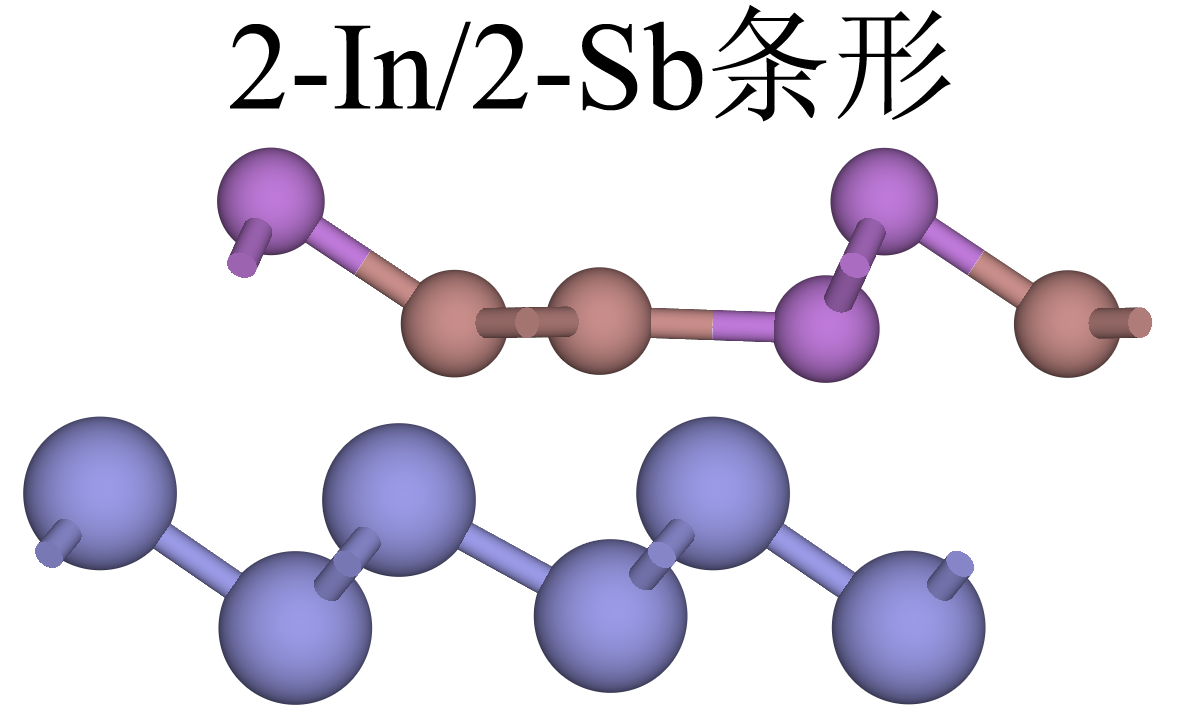
\includegraphics[width=0.28\textwidth]{pic/IS_structure_1Linsb_22strside.png} \\
            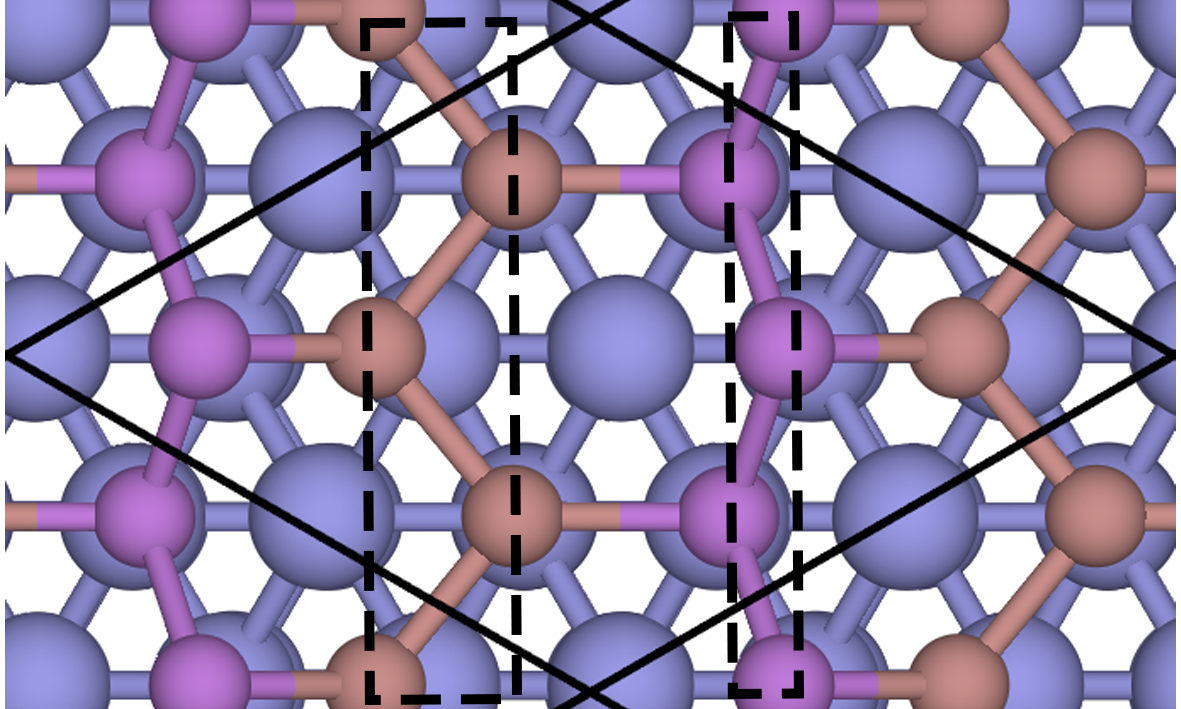
\includegraphics[width=0.28\textwidth]{pic/IS_structure_1Linsb_22strtop.png}
        \end{tabular}
    }
    \subfloat[]{
        \label{fig:IS_structure_1Linsb_31}
        \begin{tabular}{c}
            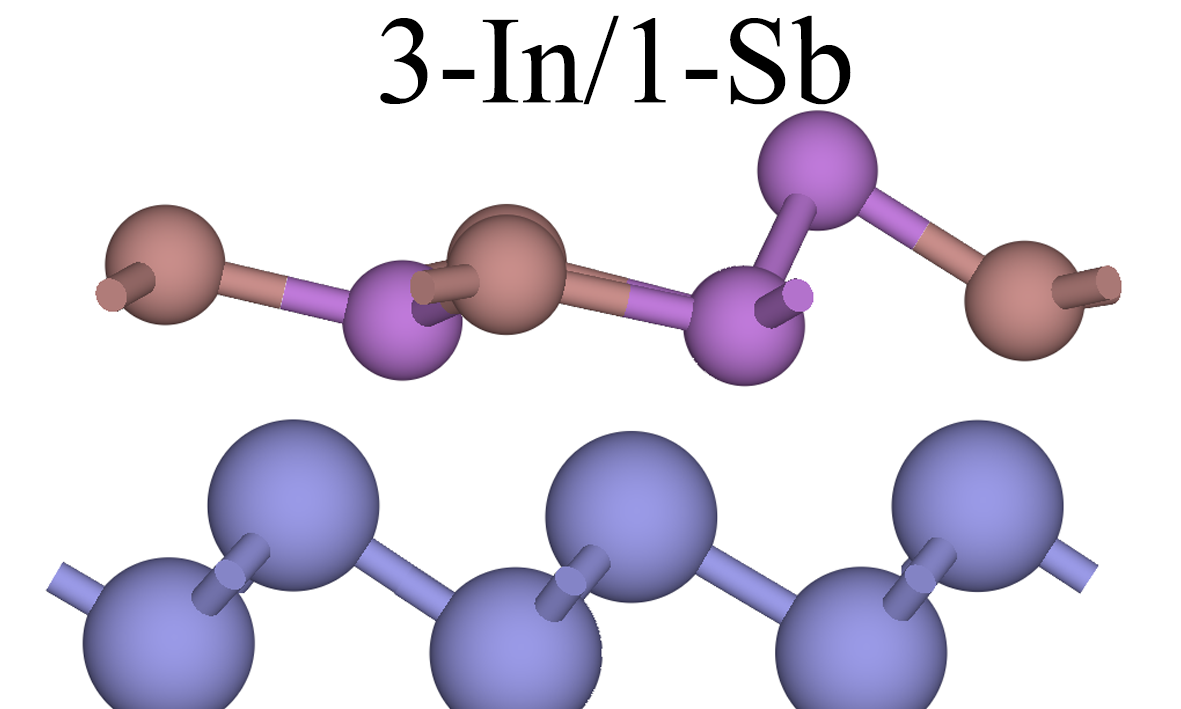
\includegraphics[width=0.28\textwidth]{pic/IS_structure_1Linsb_31side.png} \\
            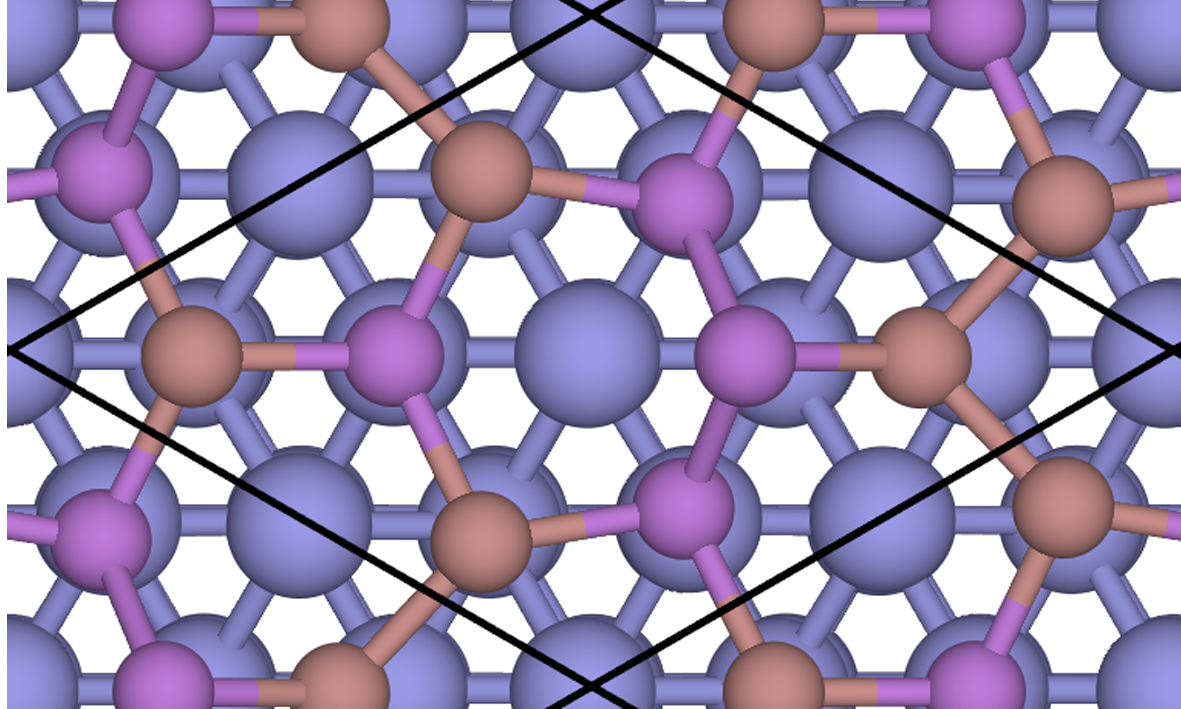
\includegraphics[width=0.28\textwidth]{pic/IS_structure_1Linsb_31top.png}
        \end{tabular}
    }
    \subfloat[]{
        \label{fig:IS_structure_1Linsb_40}
        \begin{tabular}{c}
            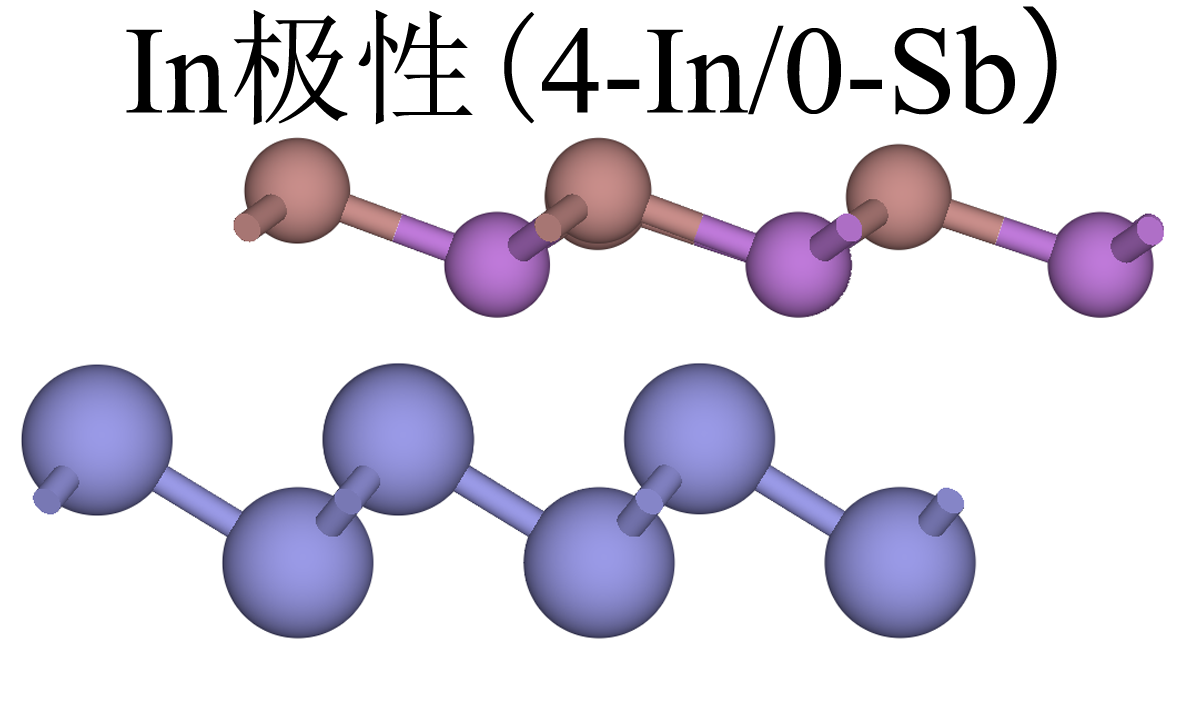
\includegraphics[width=0.28\textwidth]{pic/IS_structure_1Linsb_40side.png} \\
            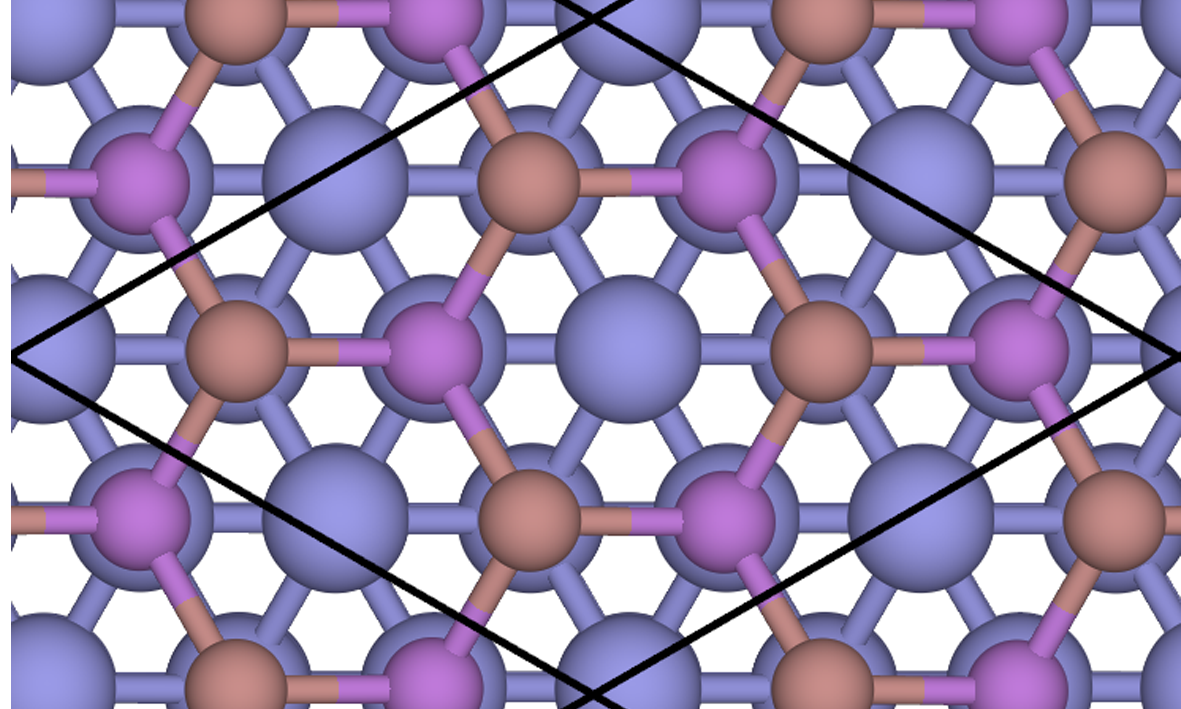
\includegraphics[width=0.28\textwidth]{pic/IS_structure_1Linsb_40top.png}
        \end{tabular}
    }
    \caption{\cemb{Bi(001)}衬底上不同极性单层\cemb{InSb}的原子结构。}
    \label{fig:IS_structure_1Linsb_allPolarity}
\end{figure}

\begin{figure}[htb]
    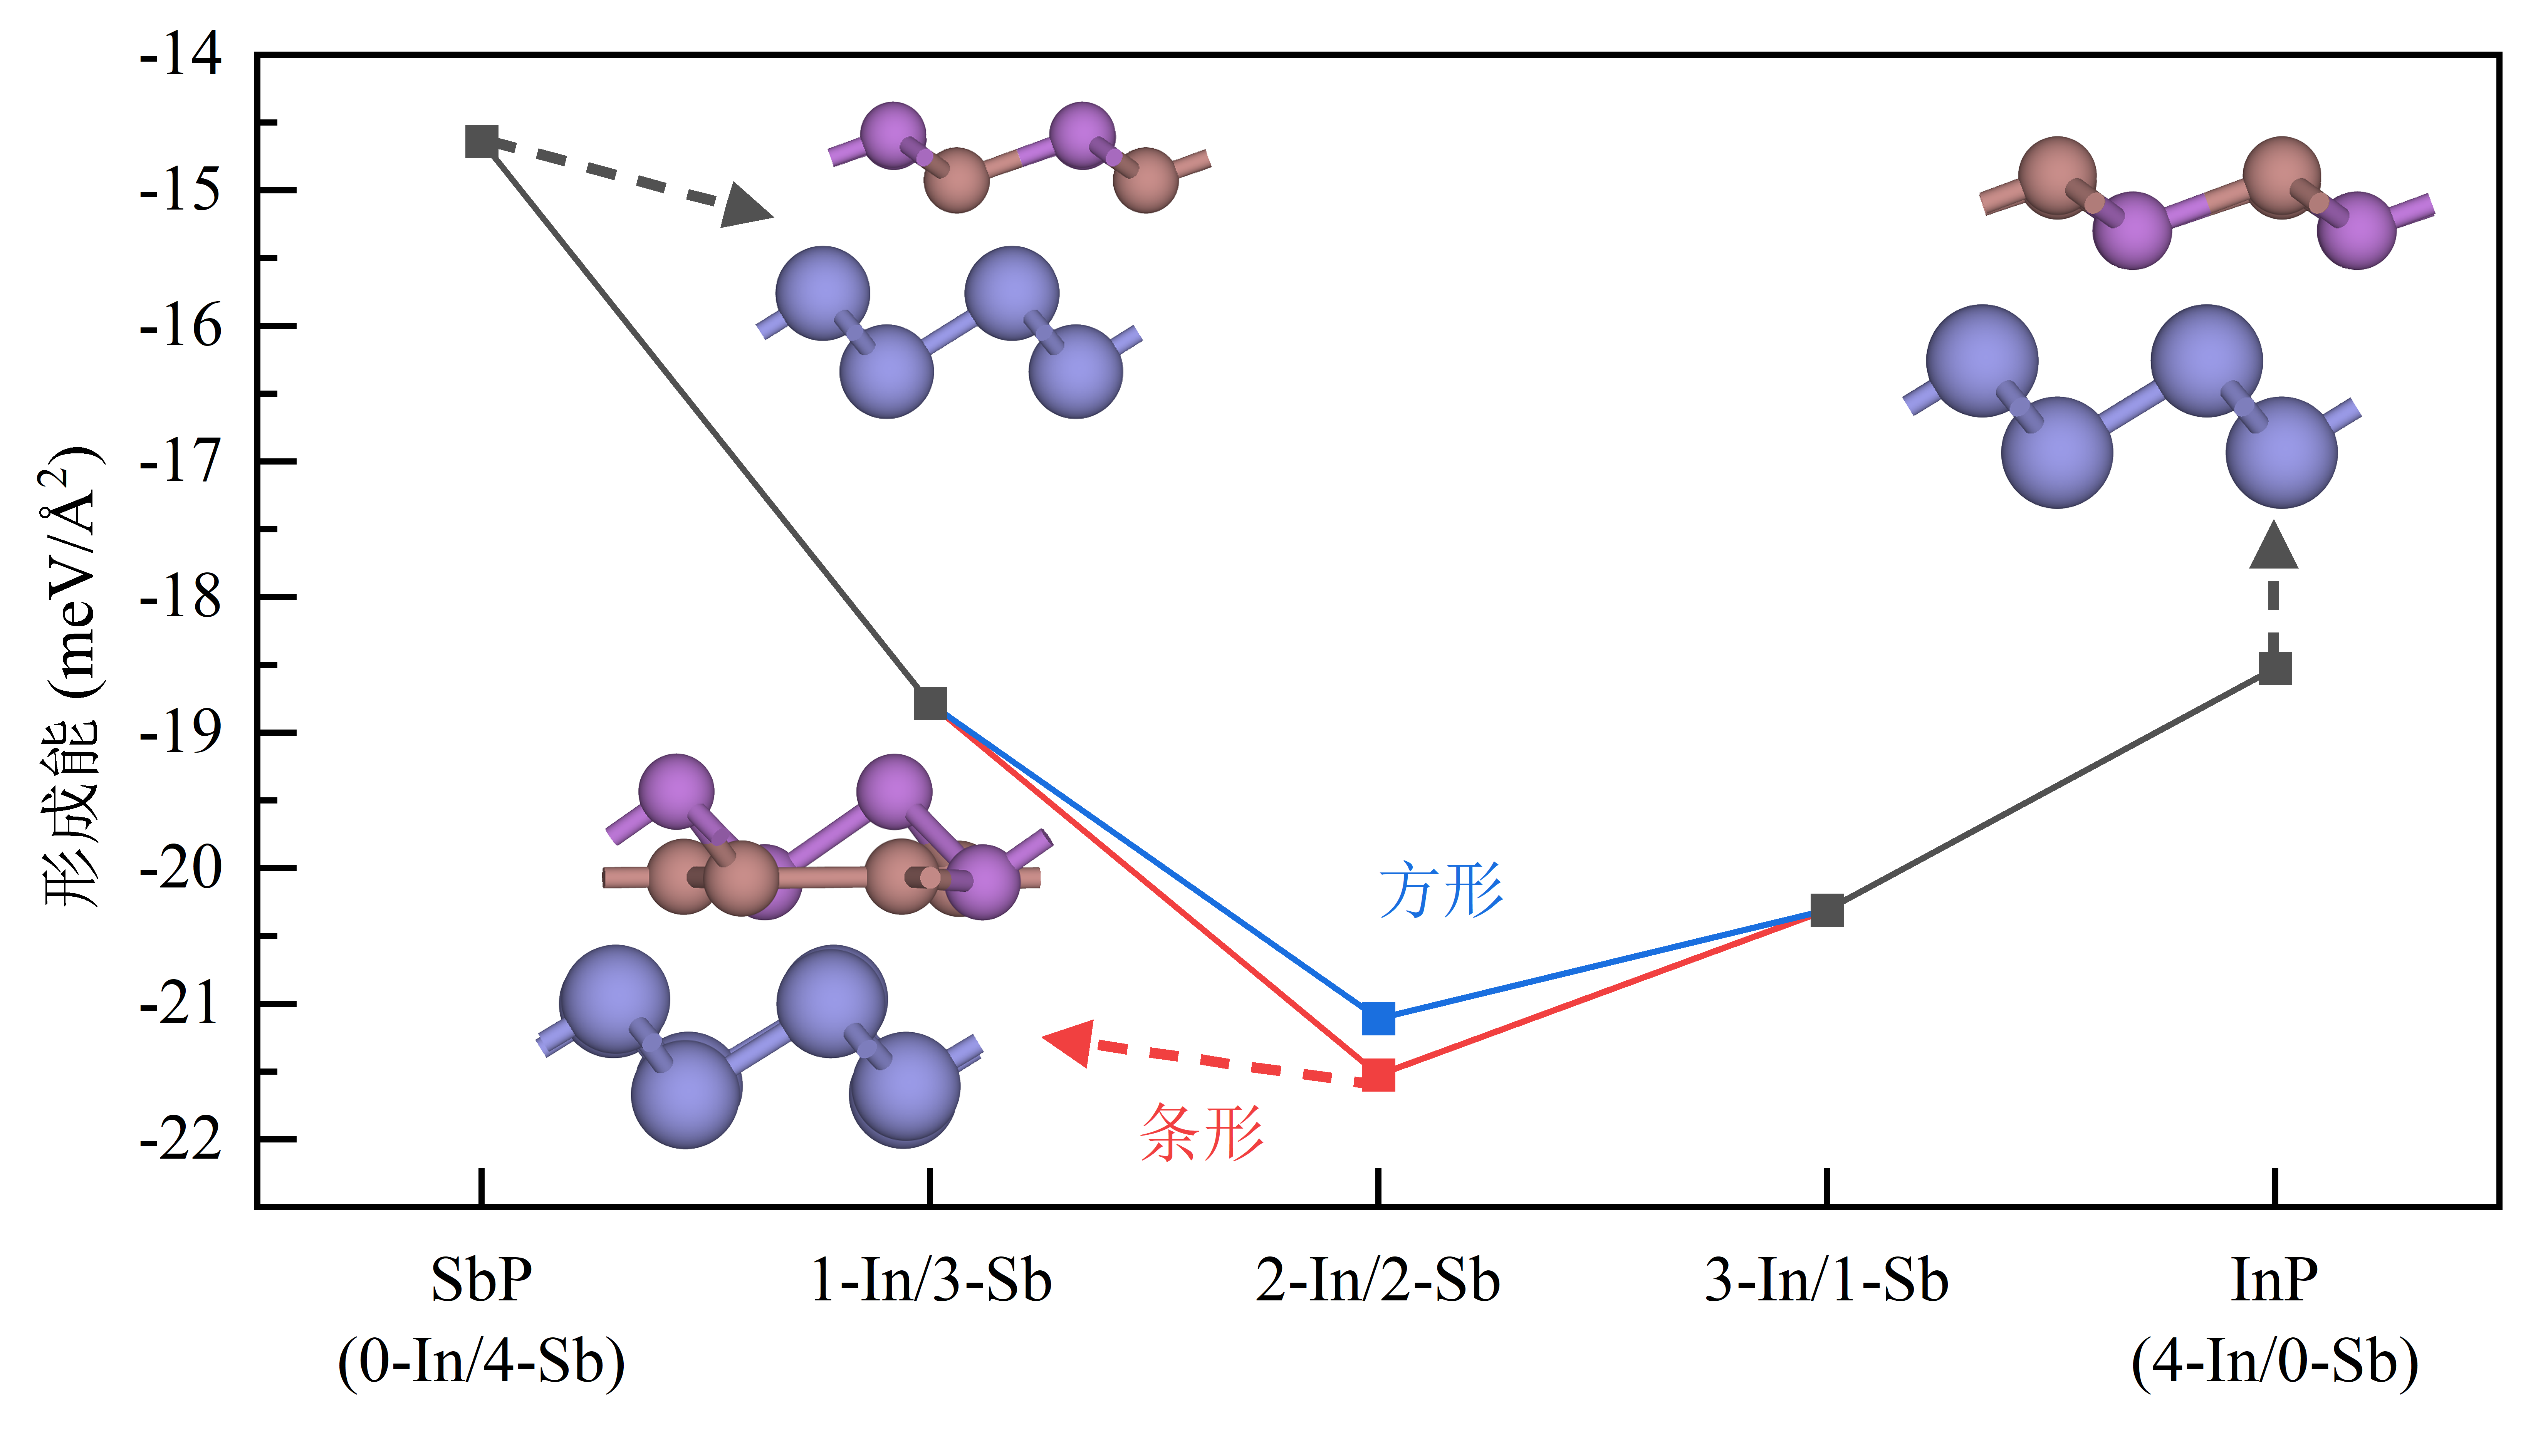
\includegraphics{pic/IS_DFT_1LInSb_all.png}
    \caption{\cemb{Bi(001)}衬底上不同极性单层\cemb{InSb}的形成能。}
    \label{fig:IS_DFT_1LInSb_all}
\end{figure}

\begin{figure}[htb]
    \subfloat[]{
        \label{fig:IS_structure_1Linsb_md0ps}
        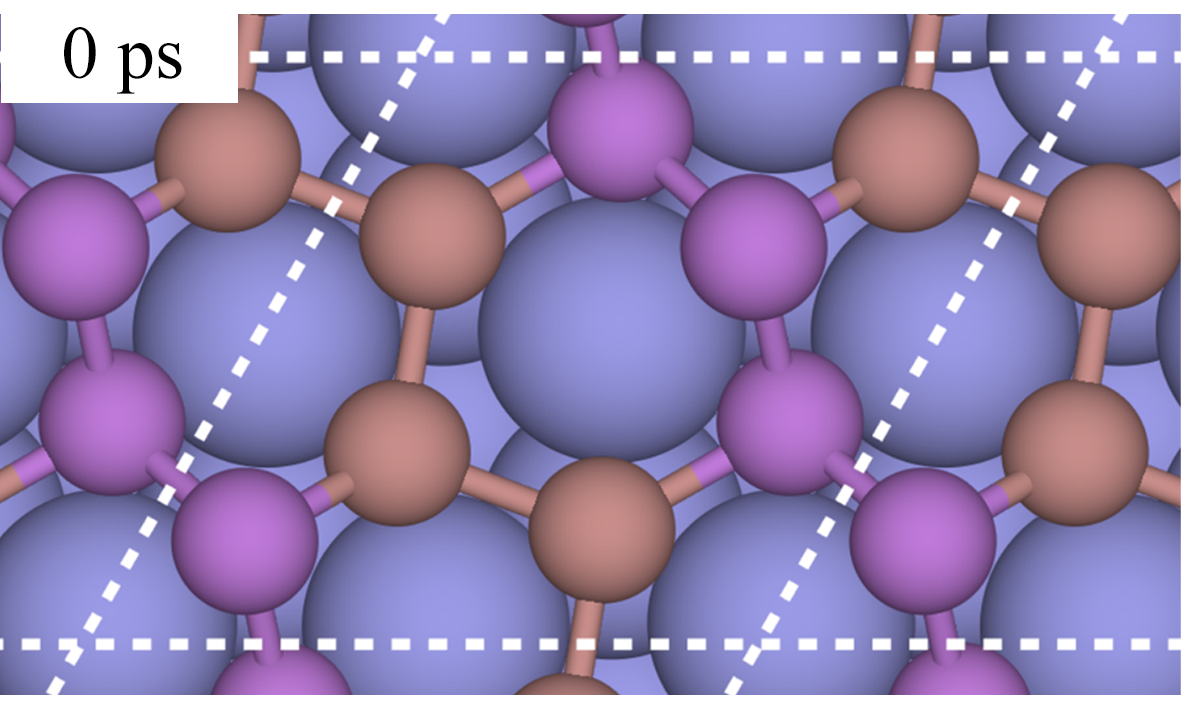
\includegraphics{pic/IS_structure_1Linsb_md0ps.png}
    }
    \subfloat[]{
        \label{fig:IS_structure_1Linsb_md10ps}
        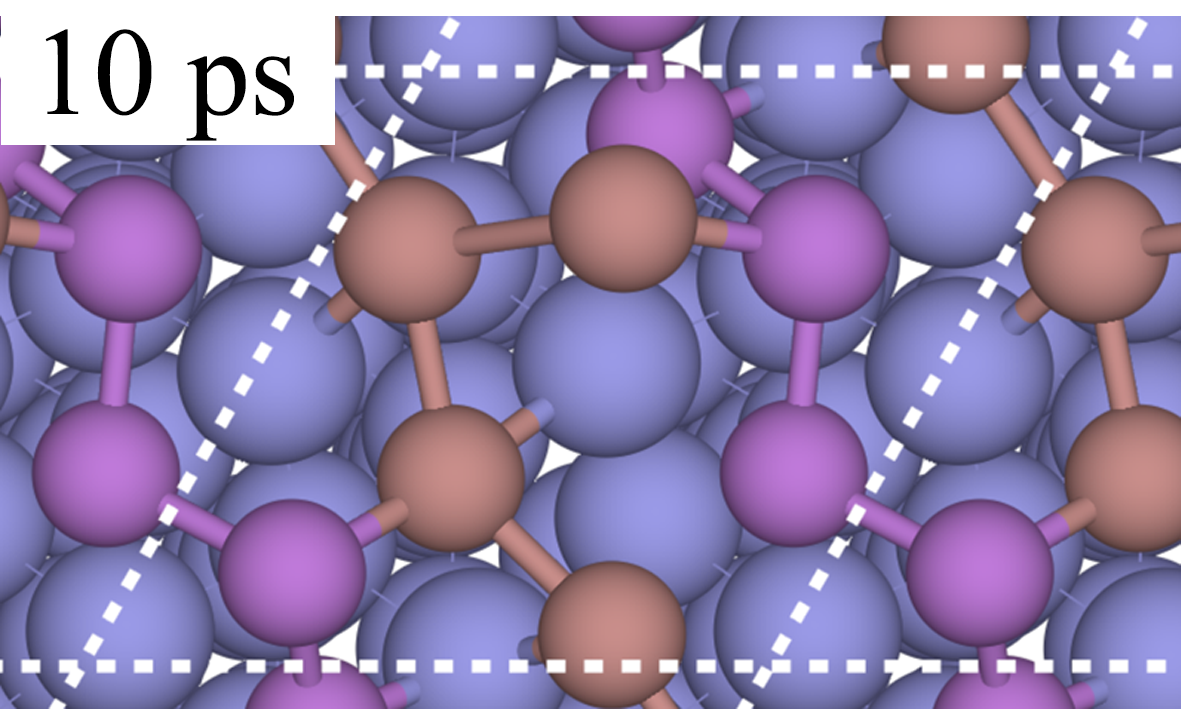
\includegraphics{pic/IS_structure_1Linsb_md10ps.png}
    }\\[-1ex]

    \subfloat[]{
        \label{fig:IS_structure_1Linsb_md20ps}
        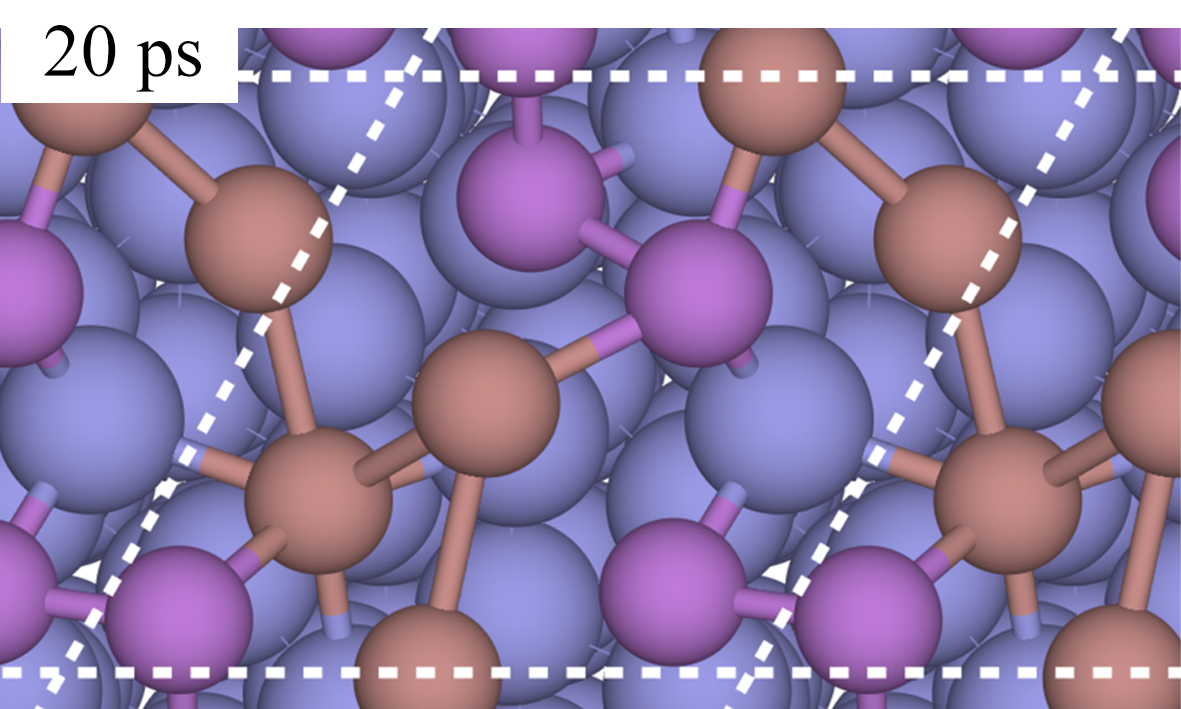
\includegraphics{pic/IS_structure_1Linsb_md20ps.png}
    }
    \subfloat[]{
        \label{fig:IS_structure_1Linsb_md30ps}
        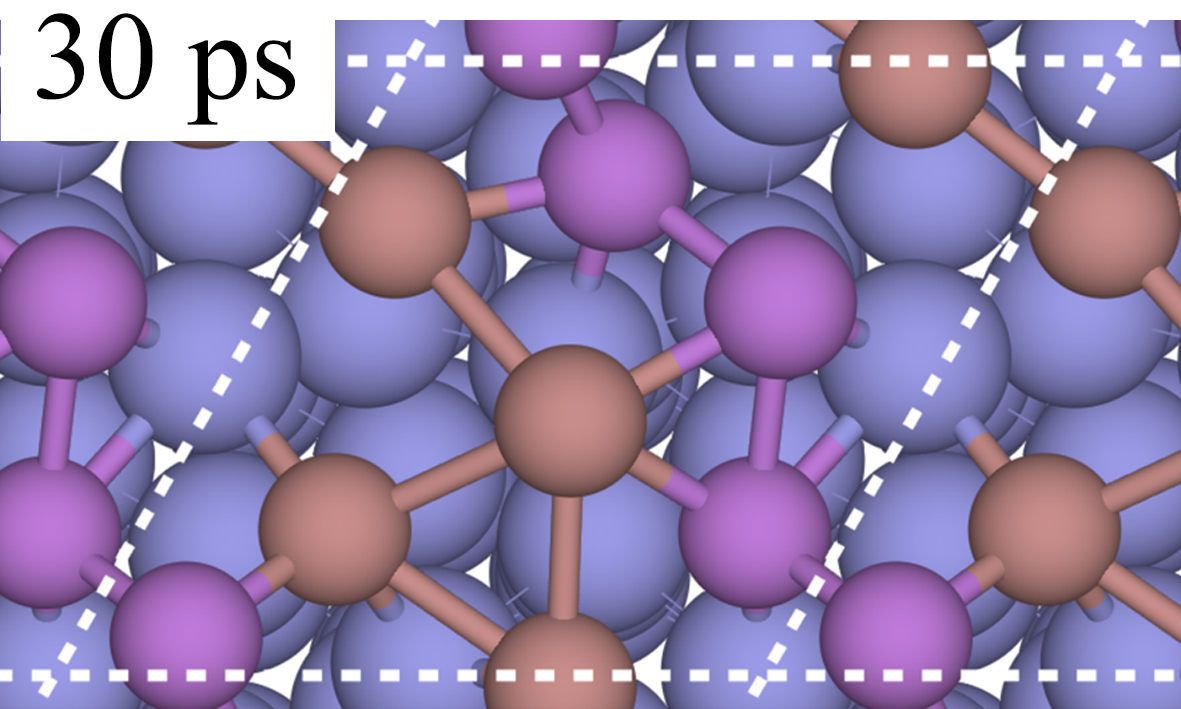
\includegraphics{pic/IS_structure_1Linsb_md30ps.png}
    }
    \caption{\cemb{Bi(001)}衬底上2-In/2-Sb条形极性\cemb{InSb}的分子动力学模拟结果。}
    \label{fig:IS_structure_1Linsb_md}
\end{figure}

\begin{figure}[htb]
    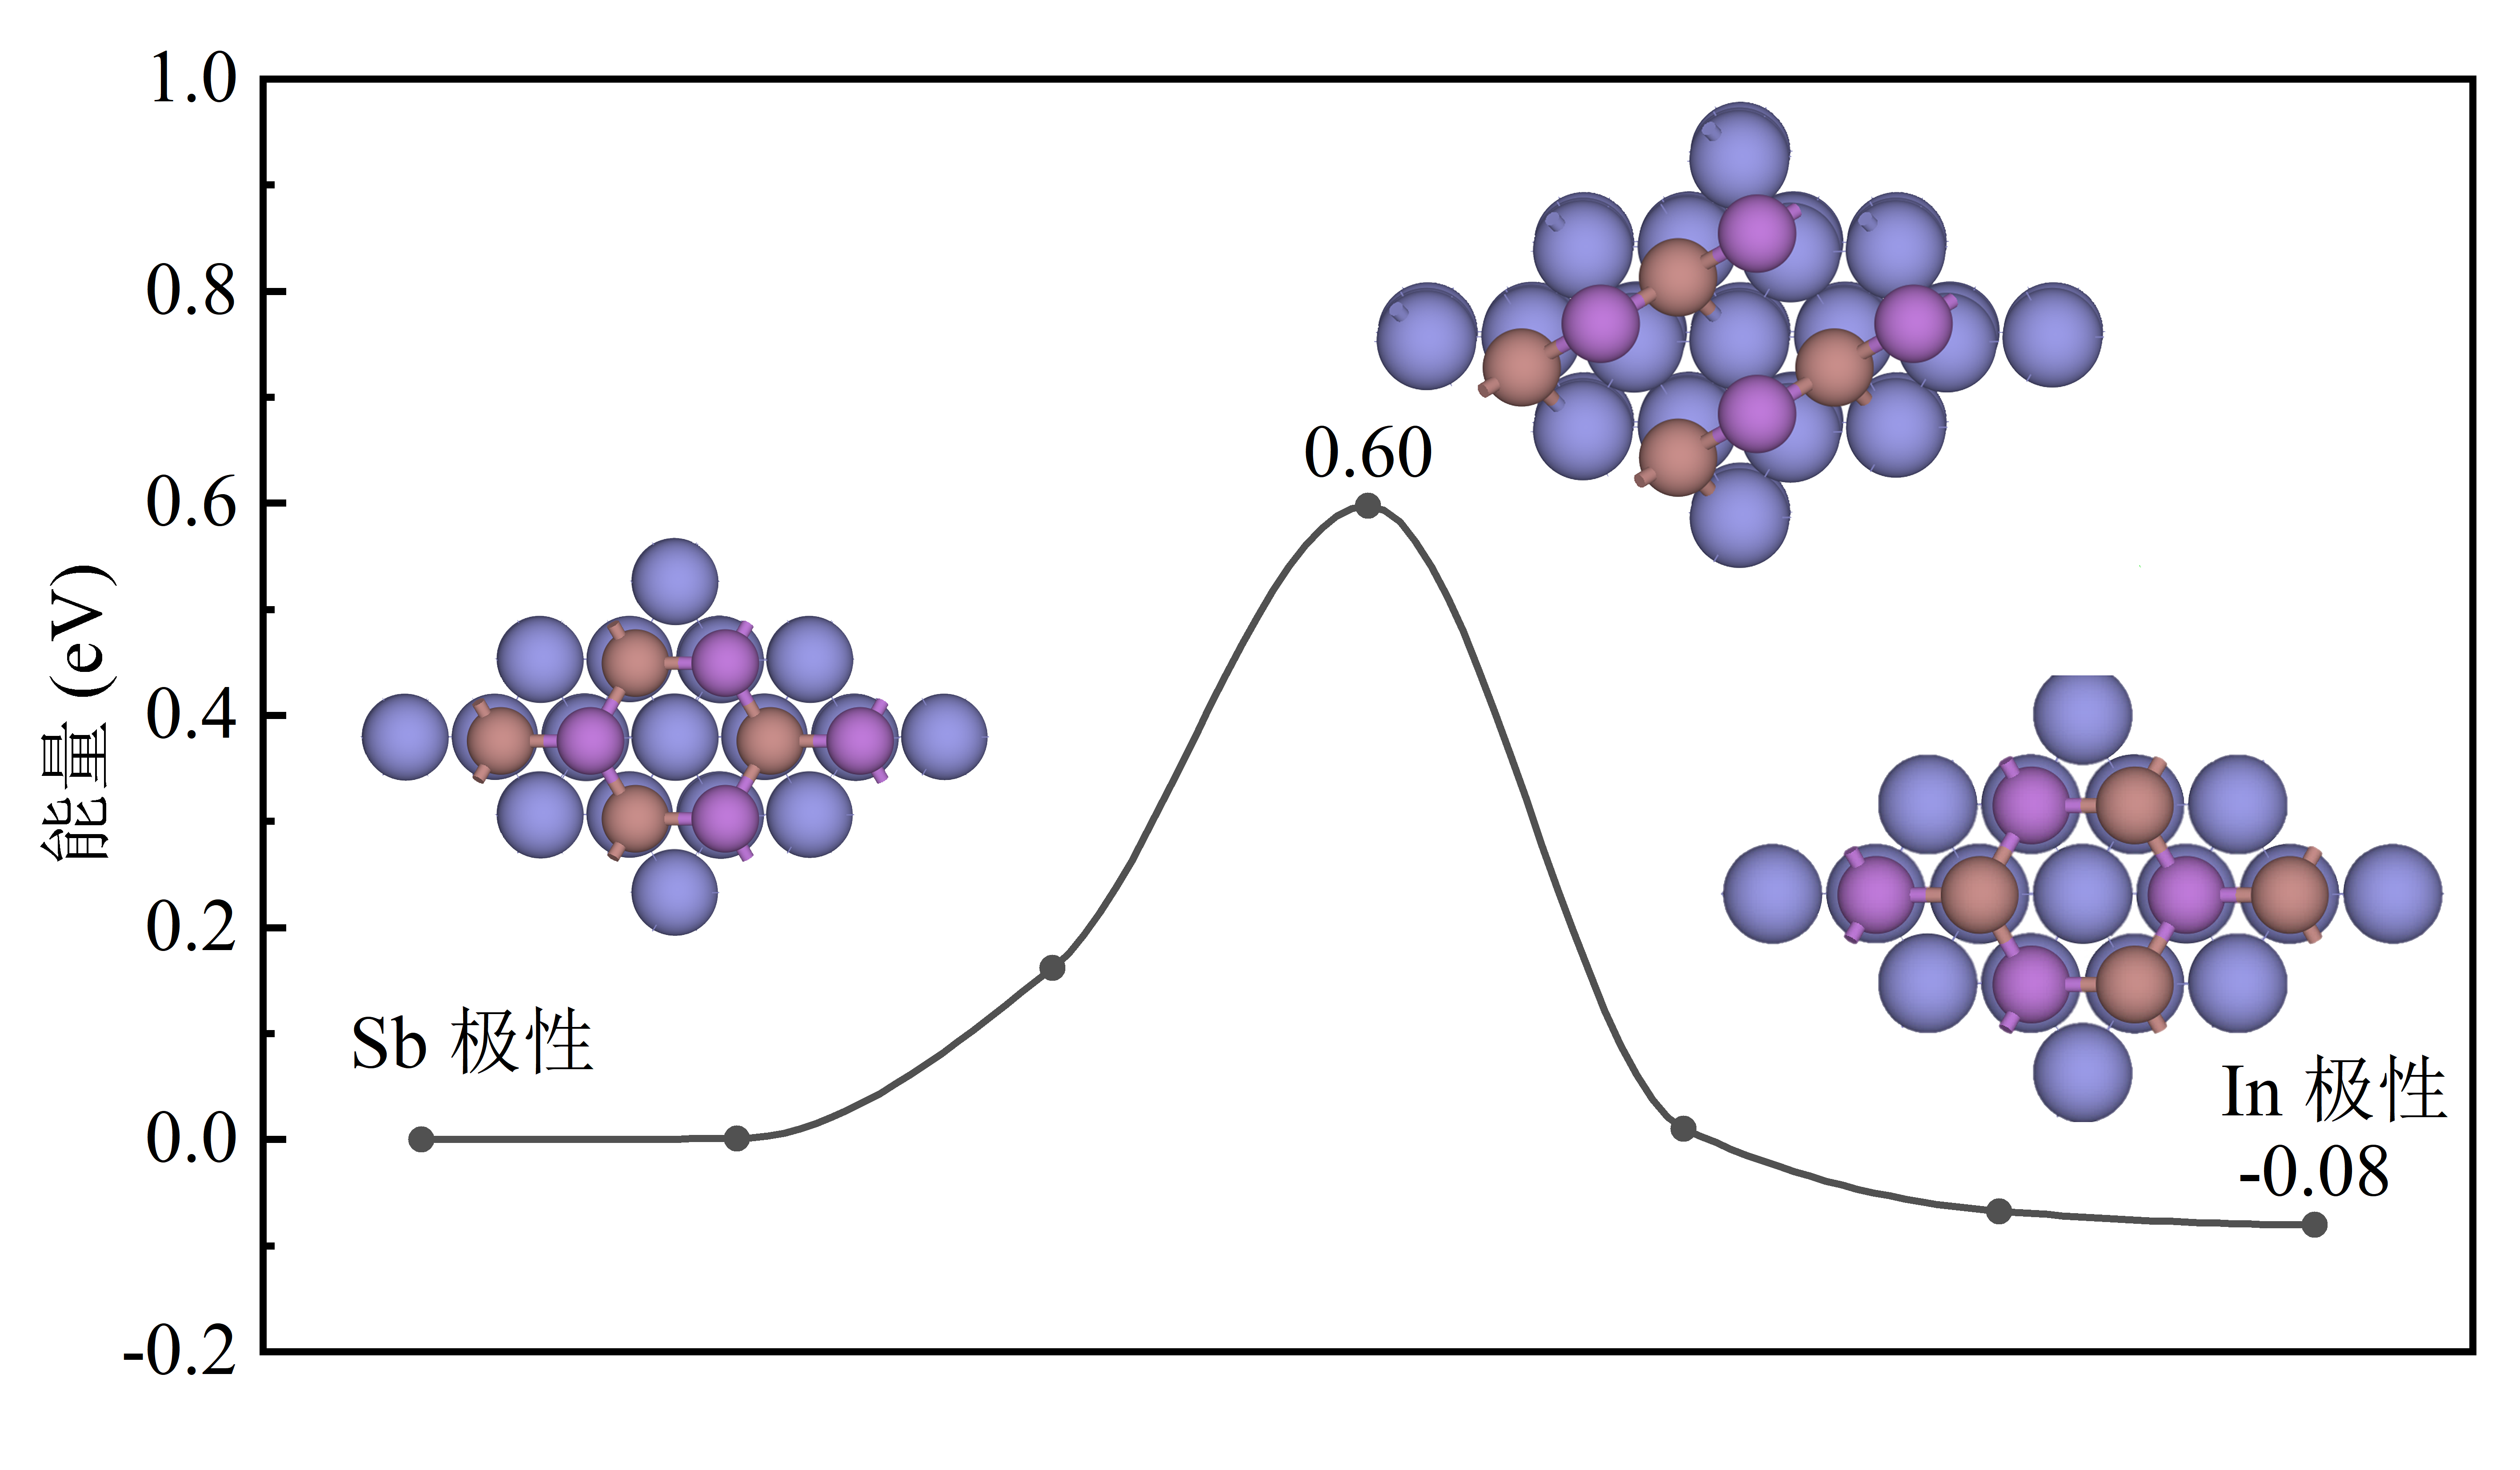
\includegraphics{pic/IS_DFT_1InSb_flipBarrier.png}
    \caption{\cemb{Bi(001)}衬底上单层\cemb{InSb}的极性反转势垒。}
\end{figure}

\section{双层锑化铟的生长机理}
\subsection{双层锑化铟的生长过程}
\begin{figure}[htb]
    \subfloat[]{
        \label{fig:IS_2LInSb_config}
        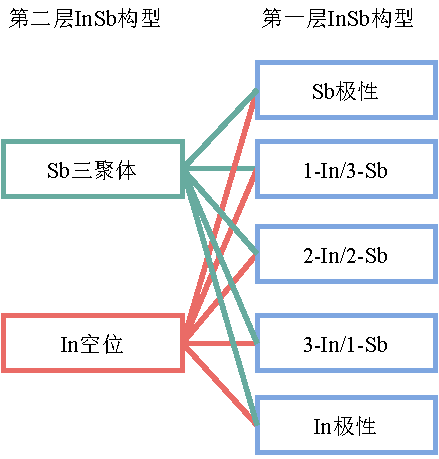
\includegraphics[width=0.48\textwidth]{pic/IS_2LInSb_config.pdf}
    }
    \begin{minipage}[b]{0.5\textwidth}
        \subfloat[]{
            \label{fig:IS_structure_2Linsb_SbT40}
            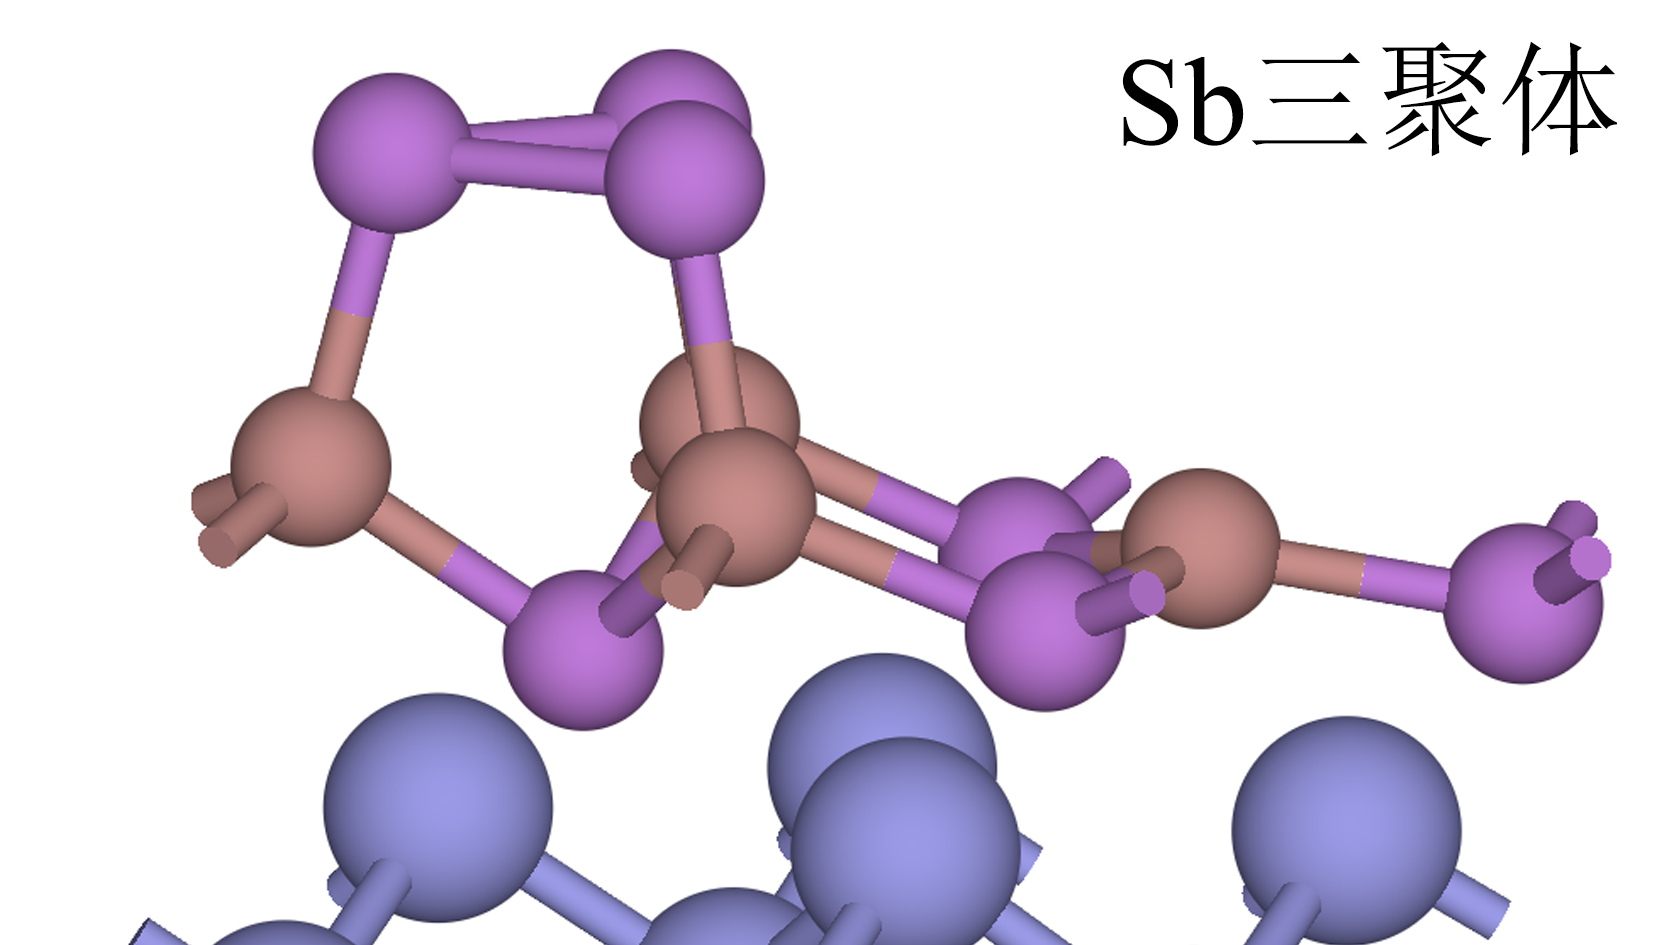
\includegraphics[width=0.8\textwidth]{pic/IS_structure_2Linsb_SbT-40_3Dview.png}
        }
        \newline
        \subfloat[]{
            \label{fig:IS_structure_2Linsb_InV40}
            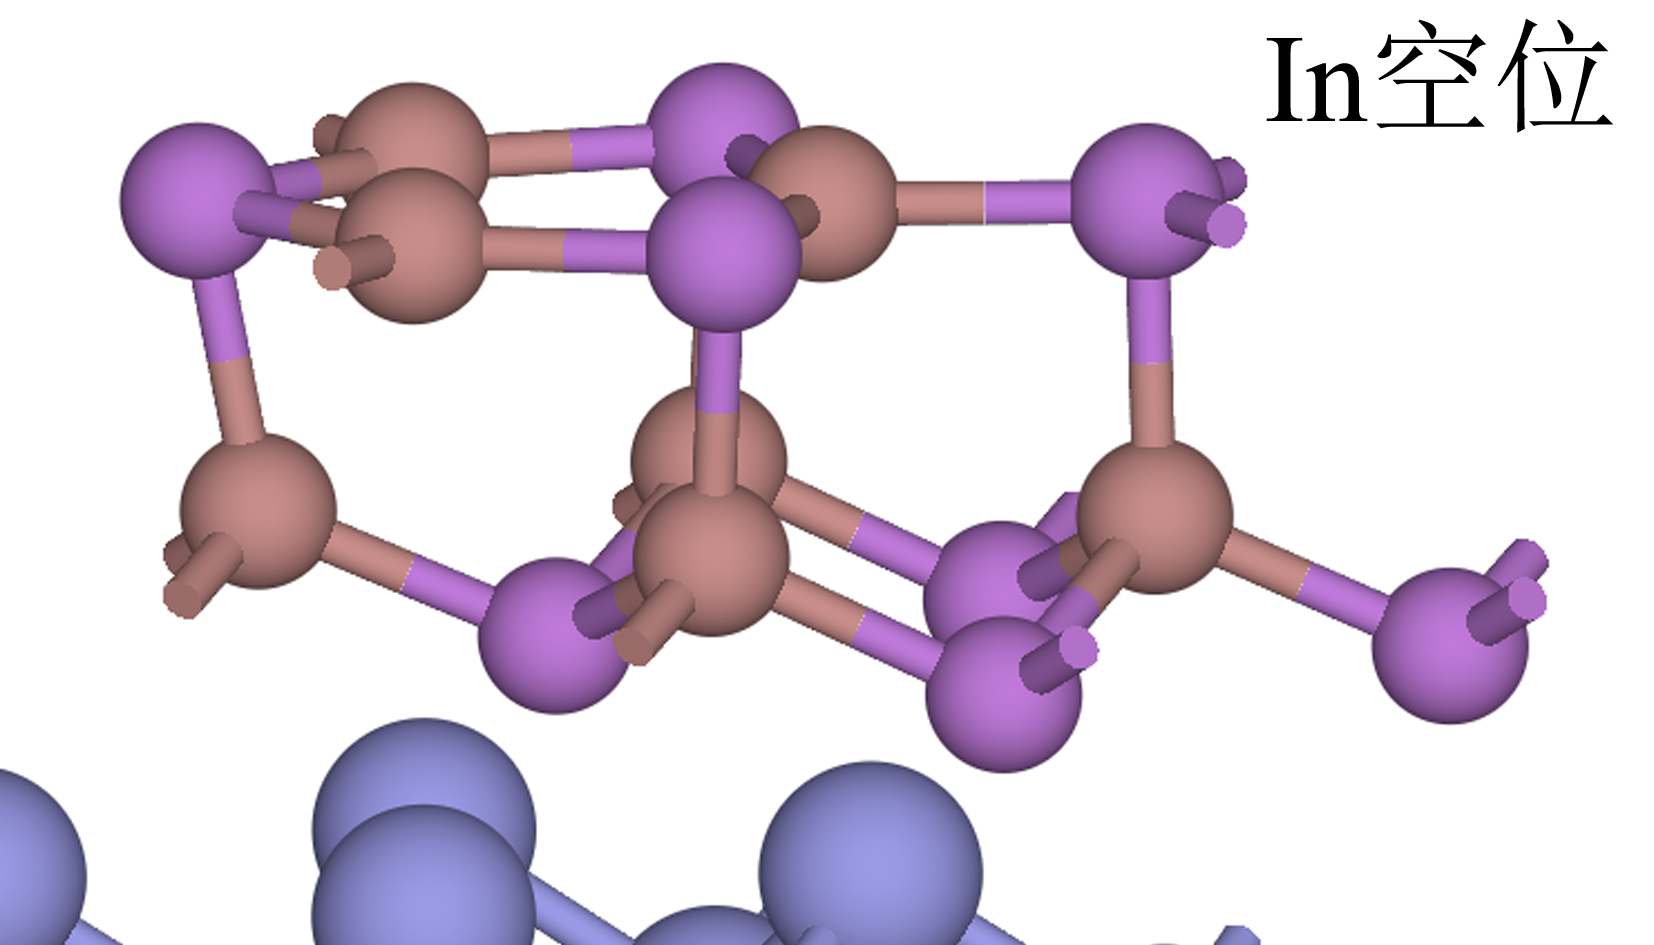
\includegraphics[width=0.8\textwidth]{pic/IS_structure_2Linsb_InV-40_3Dview.png}
        }
    \end{minipage}
    \caption{双层\cemb{InSb}极性极性组合图及原子结构示意图。(a)双层\cemb{InSb}极性极性组合示意图;(b)双层\cemb{InSb}原子结构,\cemb{Sb}三聚体第二层覆盖\cemb{In}极性第一层;(b)双层\cemb{InSb}原子结构,\cemb{In}空位第二层覆盖\cemb{In}极性第一层。}
    \label{fig:IS_structure_2Linsb}
\end{figure}

\begin{figure}[htb]
    \subfloat[]{
        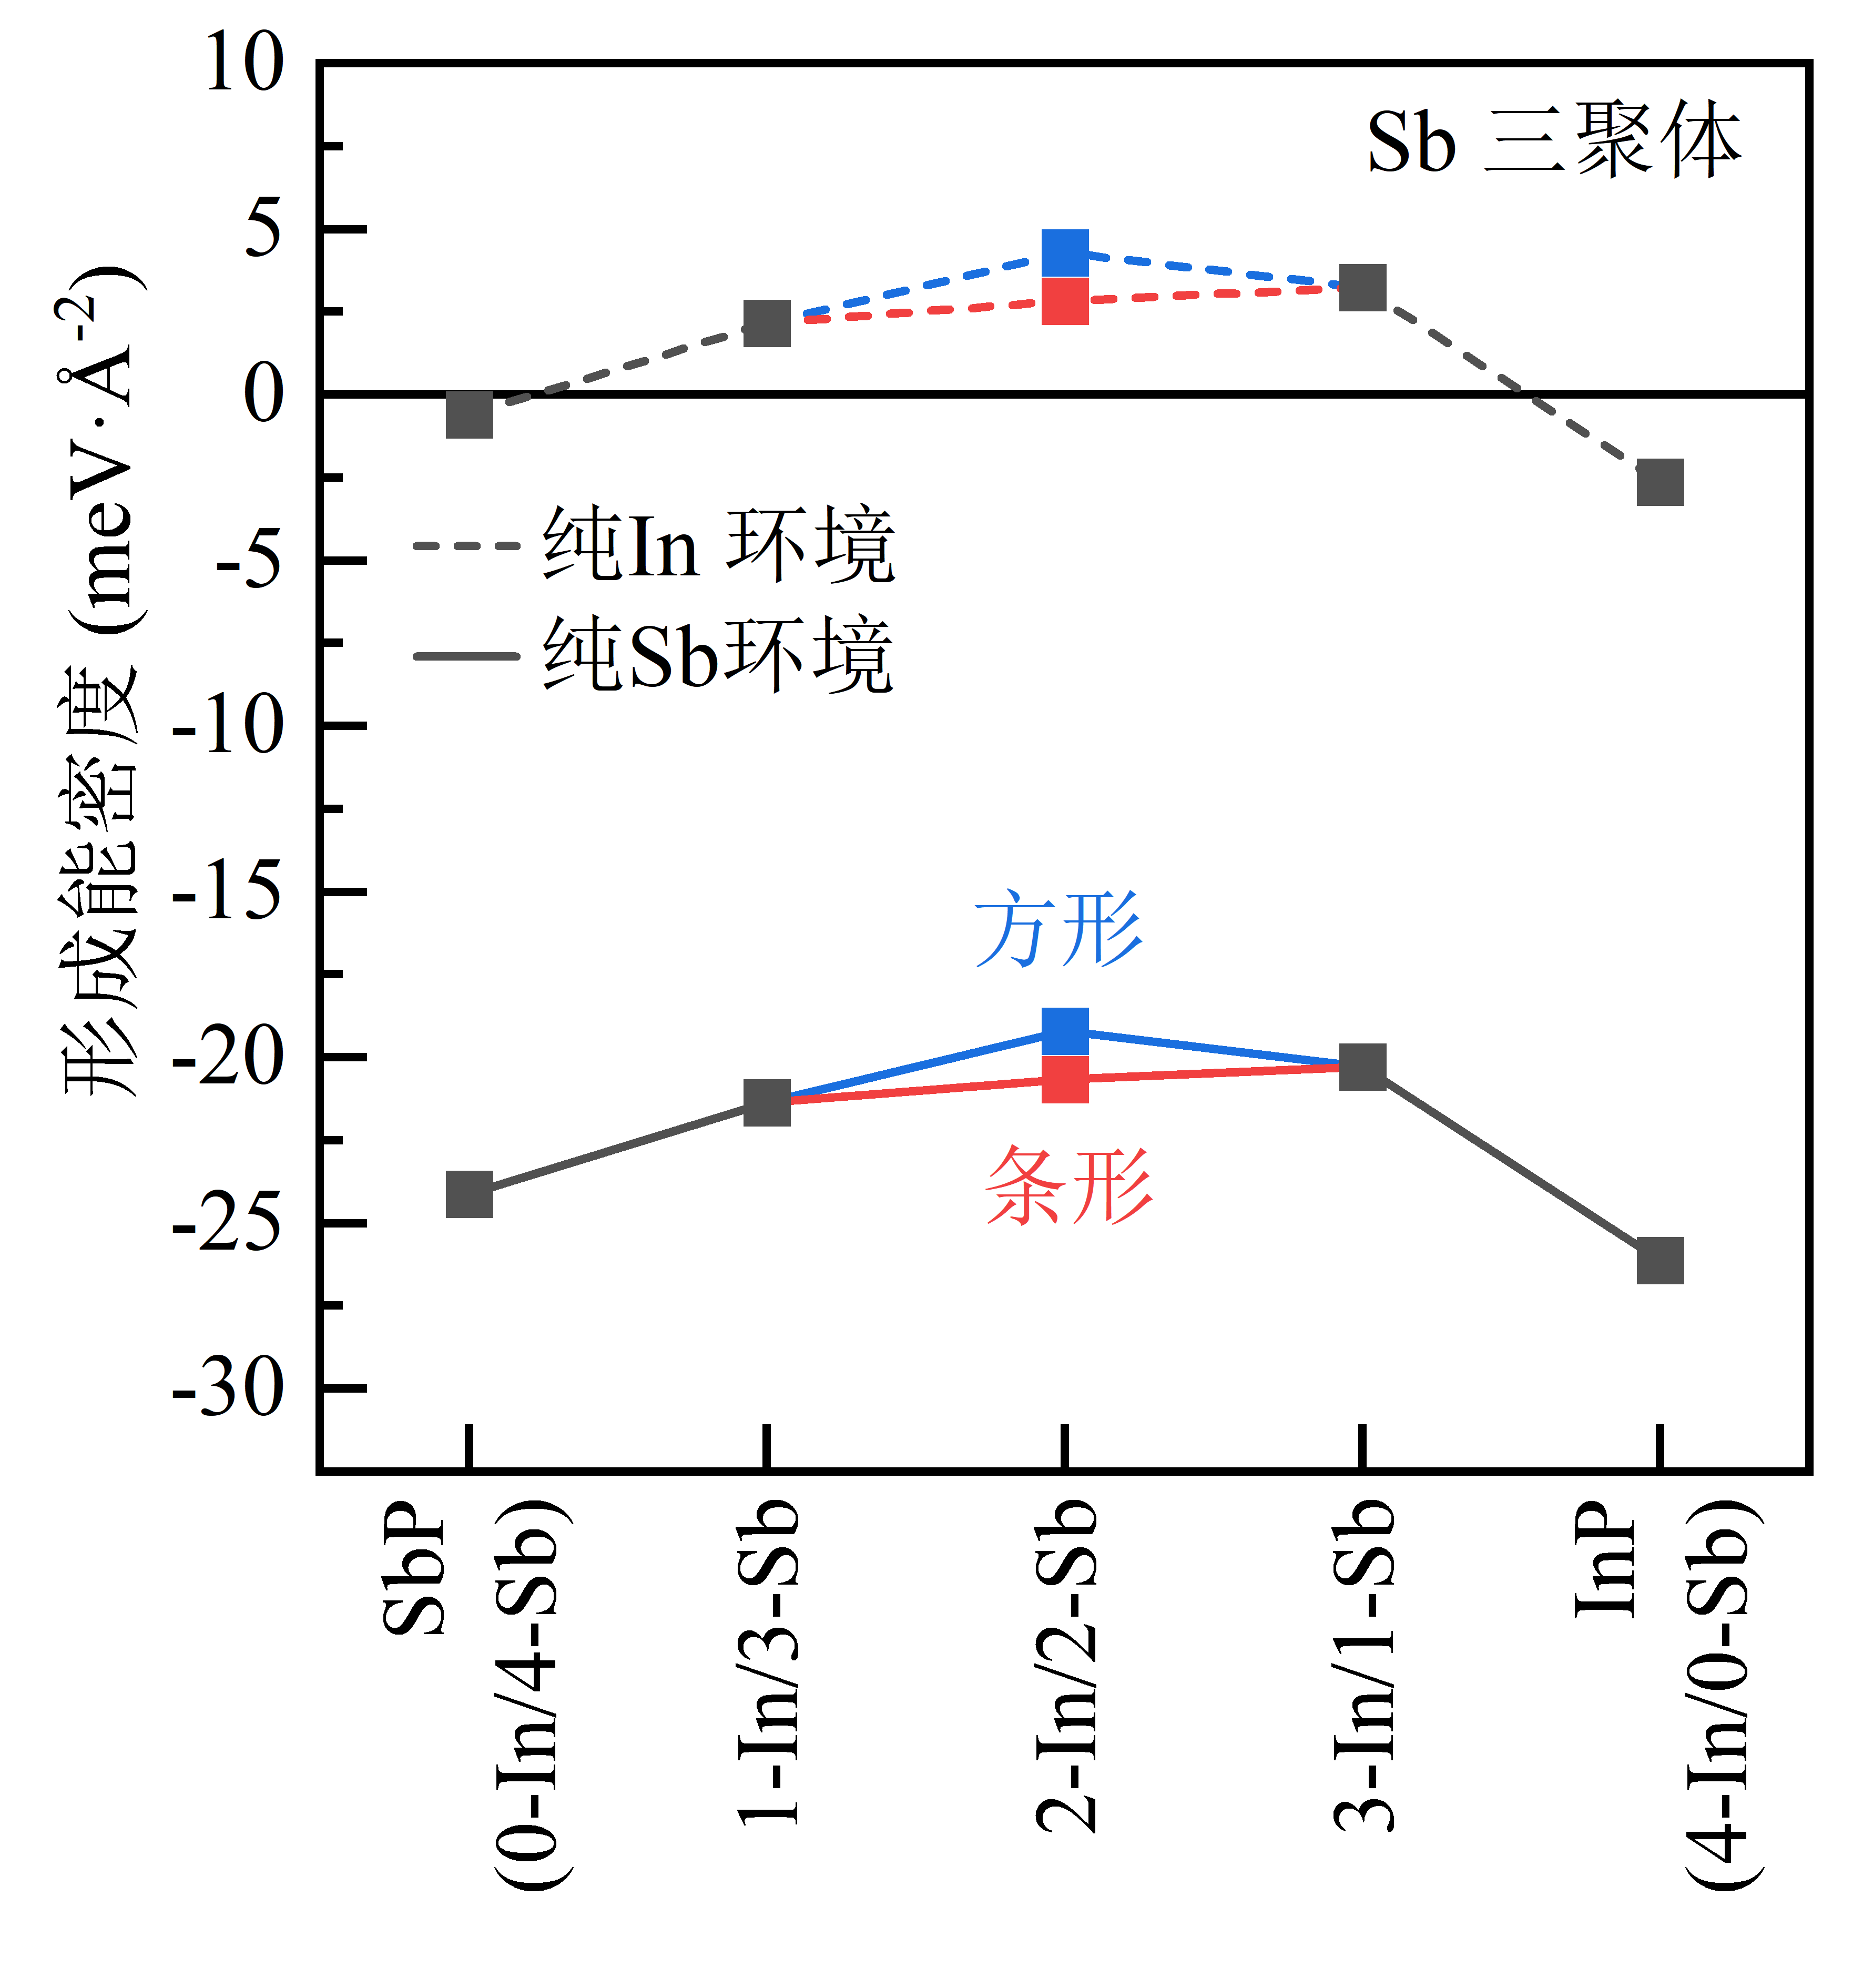
\includegraphics[width=0.45\textwidth]{pic/IS_DFT_2LInSb_SbTonAll.png}
        \label{IS_DFT_2LInSb_SbTonAll}
    }
    \subfloat[]{
        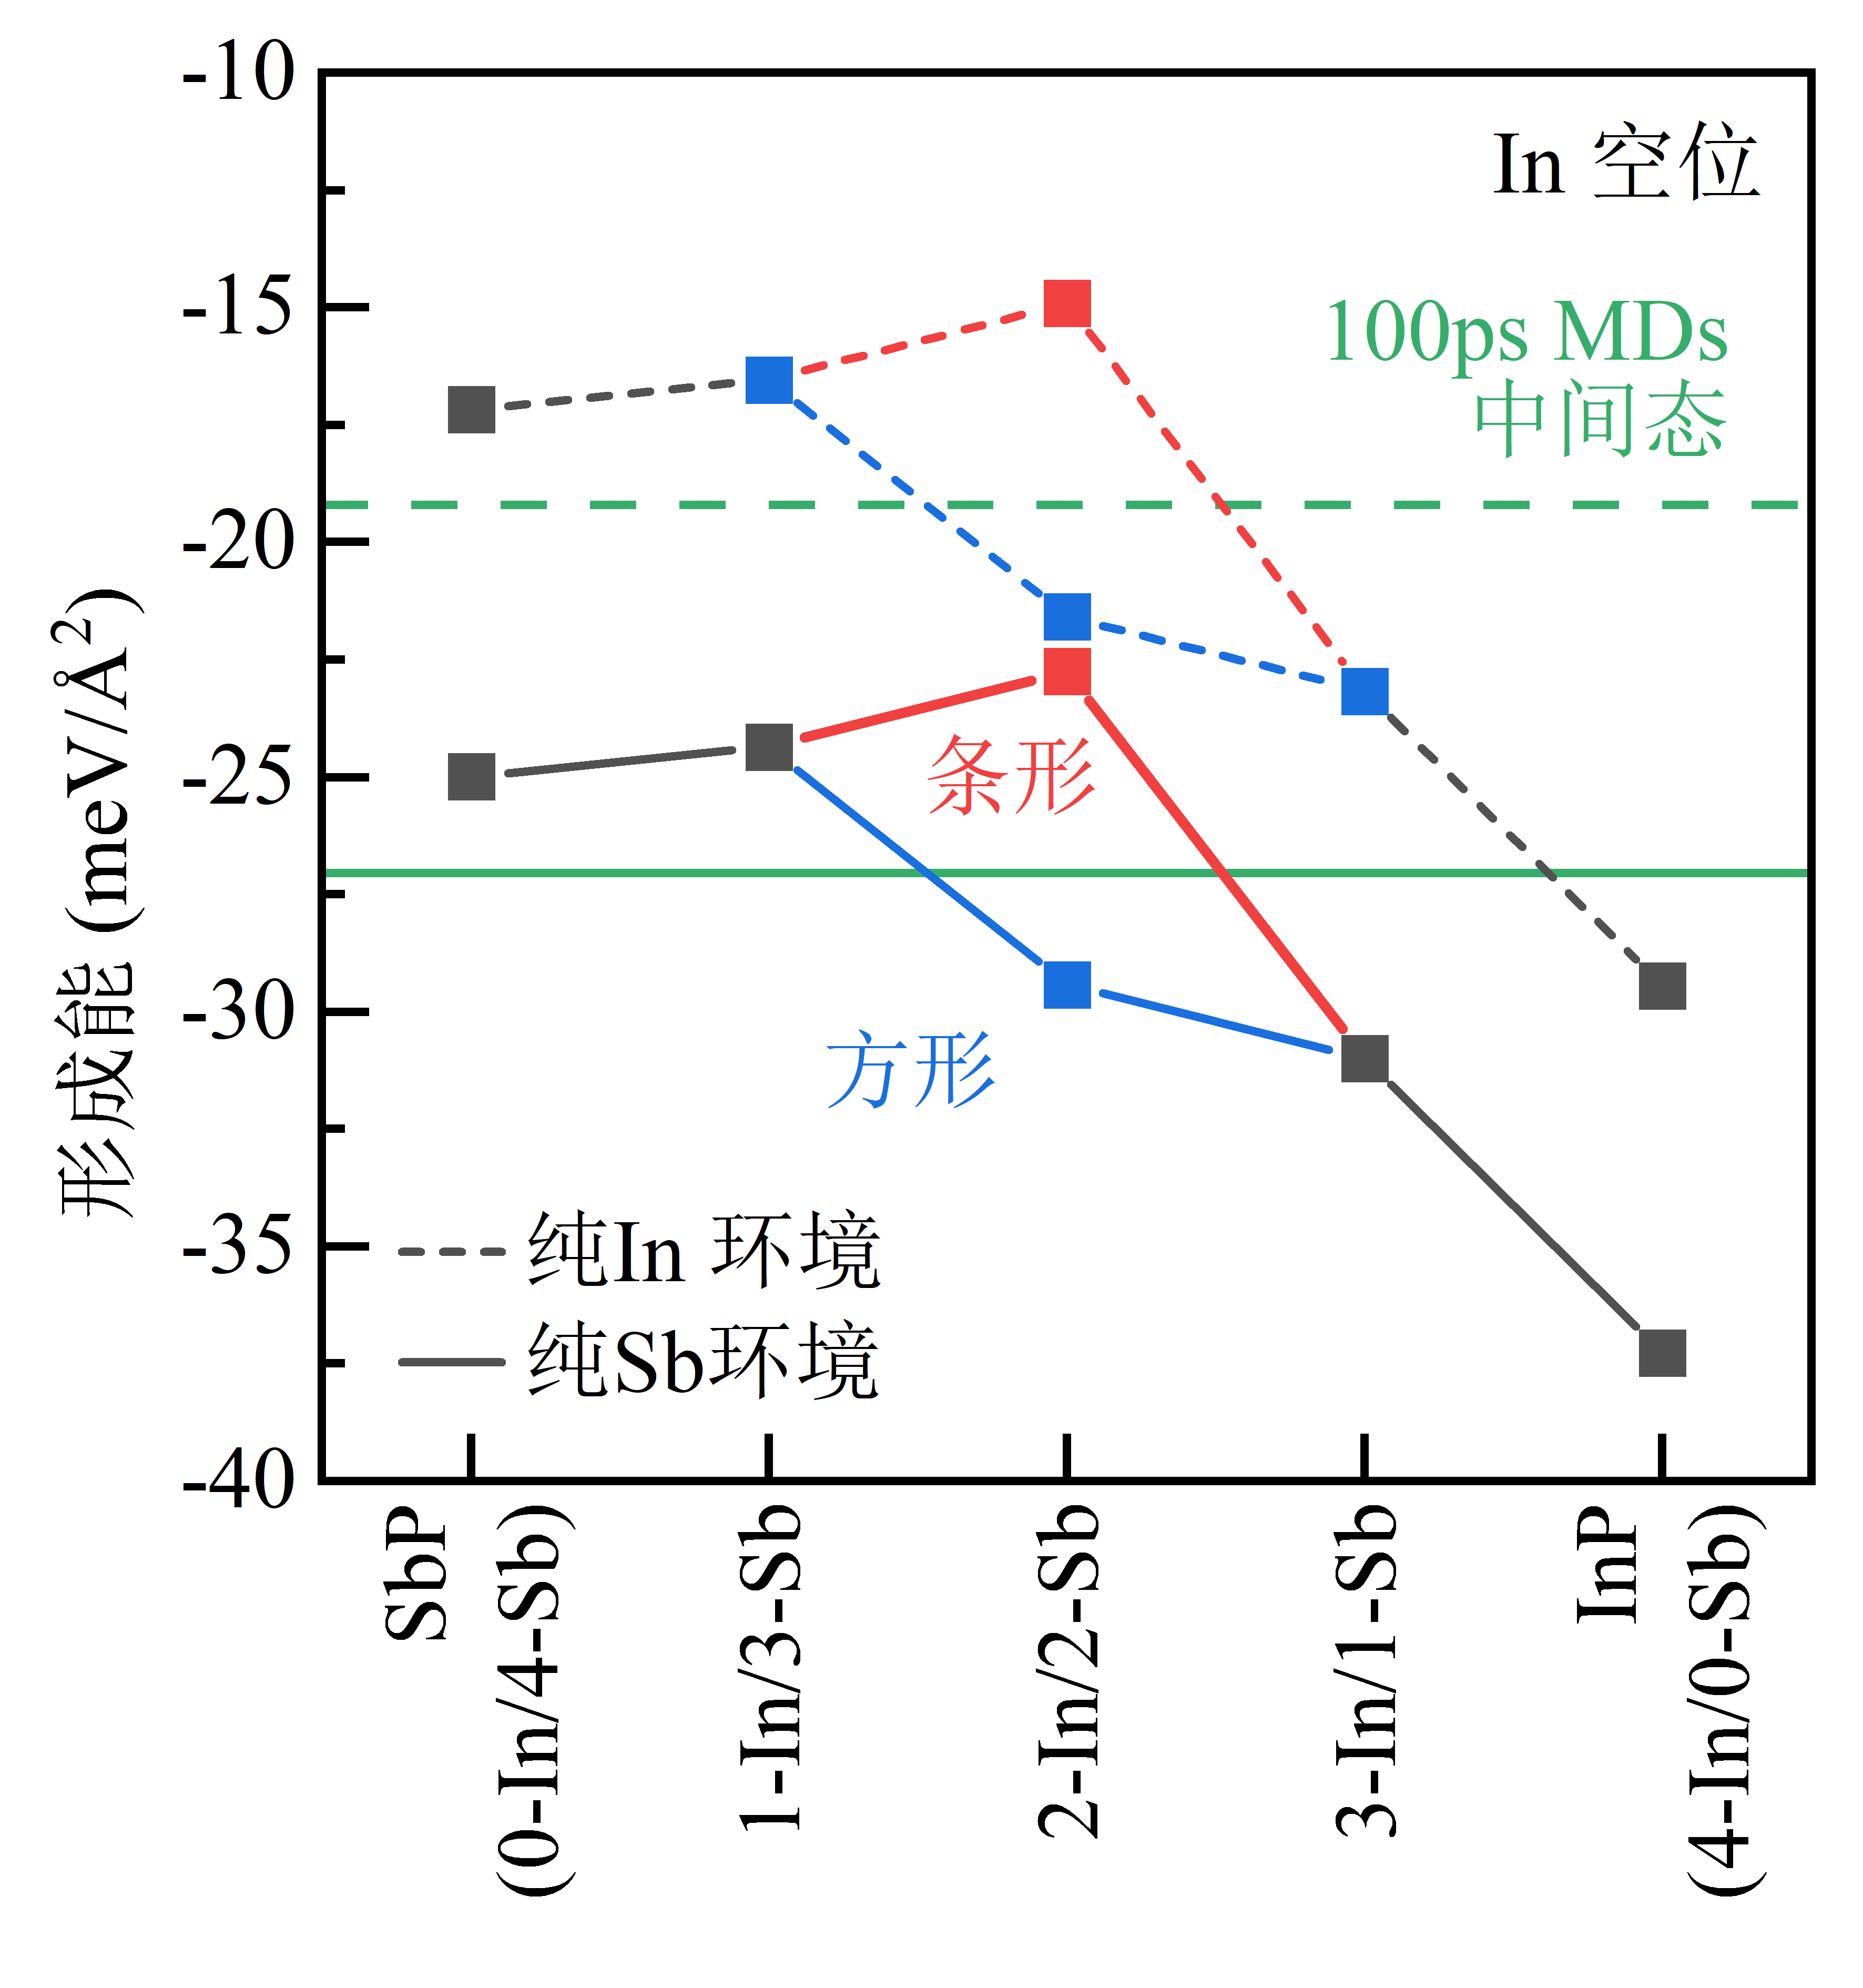
\includegraphics[width=0.45\textwidth]{pic/IS_DFT_2LInSb_InVonAll.png}
        \label{IS_DFT_2LInSb_InVonAll}
    }
    \caption{\cemb{Bi(001)}衬底上双层\cemb{InSb}的形成能分布。(a)以Sb三聚体为第二层的双层\cemb{InSb}的形成能分布;(b)以In空位层为第二层的双层\cemb{InSb}的形成能分布。}
    \label{fig:IS_DFT_2LInSb_formationEnergy}
\end{figure}

\begin{figure}
    \subfloat[]{
        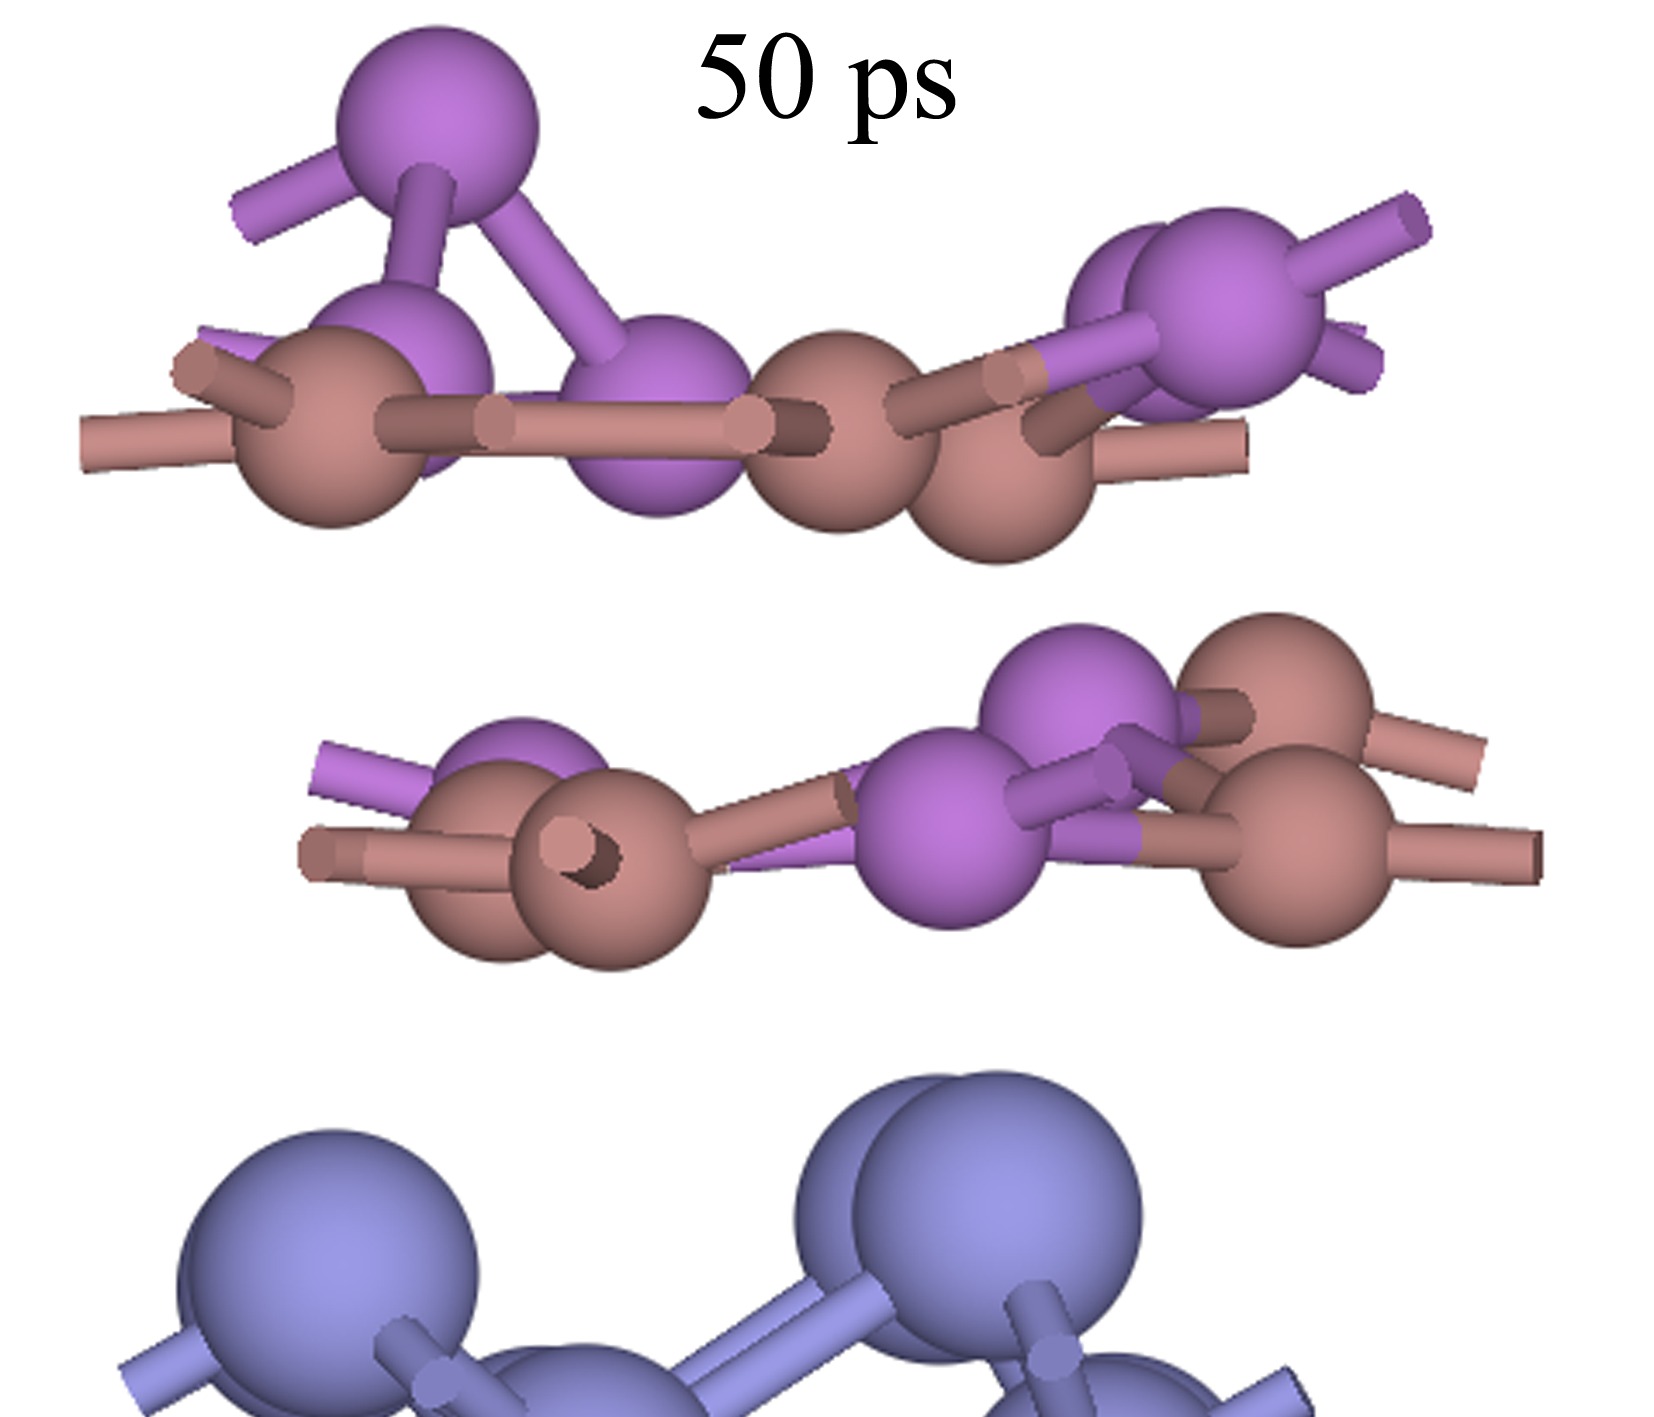
\includegraphics{pic/IS_structure_2Linsb_md50ps.png}
        \label{fig:IS_structure_2Linsb_md50ps}
    }
    \subfloat[]{
        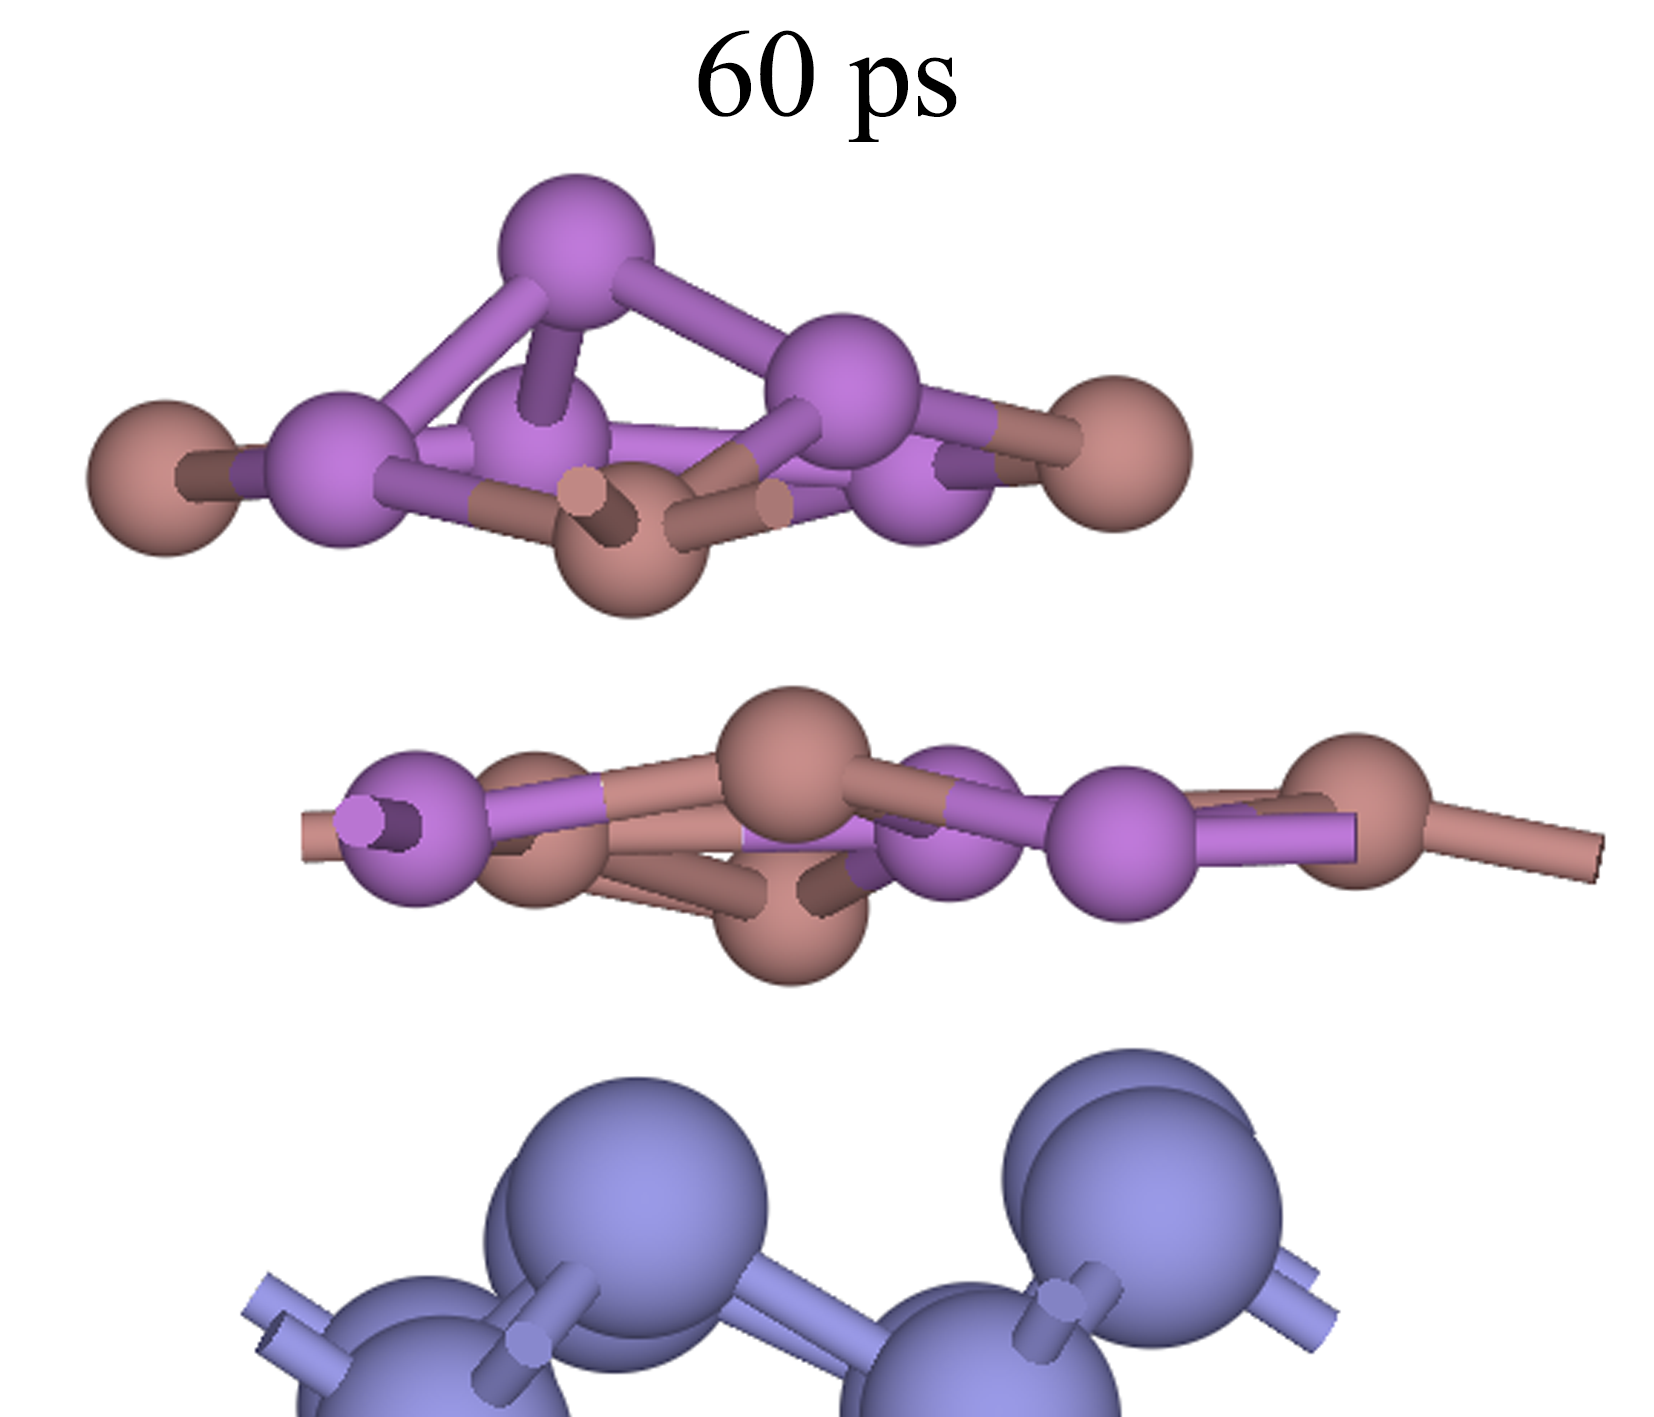
\includegraphics{pic/IS_structure_2Linsb_md60ps.png}
        \label{fig:IS_structure_2Linsb_md60ps}
    }\\[-0.5ex]
    \subfloat[]{
        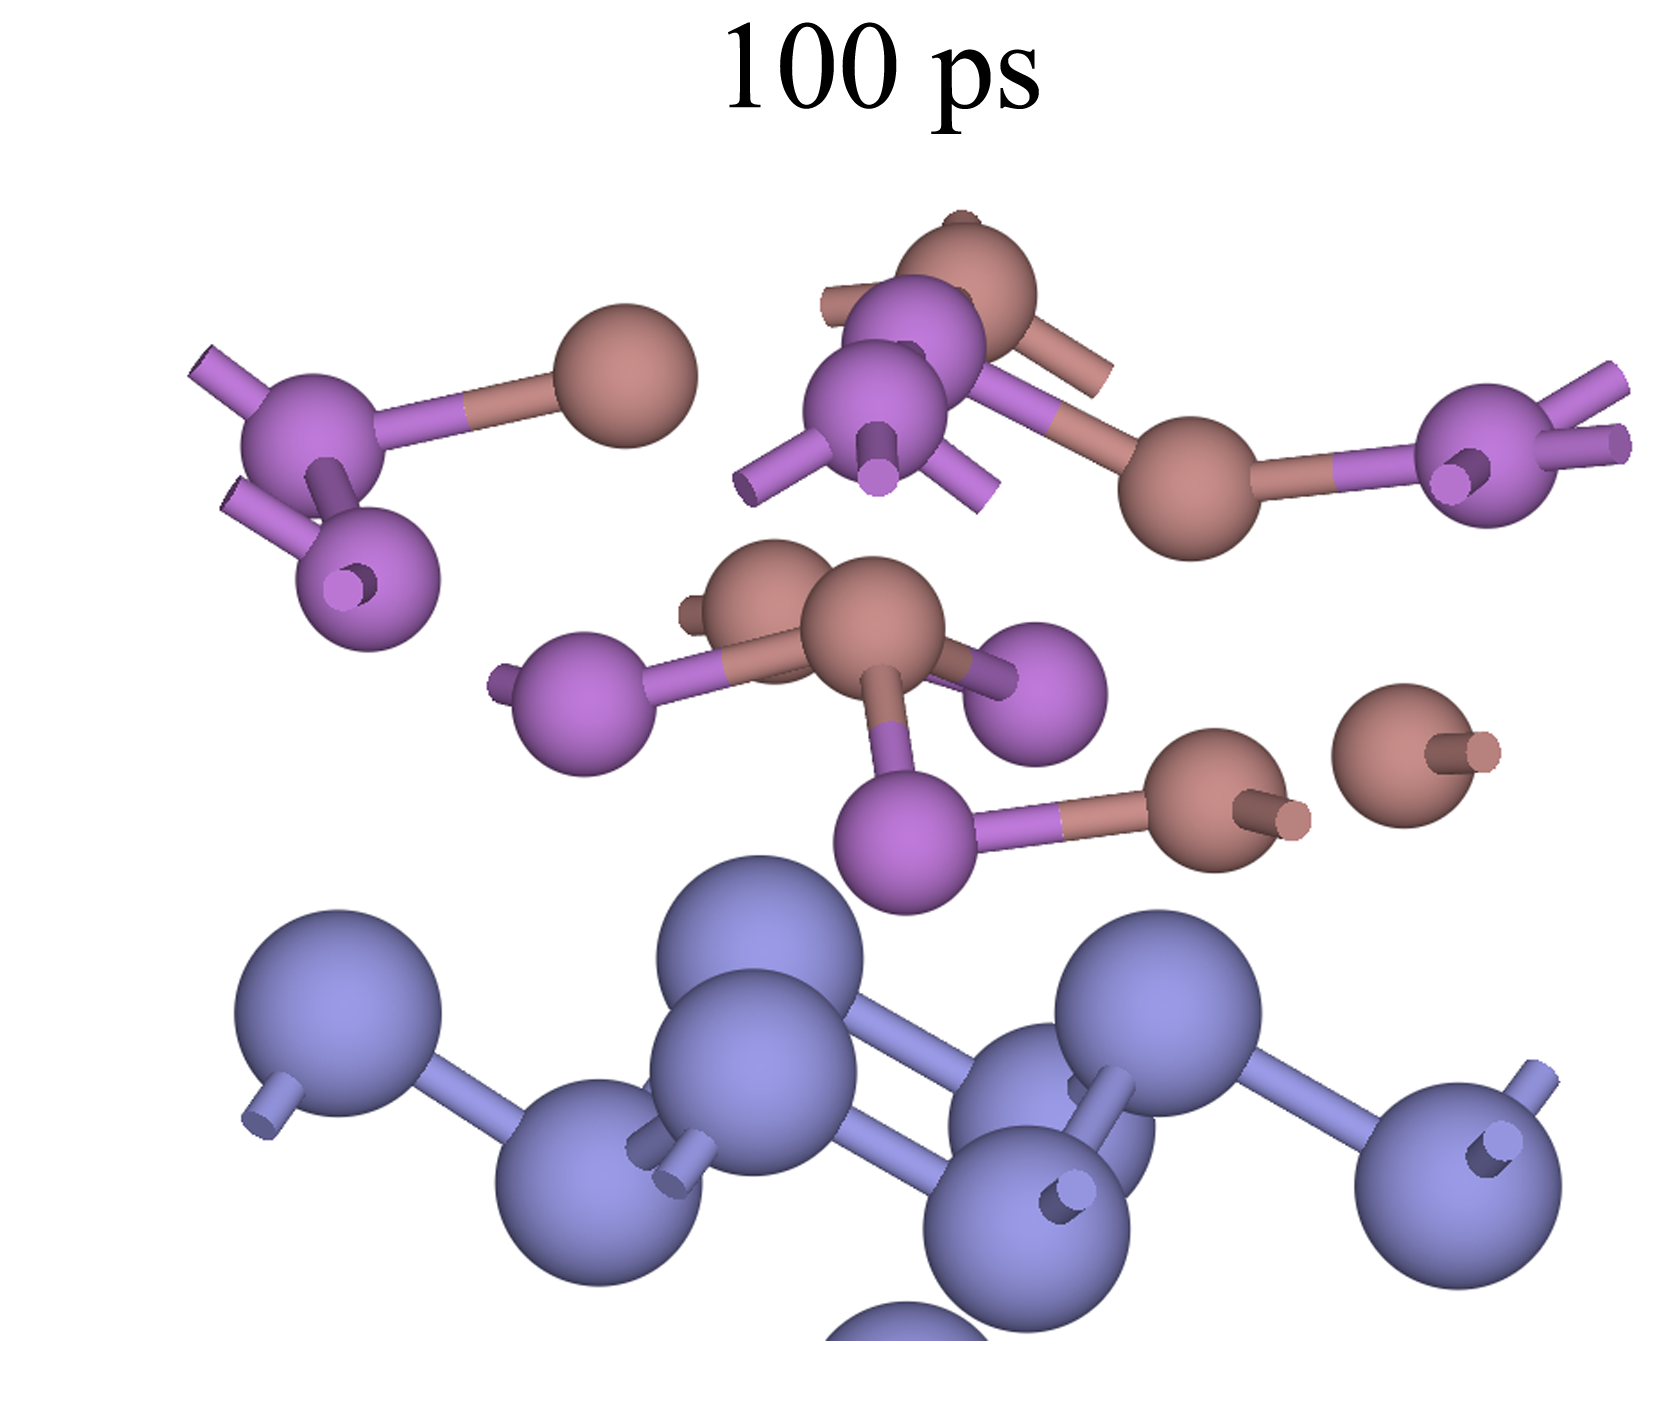
\includegraphics{pic/IS_structure_2Linsb_md100ps.png}
        \label{fig:IS_structure_2Linsb_md100ps}
    }
    \subfloat[]{
        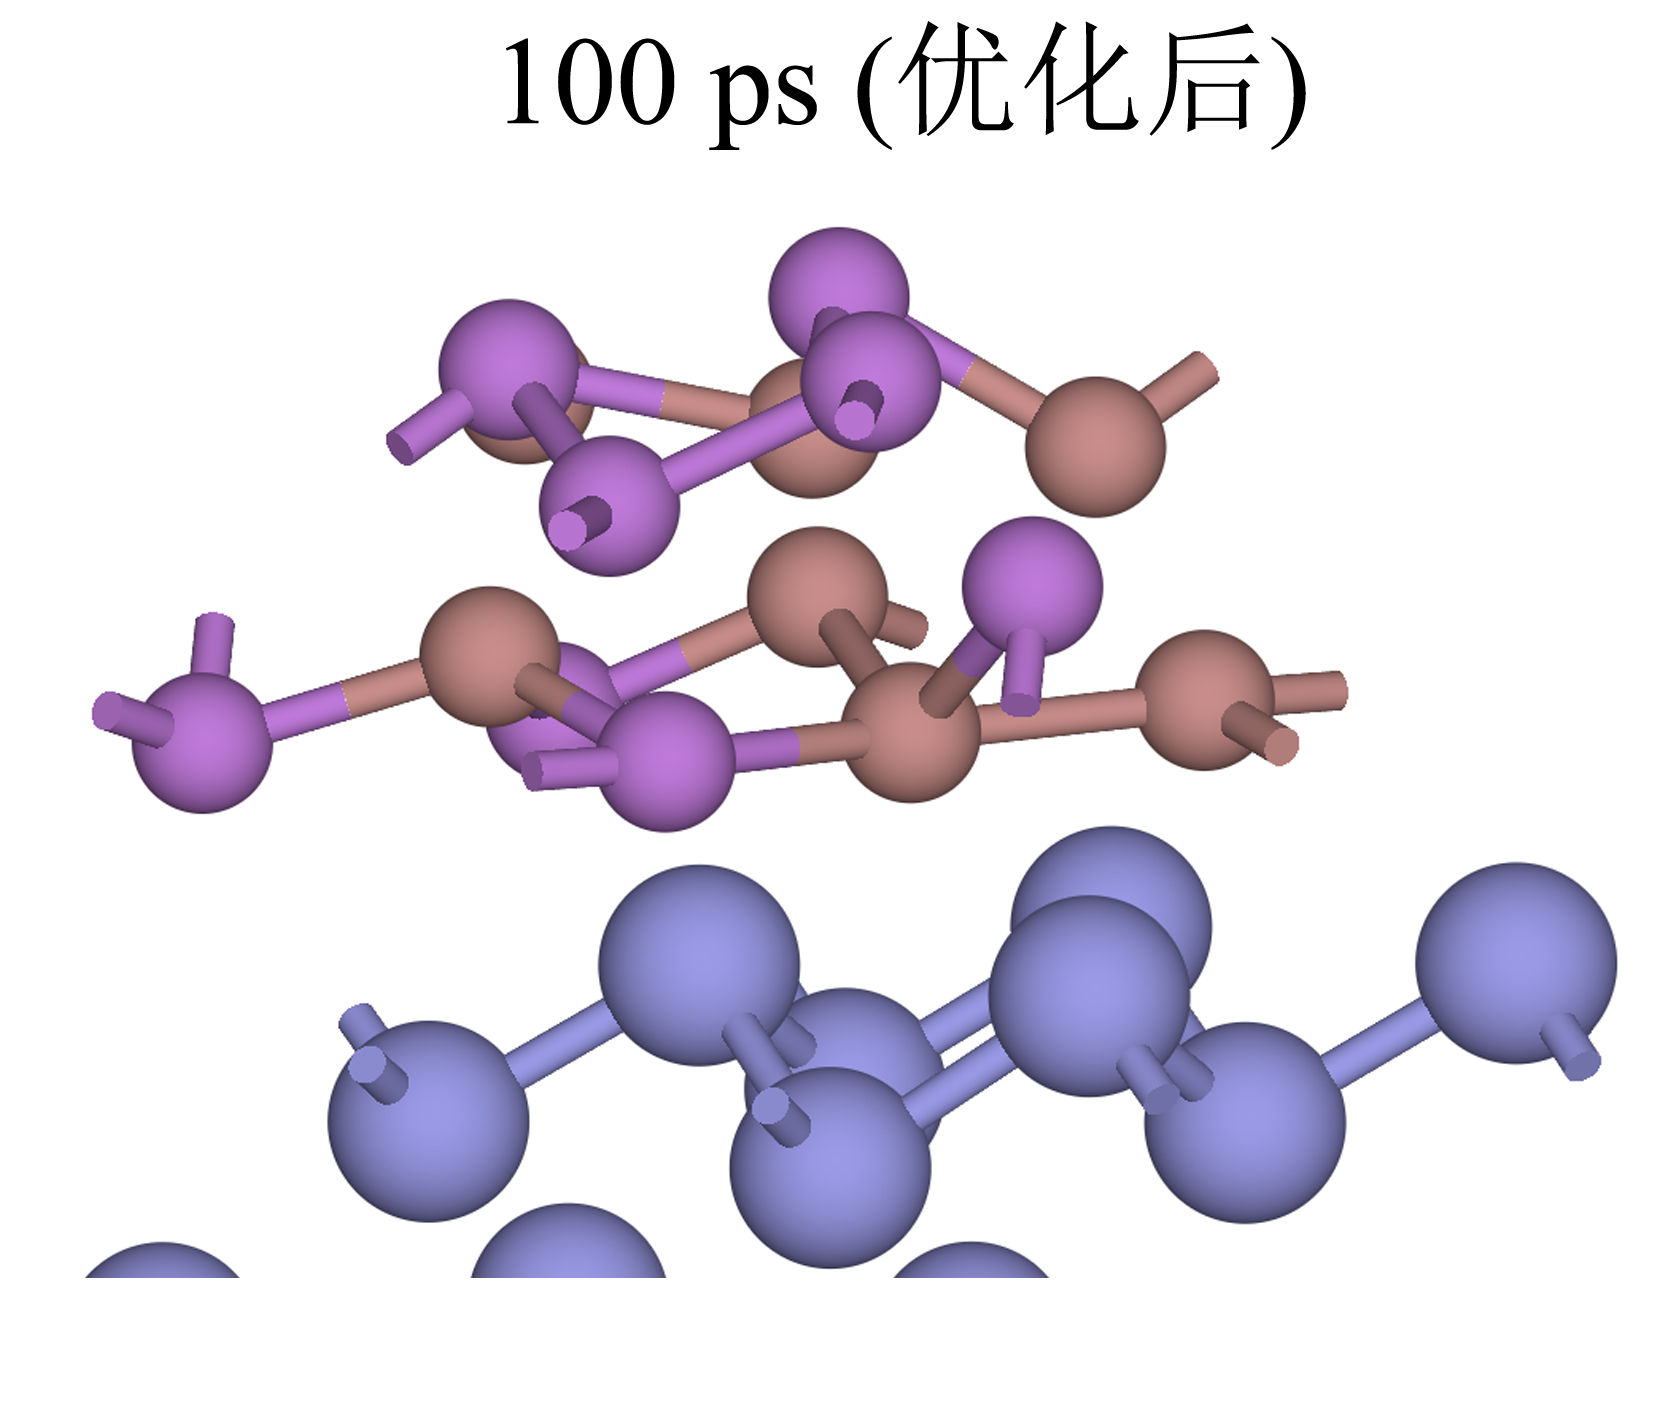
\includegraphics{pic/IS_structure_2Linsb_md100psopt.png}
        \label{fig:IS_structure_2Linsb_md100psopt}
    }
    \caption{\cemb{Bi(001)}衬底上双层\cemb{InSb}极性演化的分子动力学模拟结果。(a)分子动力学模拟50ps后的原子结构图;(b)分b动力学模拟60ps后的原子结构图;(c)分子动力学模拟100ps后的原子结构图;(d)100ps对应中间态的原子结构图。}
    \label{fig:IS_structure_2Linsb_md}
\end{figure}

\begin{figure}
    \subfloat[]{
        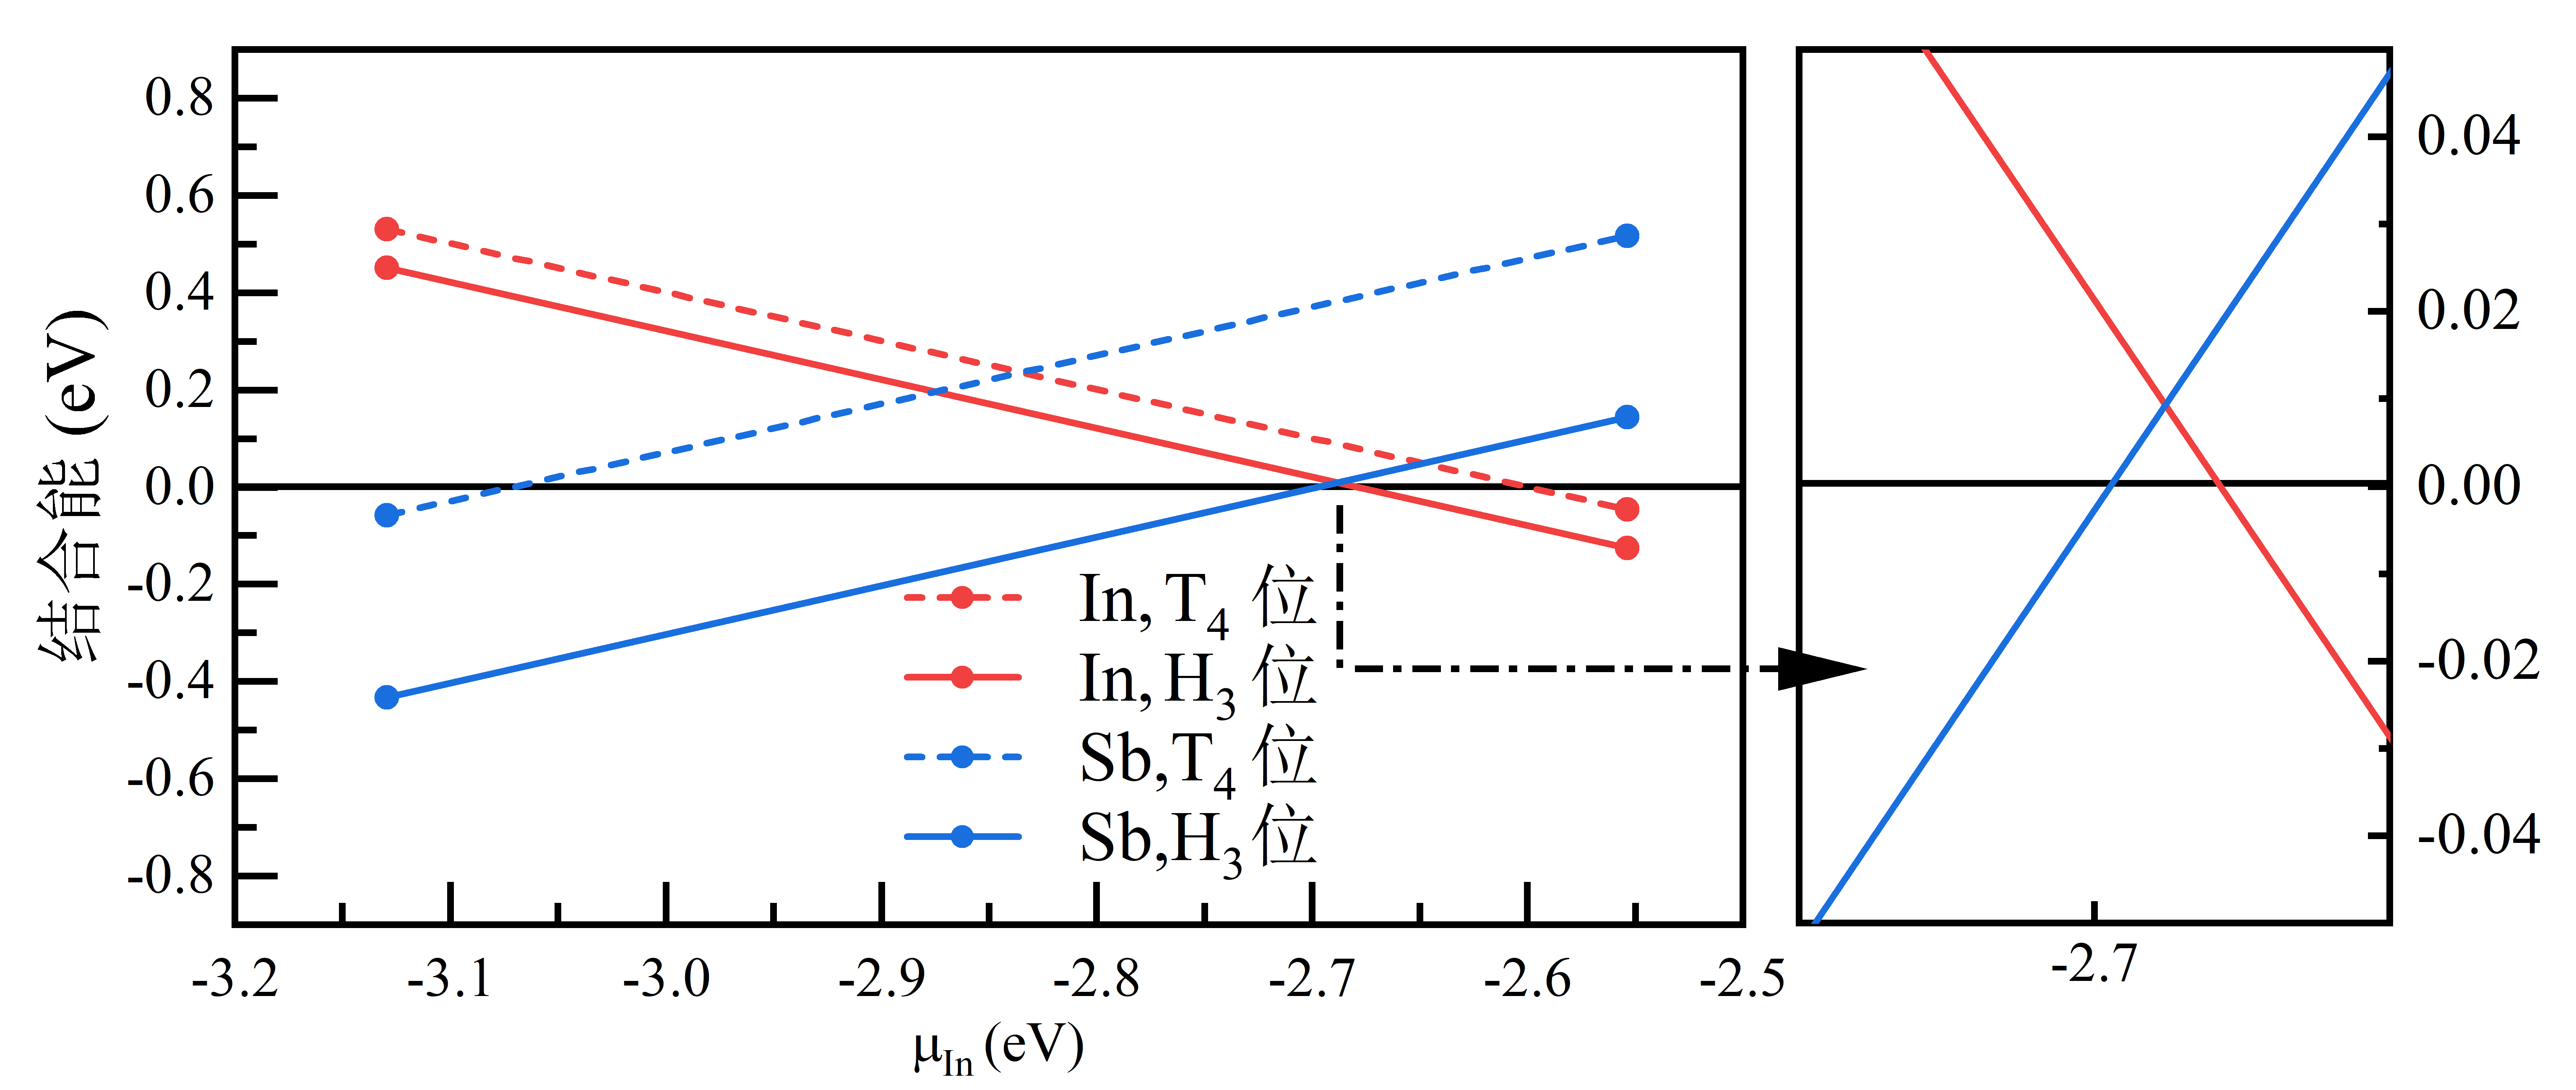
\includegraphics{pic/IS_DFT_2InSb_adatoms.png}
    }\\[-0.5ex]
    \subfloat[]{
        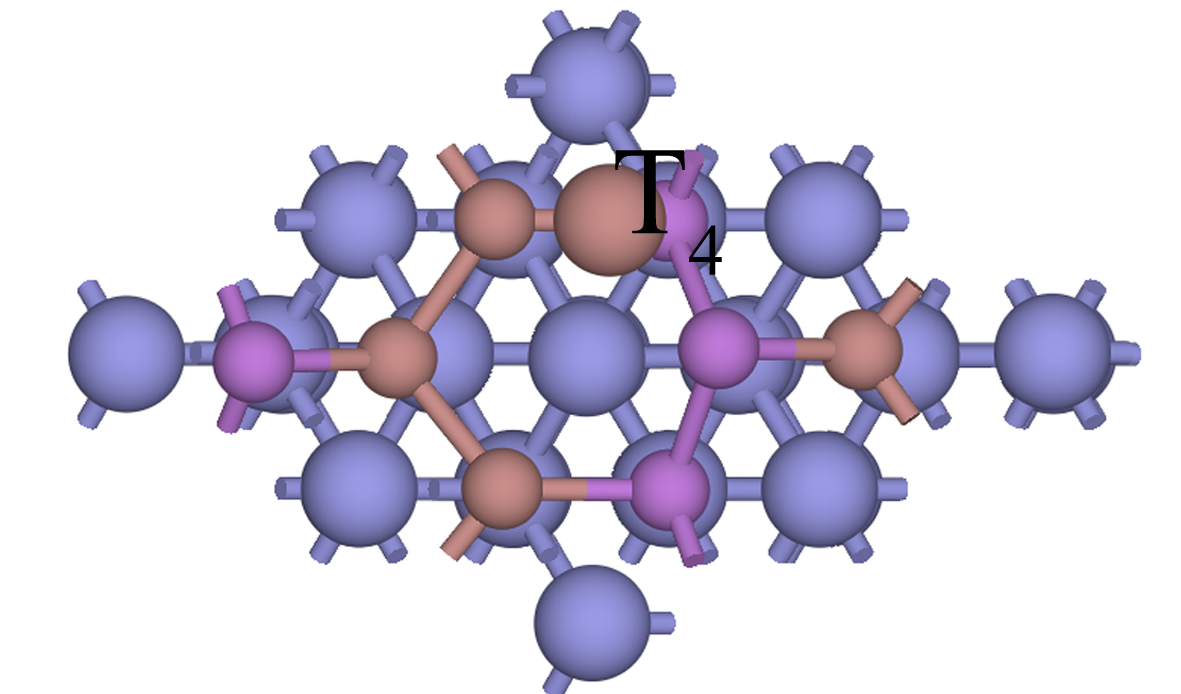
\includegraphics{pic/IS_structure_2Linsb_adatoms_InT4.png}
    }
    \subfloat[]{
        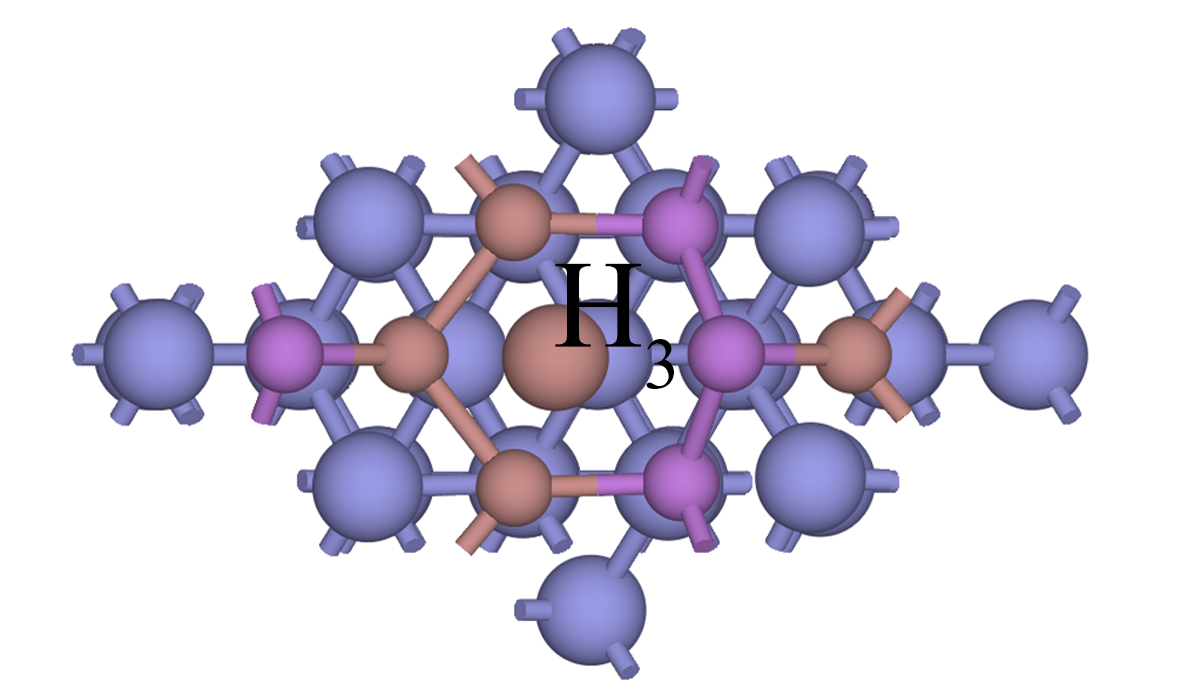
\includegraphics{pic/IS_structure_2Linsb_adatoms_InH3.png}
    }\\[-0.5ex]
    \subfloat[]{
        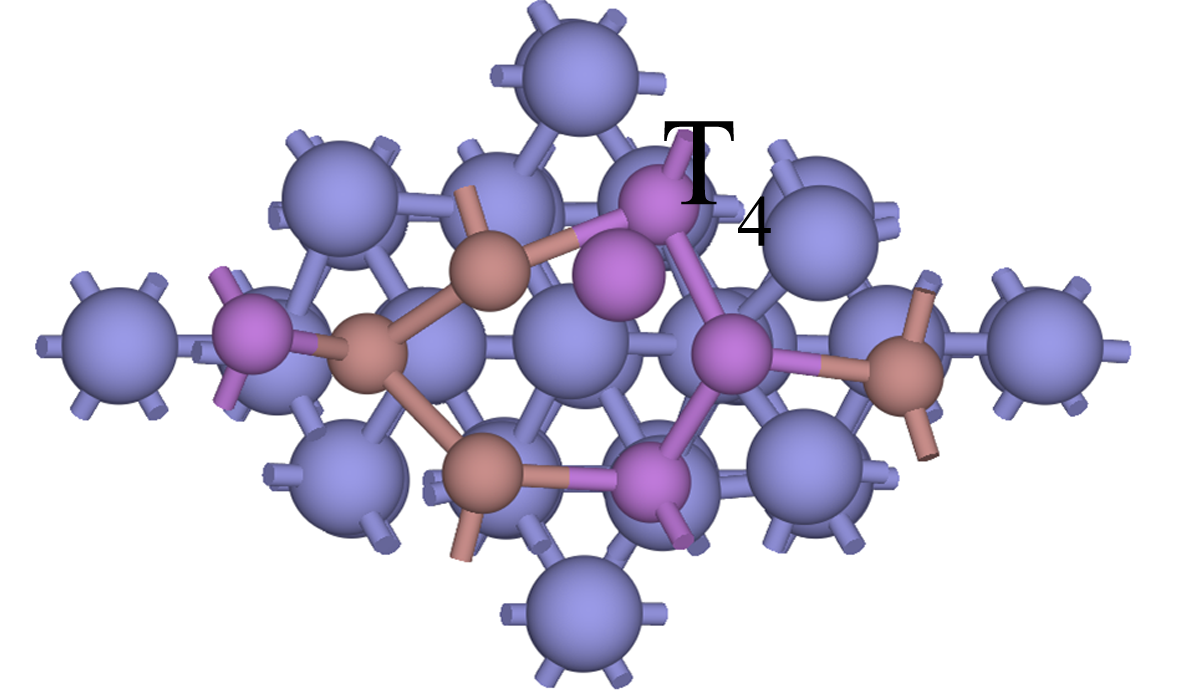
\includegraphics{pic/IS_structure_2Linsb_adatoms_SbT4.png}
    }
    \subfloat[]{
        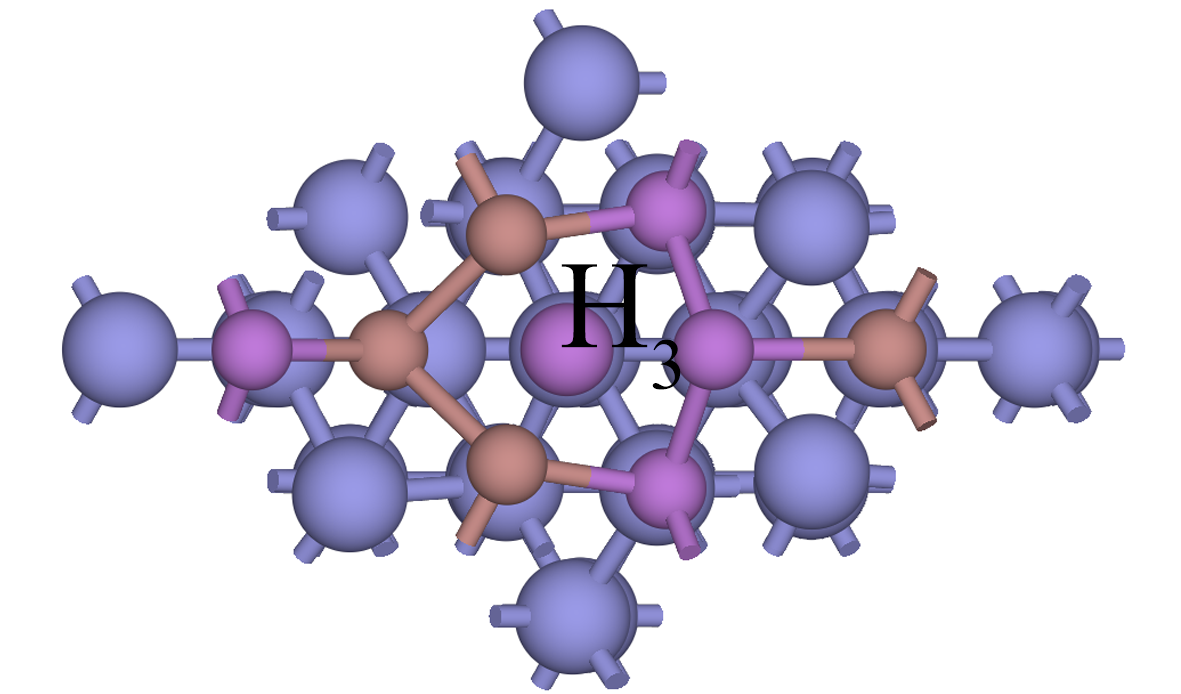
\includegraphics{pic/IS_structure_2Linsb_adatoms_SbH3.png}
    }
\end{figure}

\begin{figure}
    \subfloat[]{
        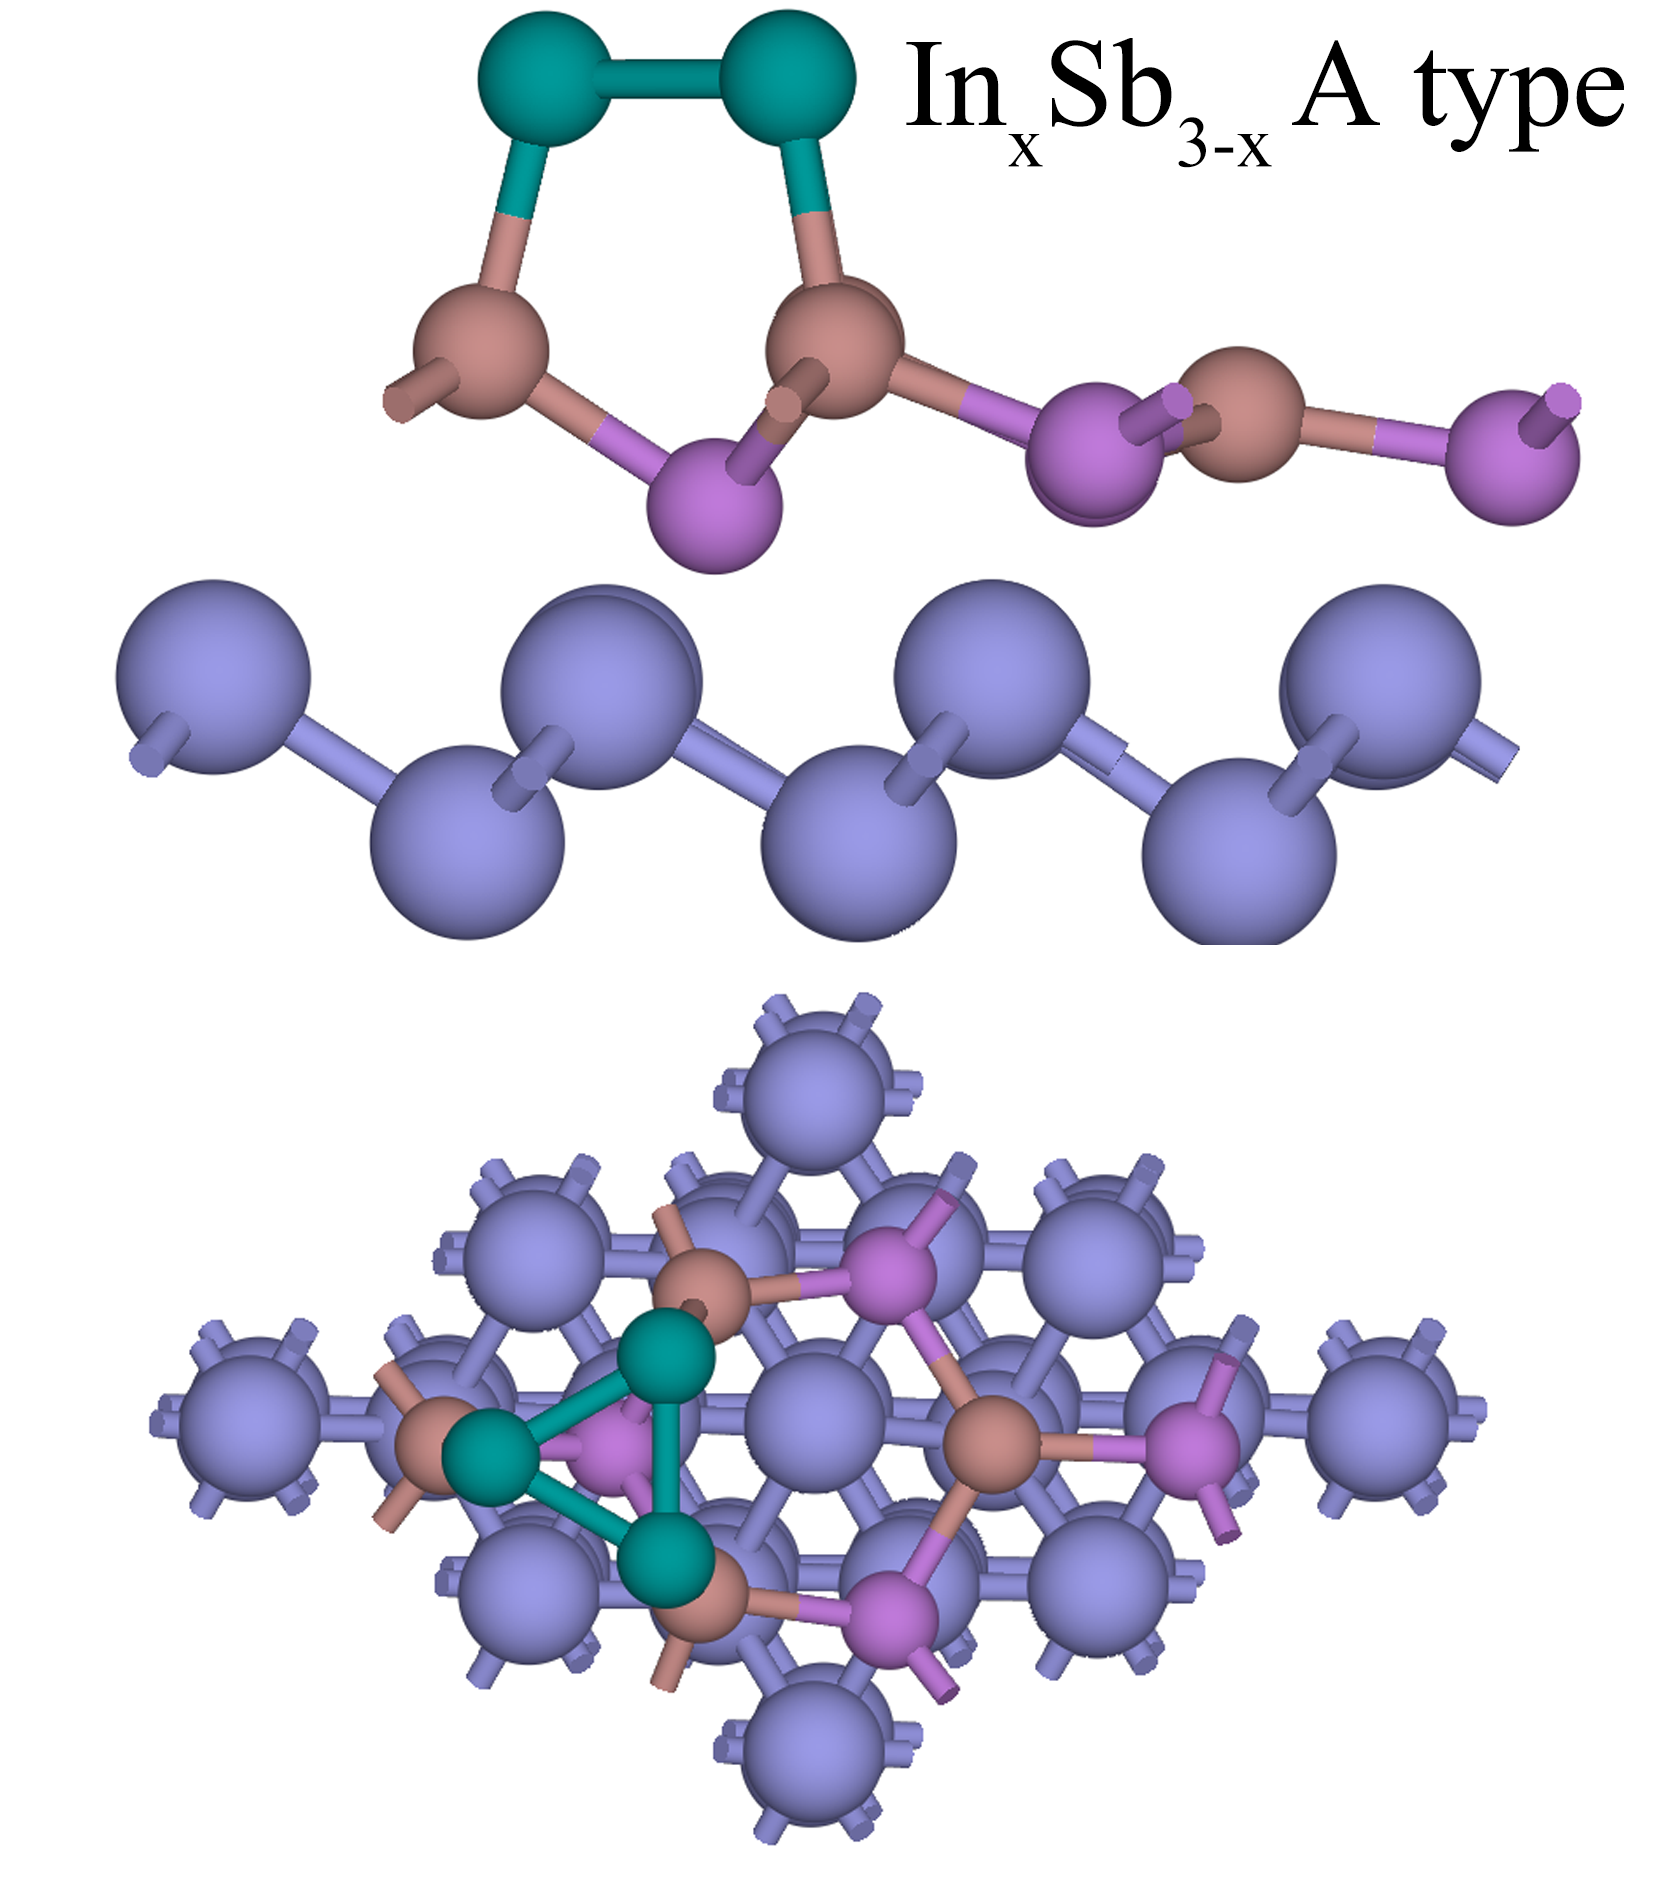
\includegraphics{pic/IS_structure_InxSb3-x_A.png}
    }
    \subfloat[]{
        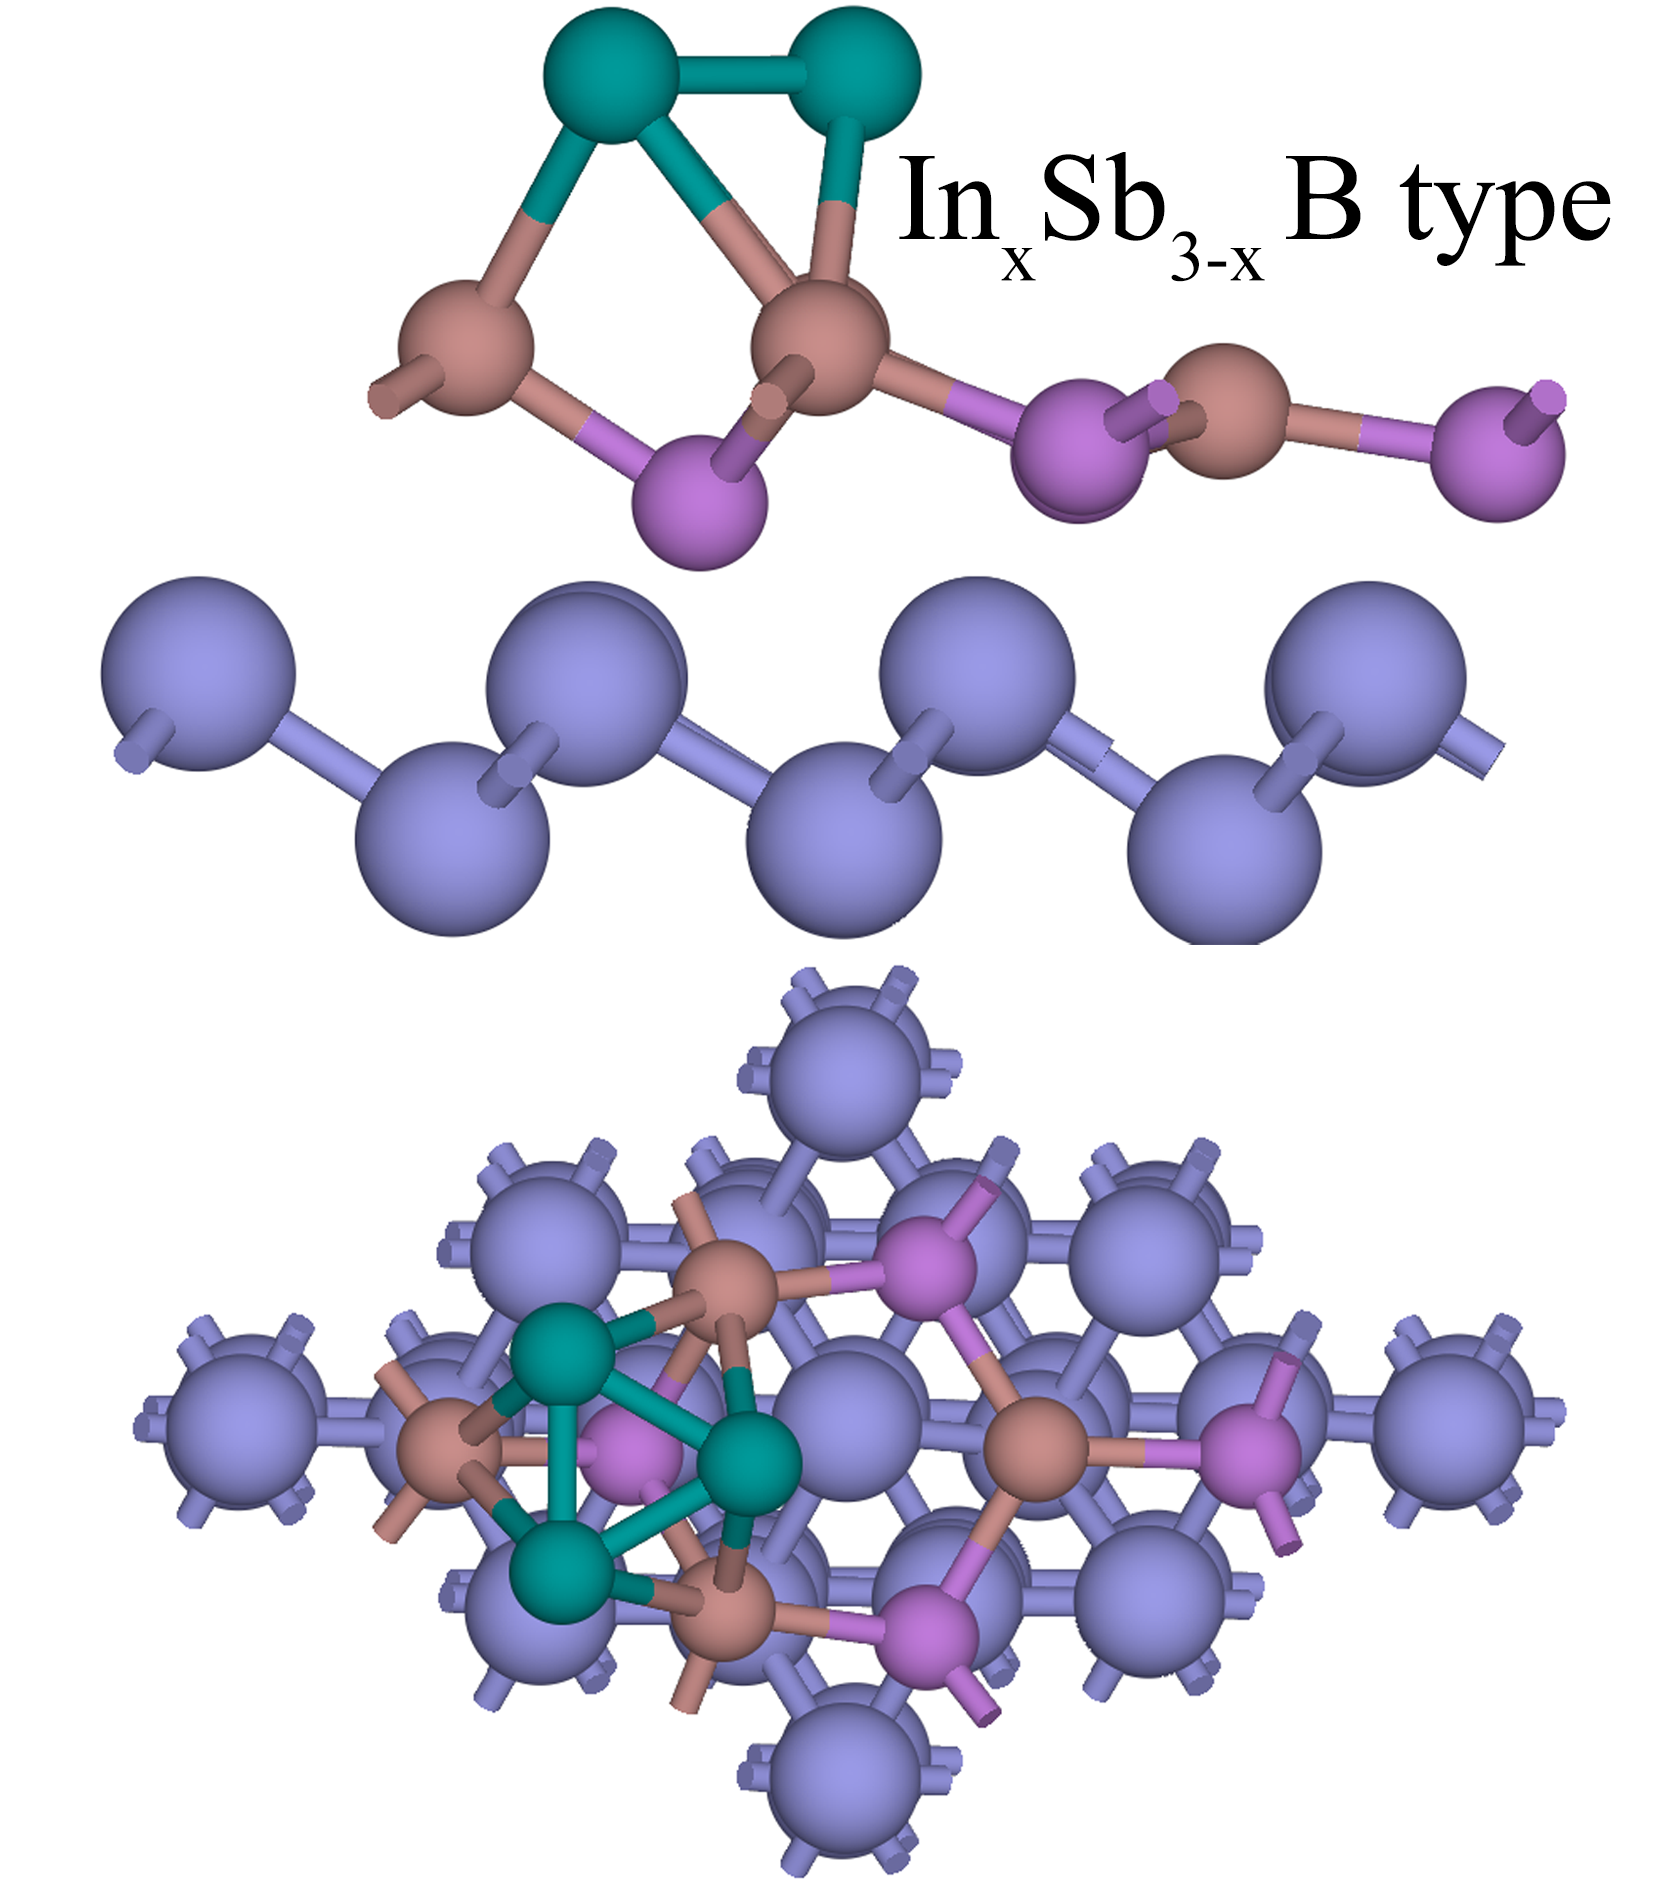
\includegraphics{pic/IS_structure_InxSb3-x_B.png}
    }
\end{figure}

\begin{figure}
    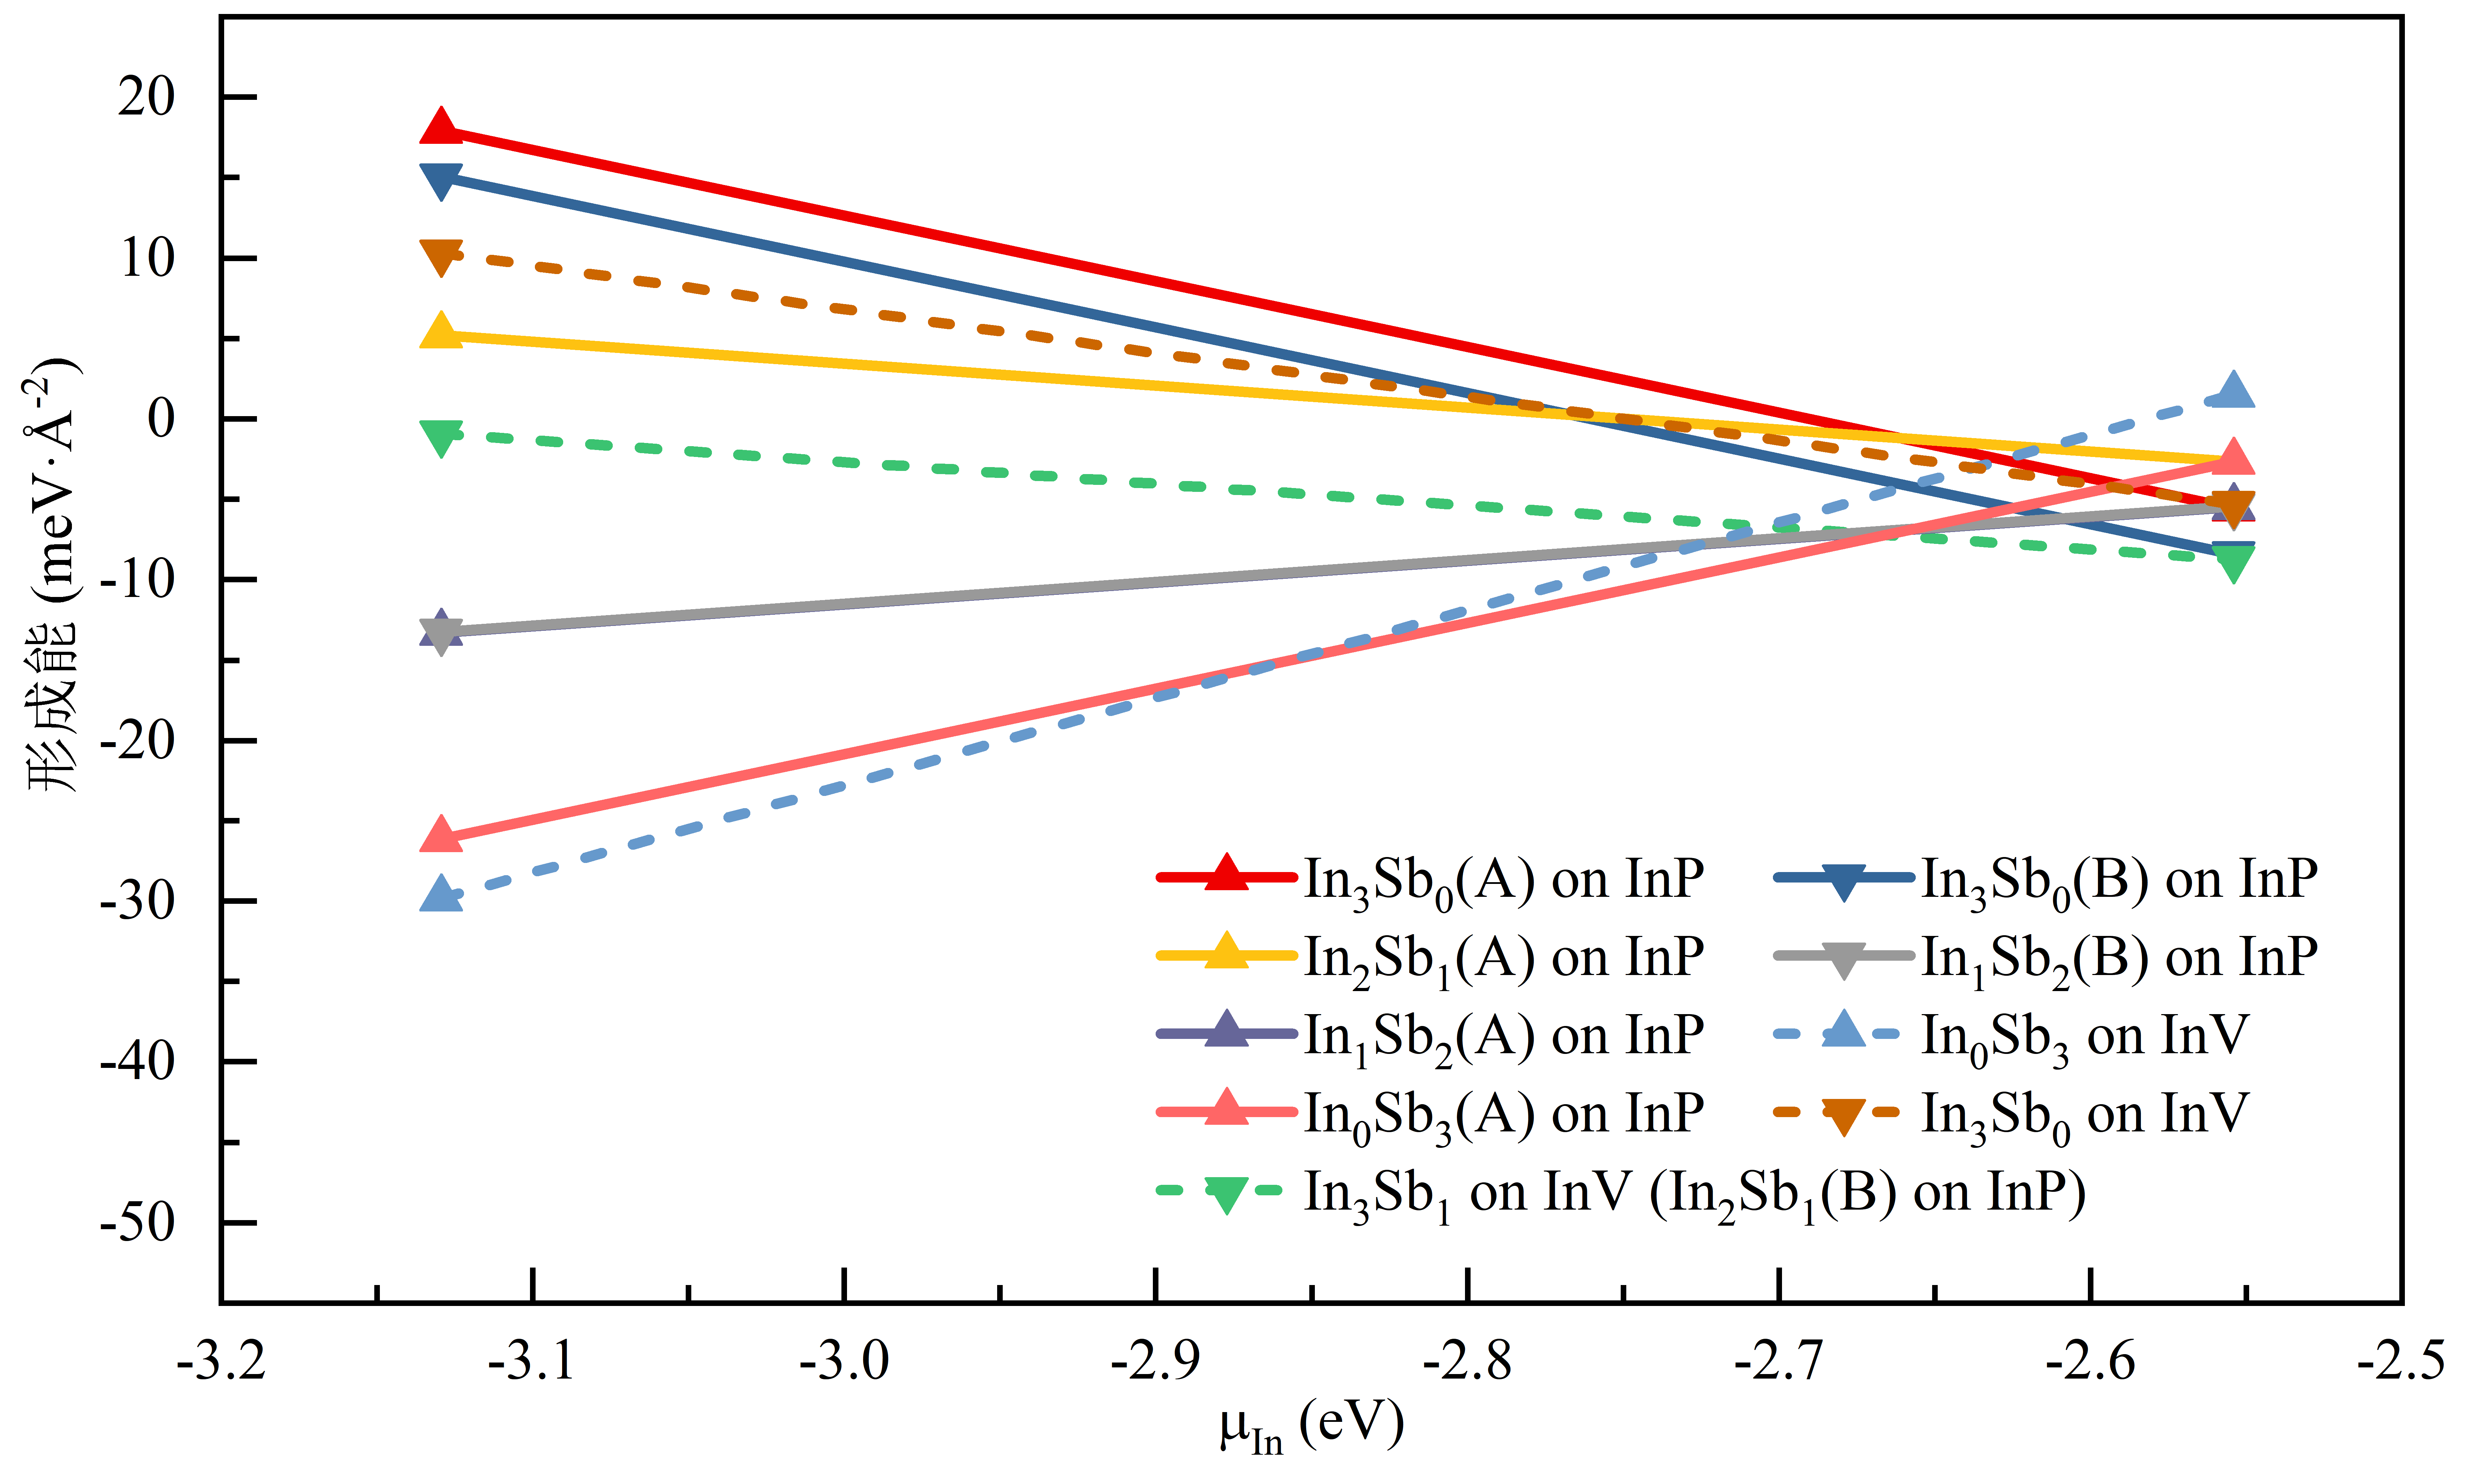
\includegraphics{pic/IS_DFT_2InSb_InxSbxT_All.png}
\end{figure}

\begin{figure}
    \subfloat[]{
        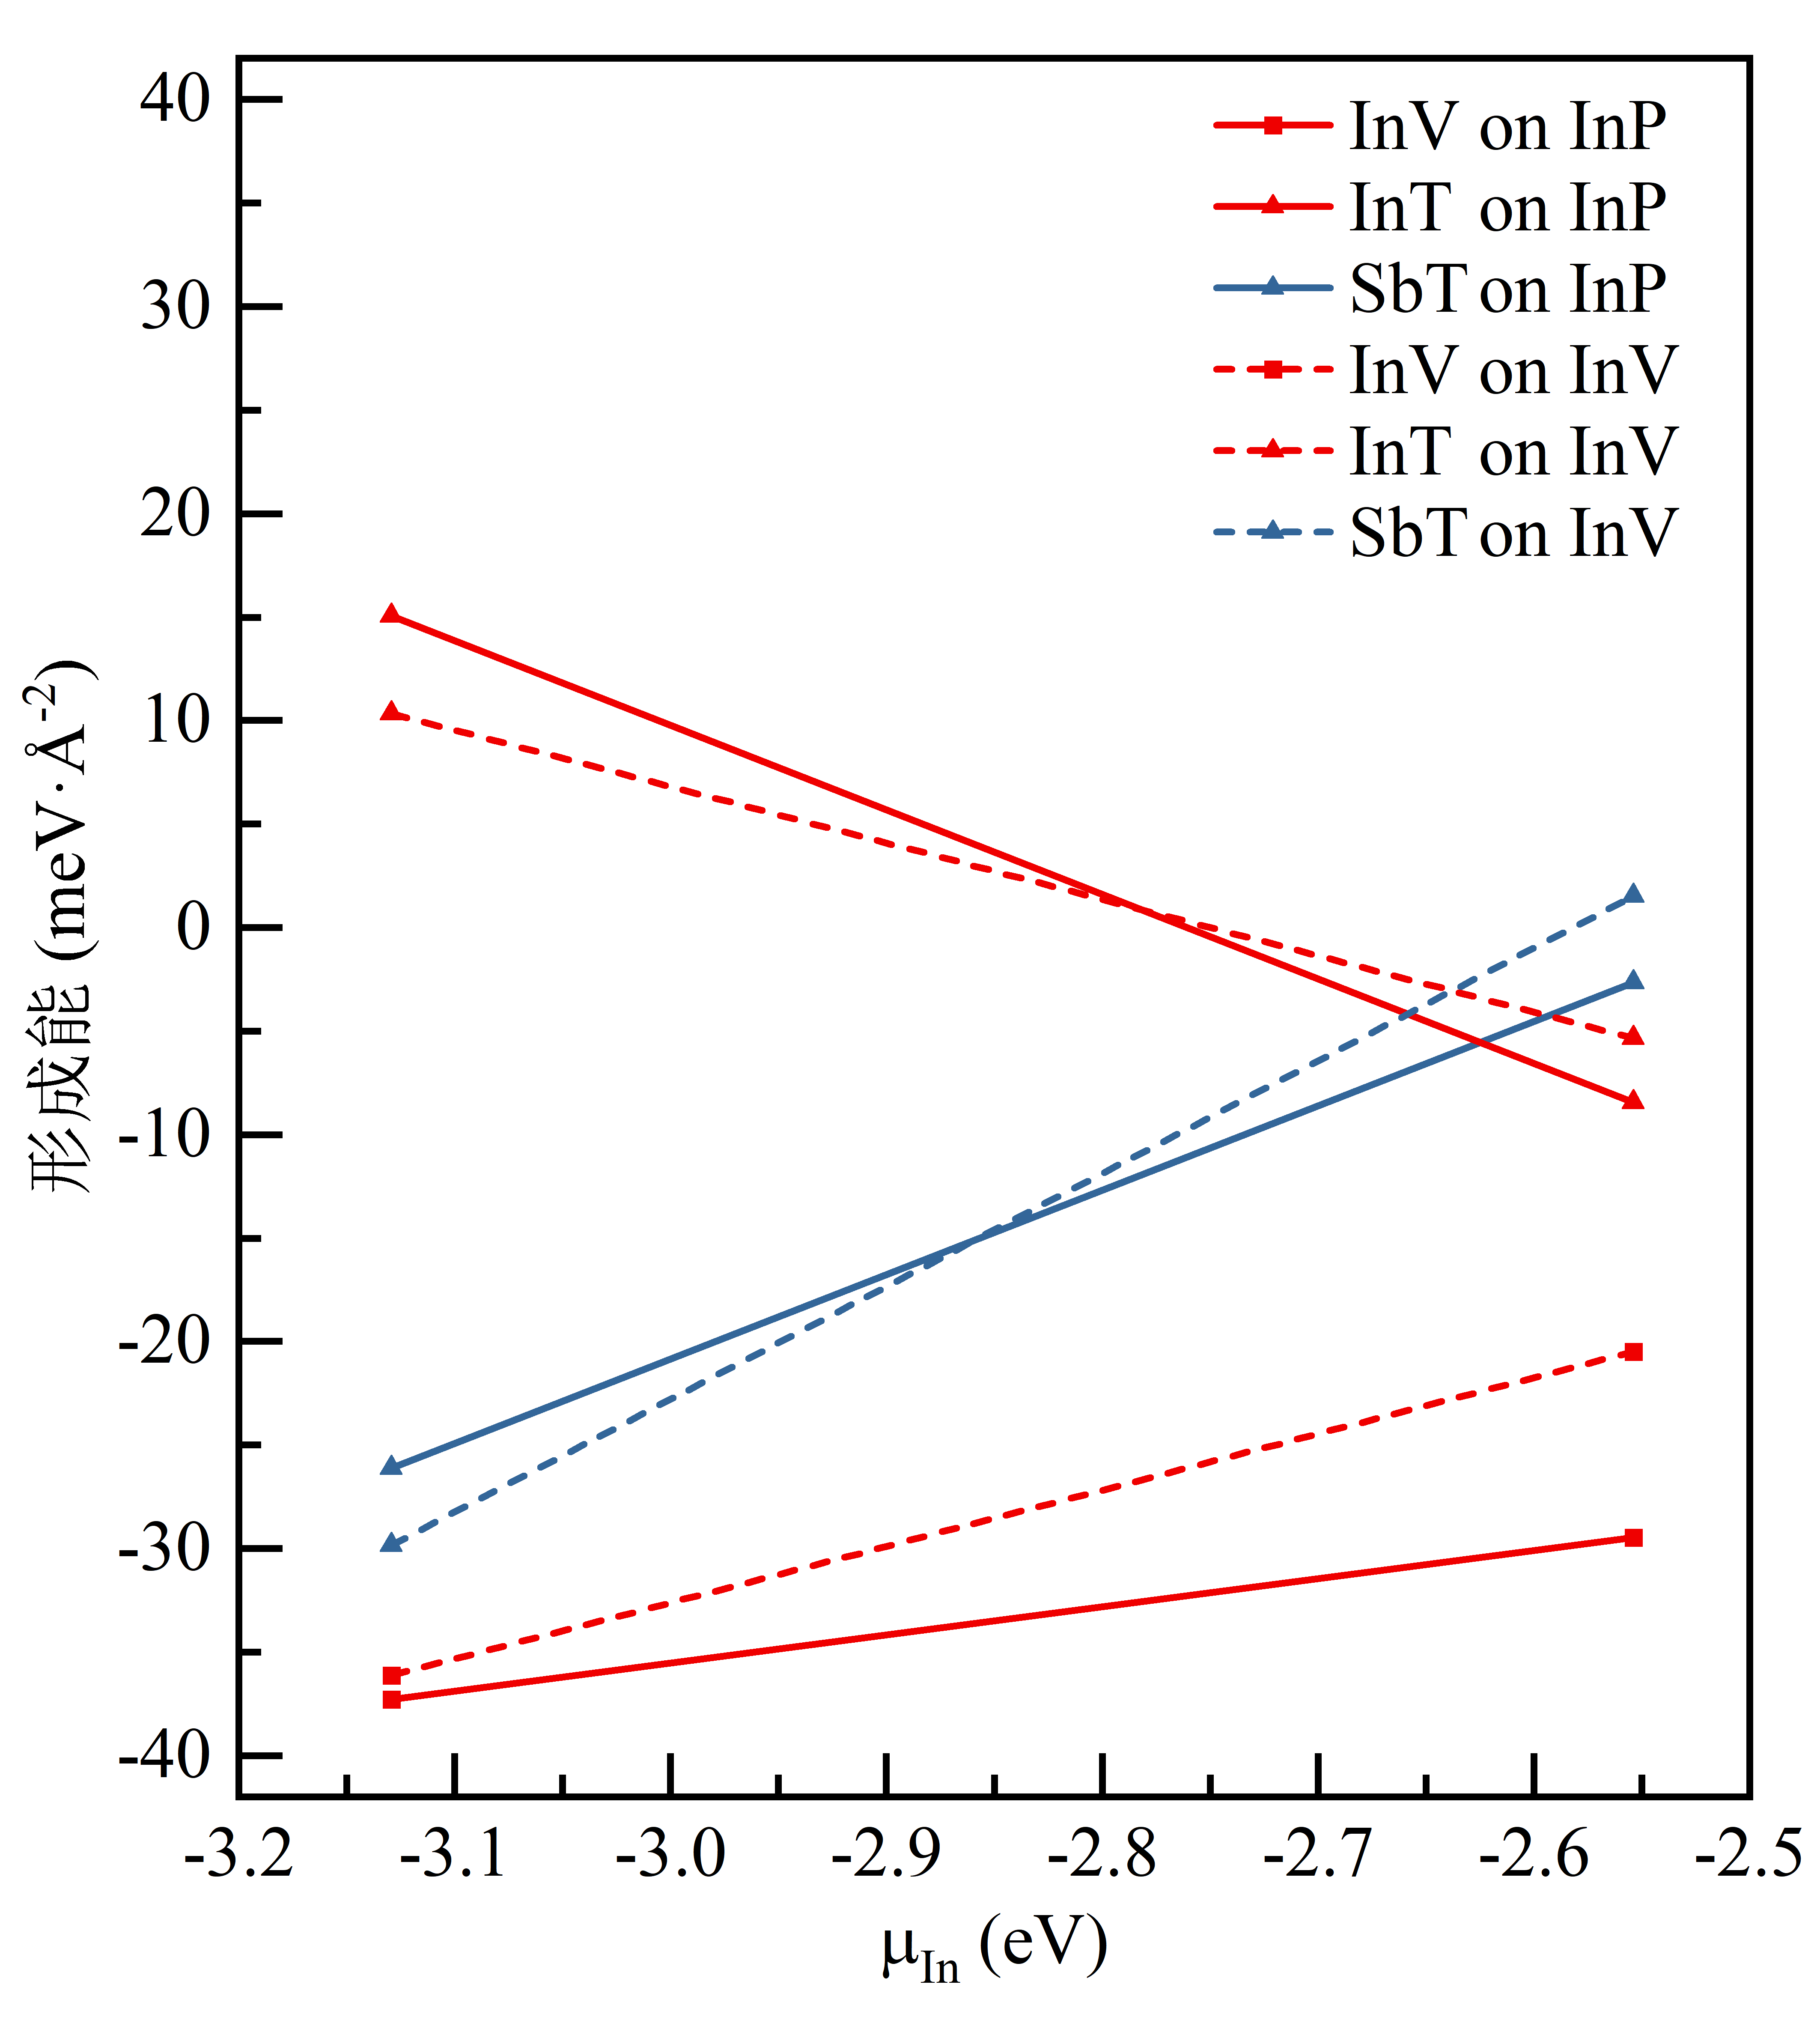
\includegraphics{pic/IS_DFT_2LInSb_SbT-InV-InT_InV-InP.png}
    }\hspace{-5mm}
    \begin{minipage}[b]{0.4\textwidth}
        \subfloat[]{
            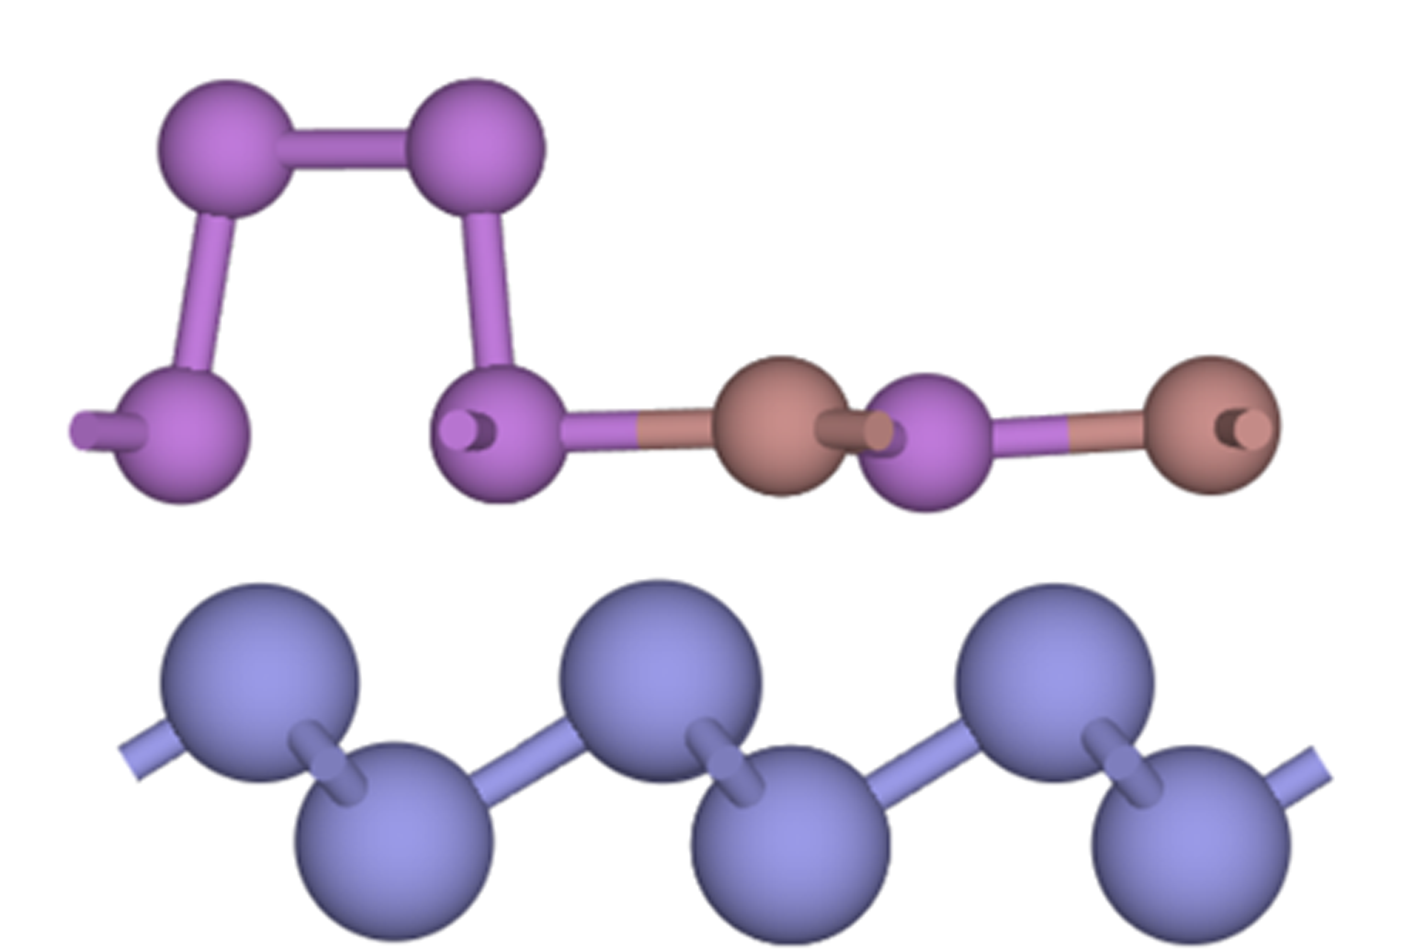
\includegraphics[width=0.9\textwidth]{pic/IS_structure_SbTonInV.png}
        }
        \newline
        \subfloat[]{
            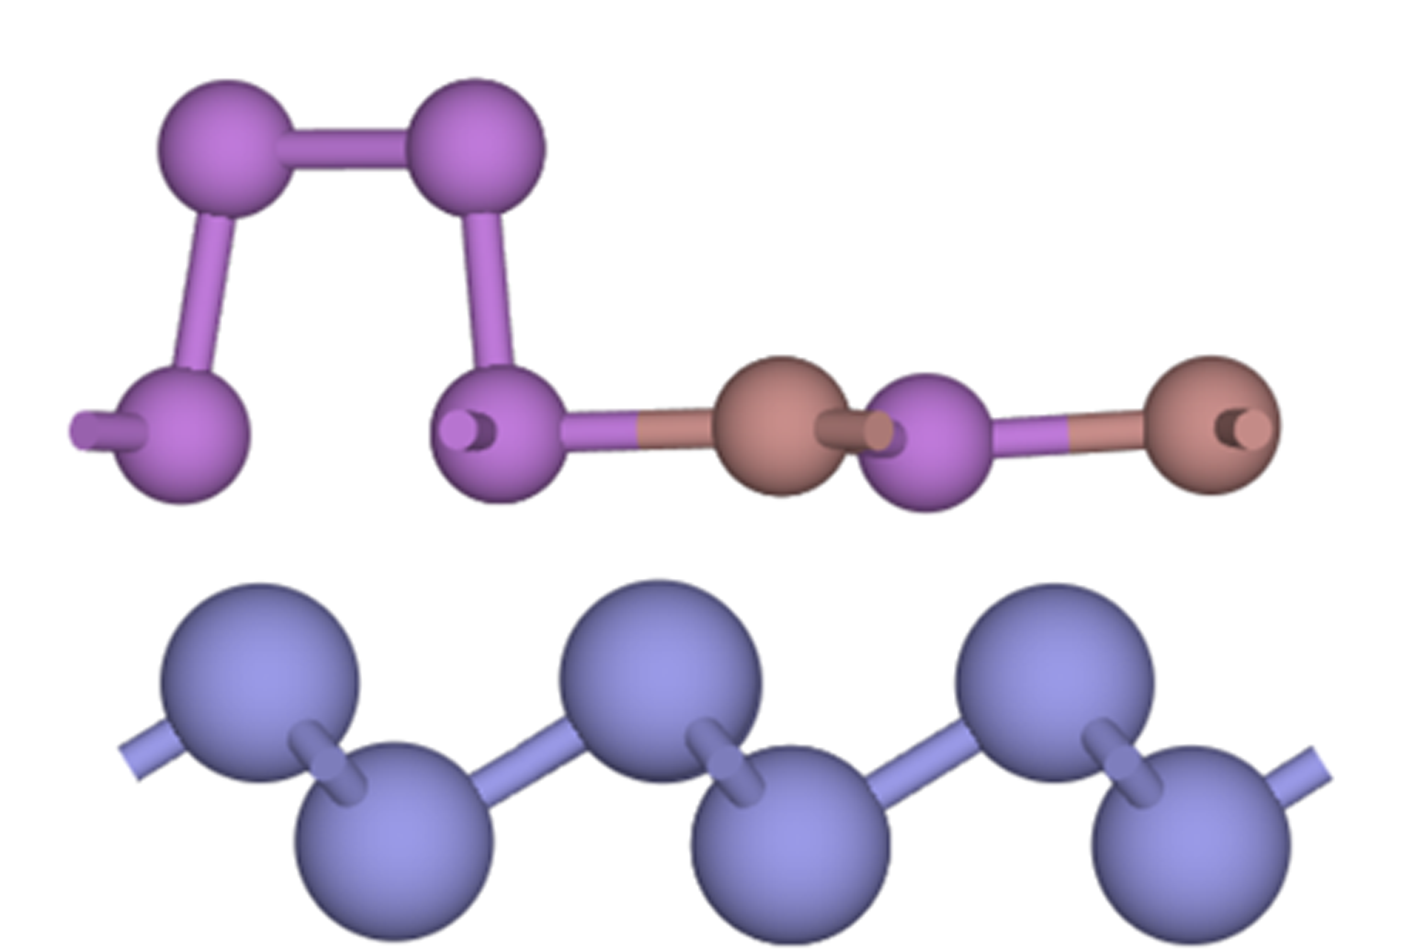
\includegraphics[width=0.9\textwidth]{pic/IS_structure_SbTonInV.png}
        }
    \end{minipage}
\end{figure}

\begin{figure}
    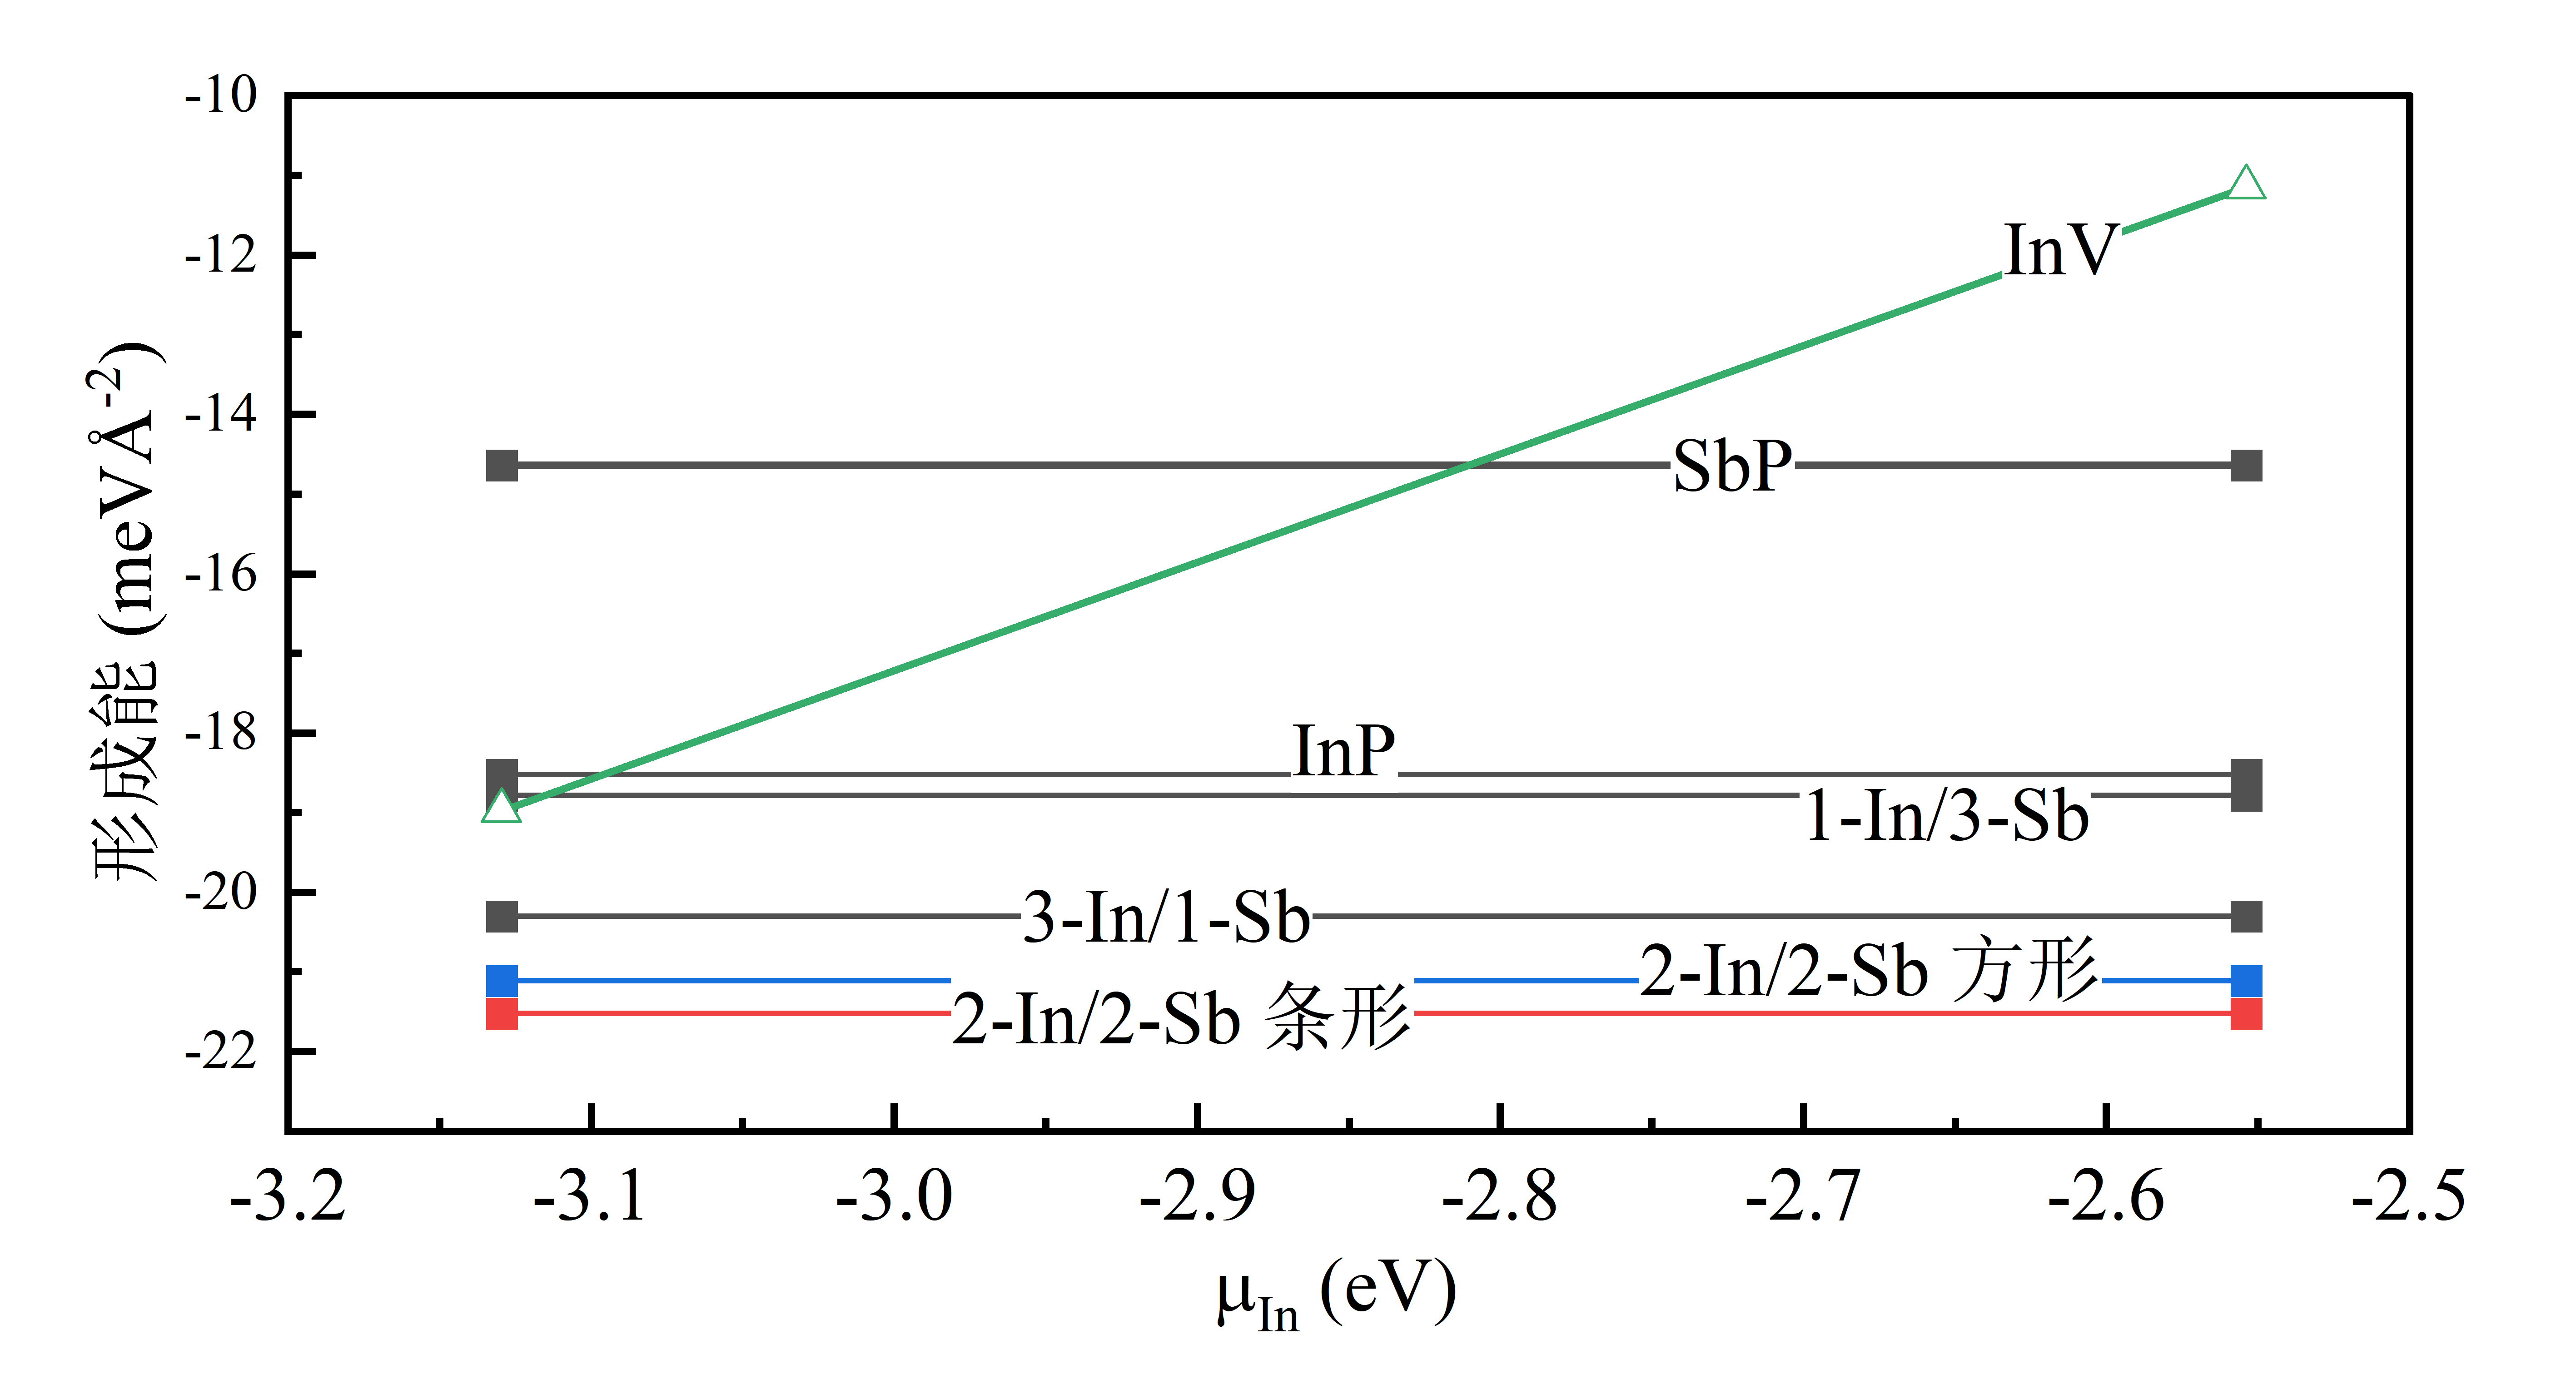
\includegraphics{pic/IS_DFT_1InSb_FlipVsInV.png}
\end{figure}

\begin{figure}
    \subfloat[]{
        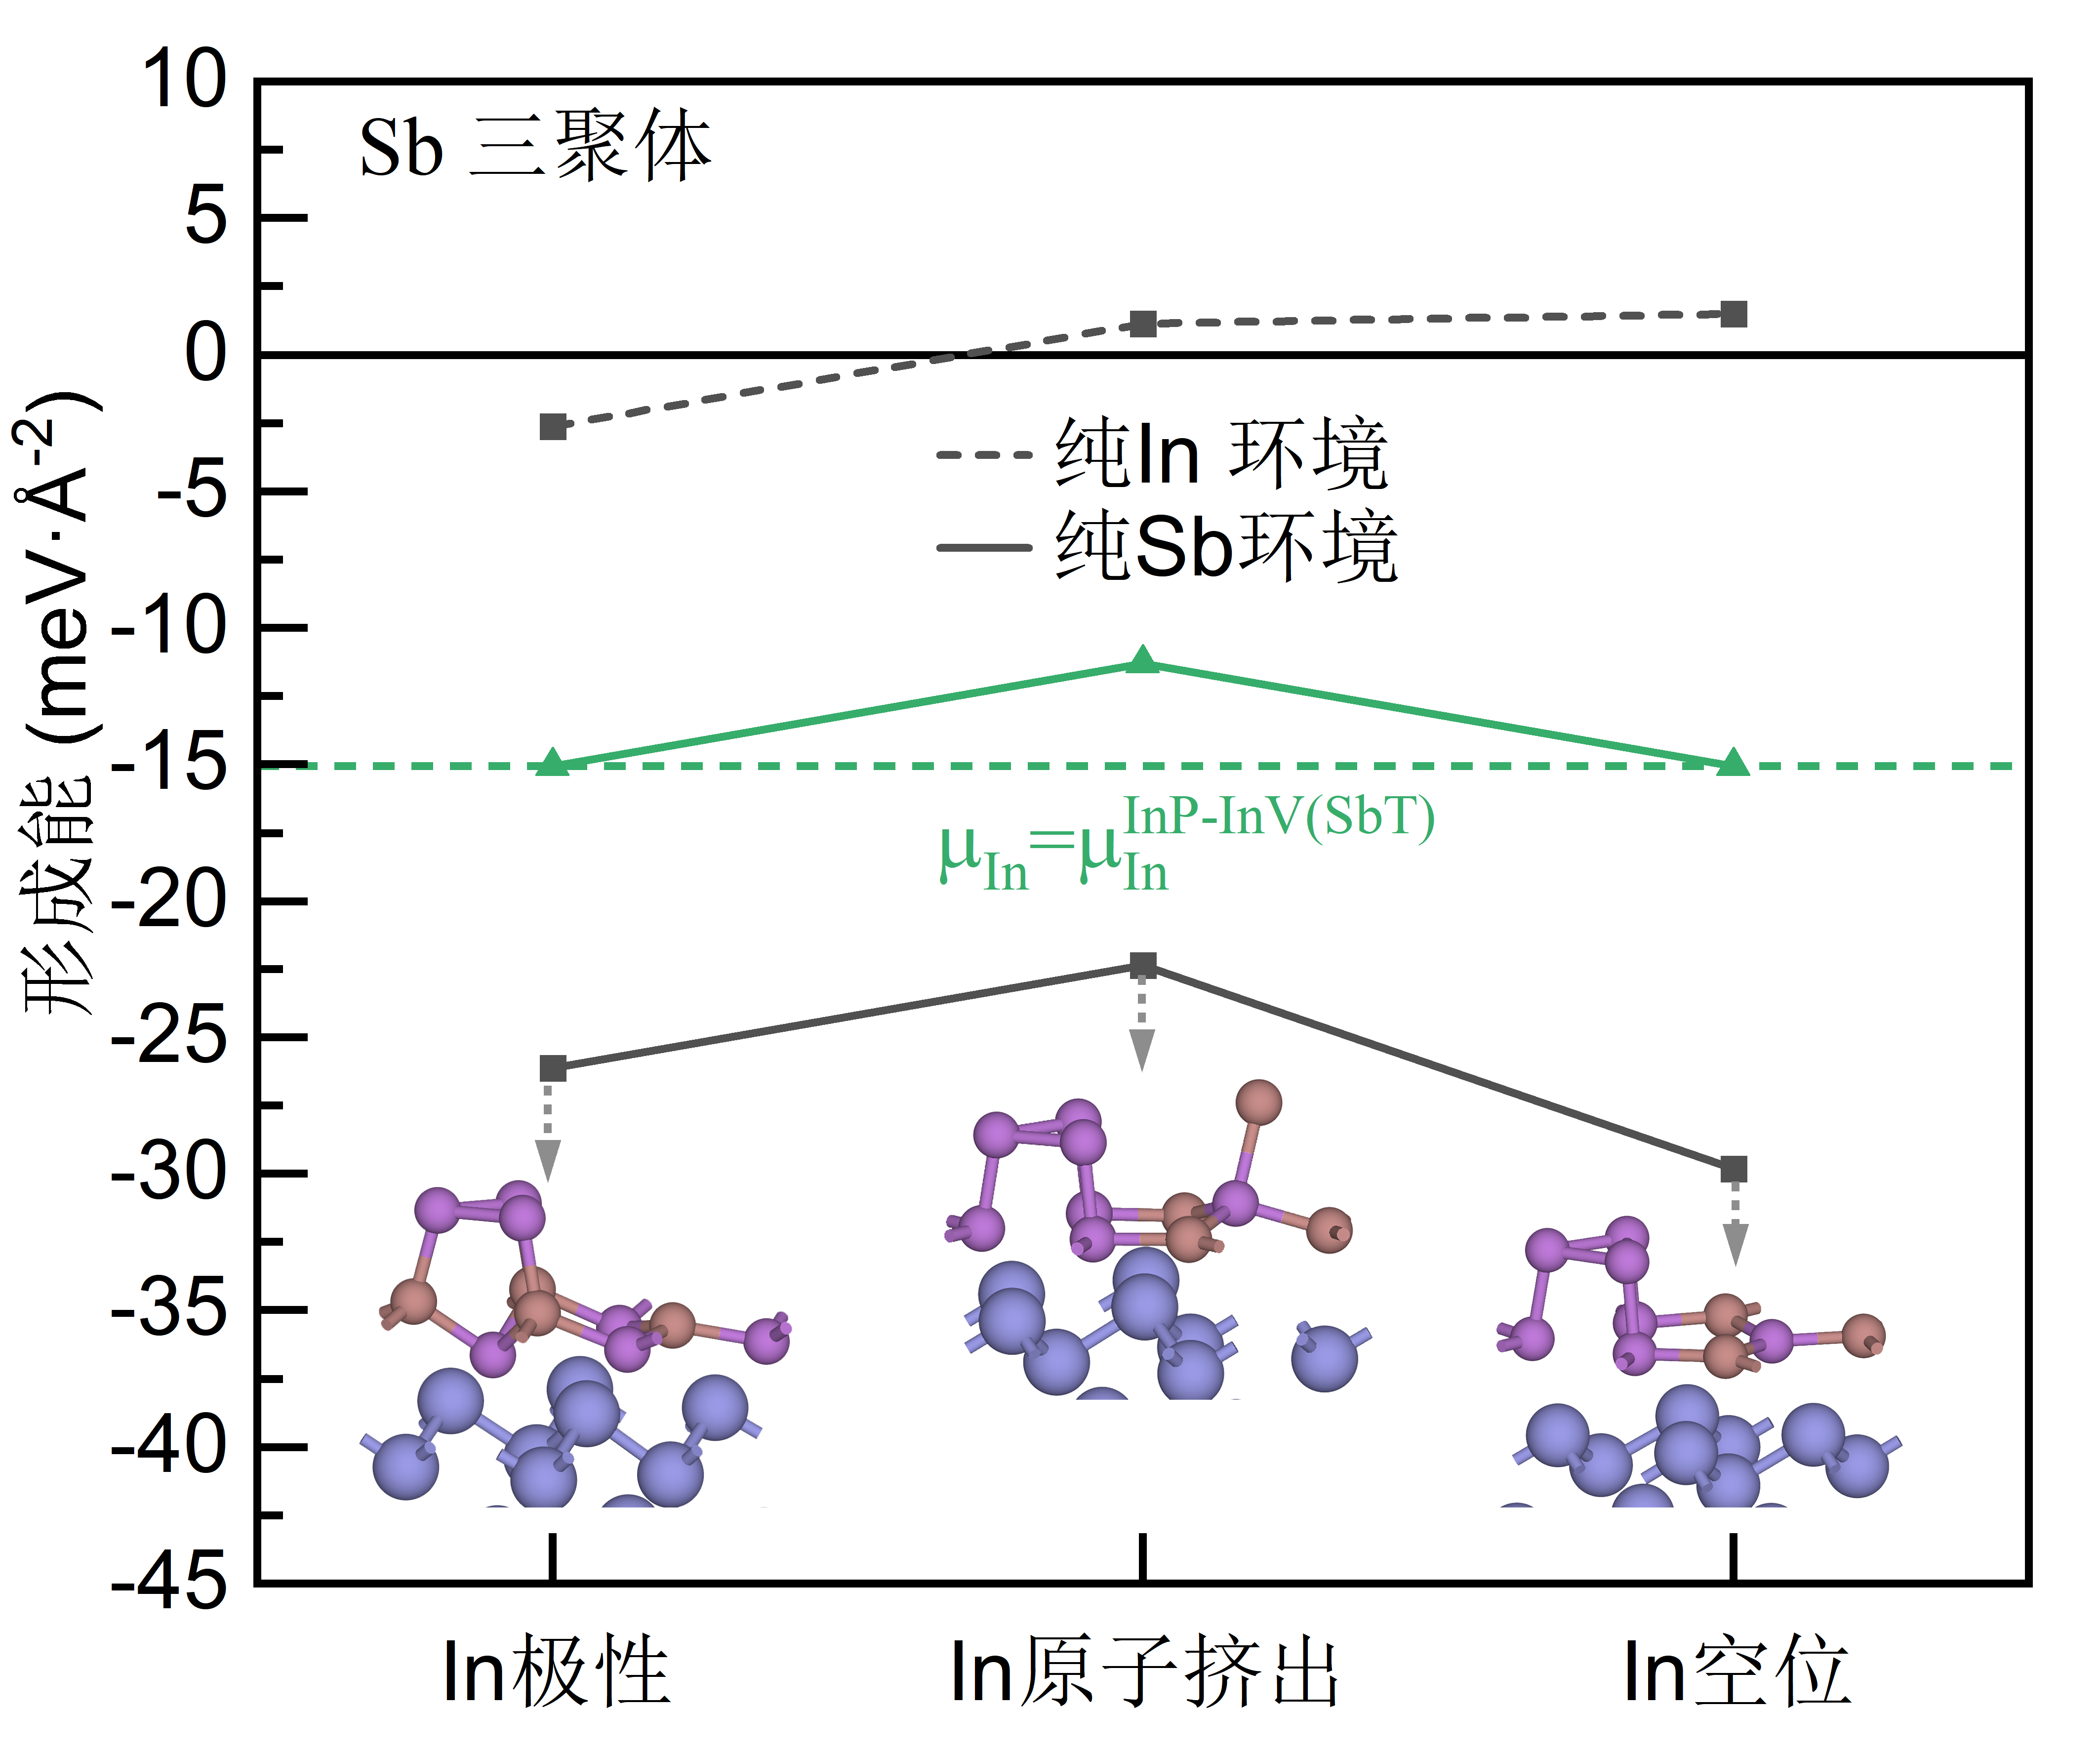
\includegraphics{pic/IS_DFT_2InSb_InPtoInV.png}
    }
    \subfloat[]{
        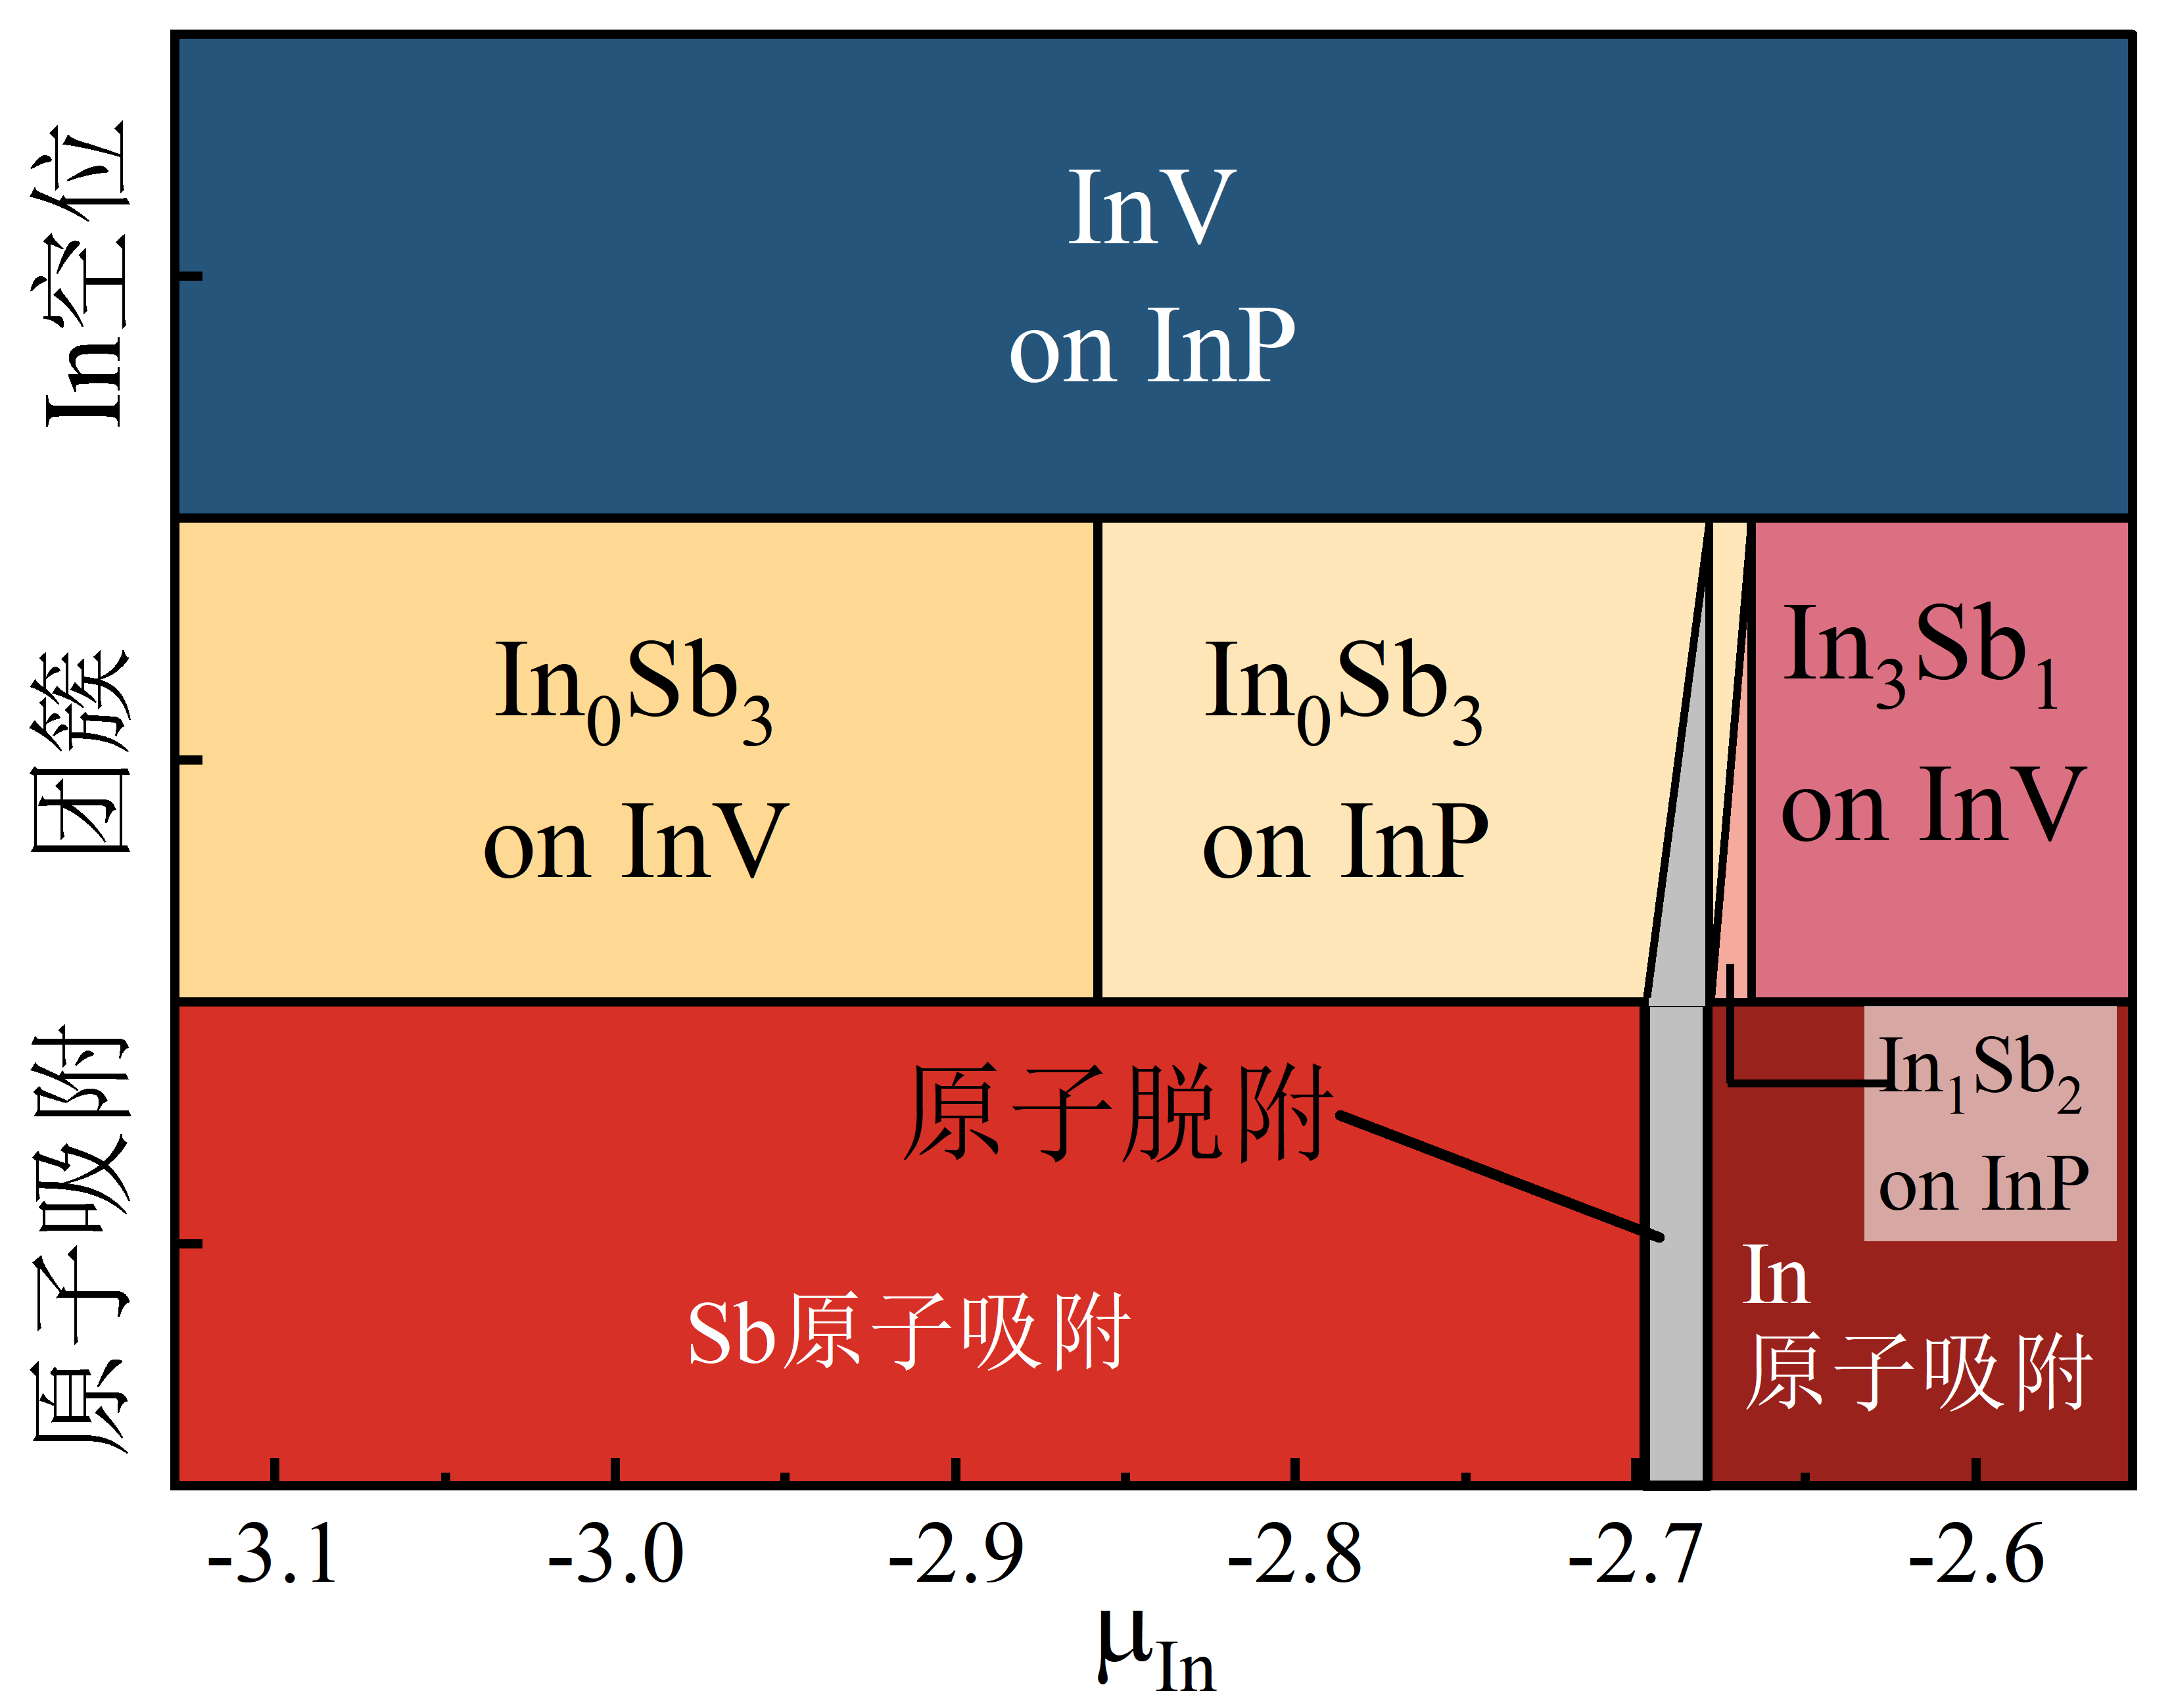
\includegraphics{pic/IS_DFT_stagePhase.png}
    }
\end{figure}
\subsection{双层锑化铟的极性演化}
\begin{figure}
    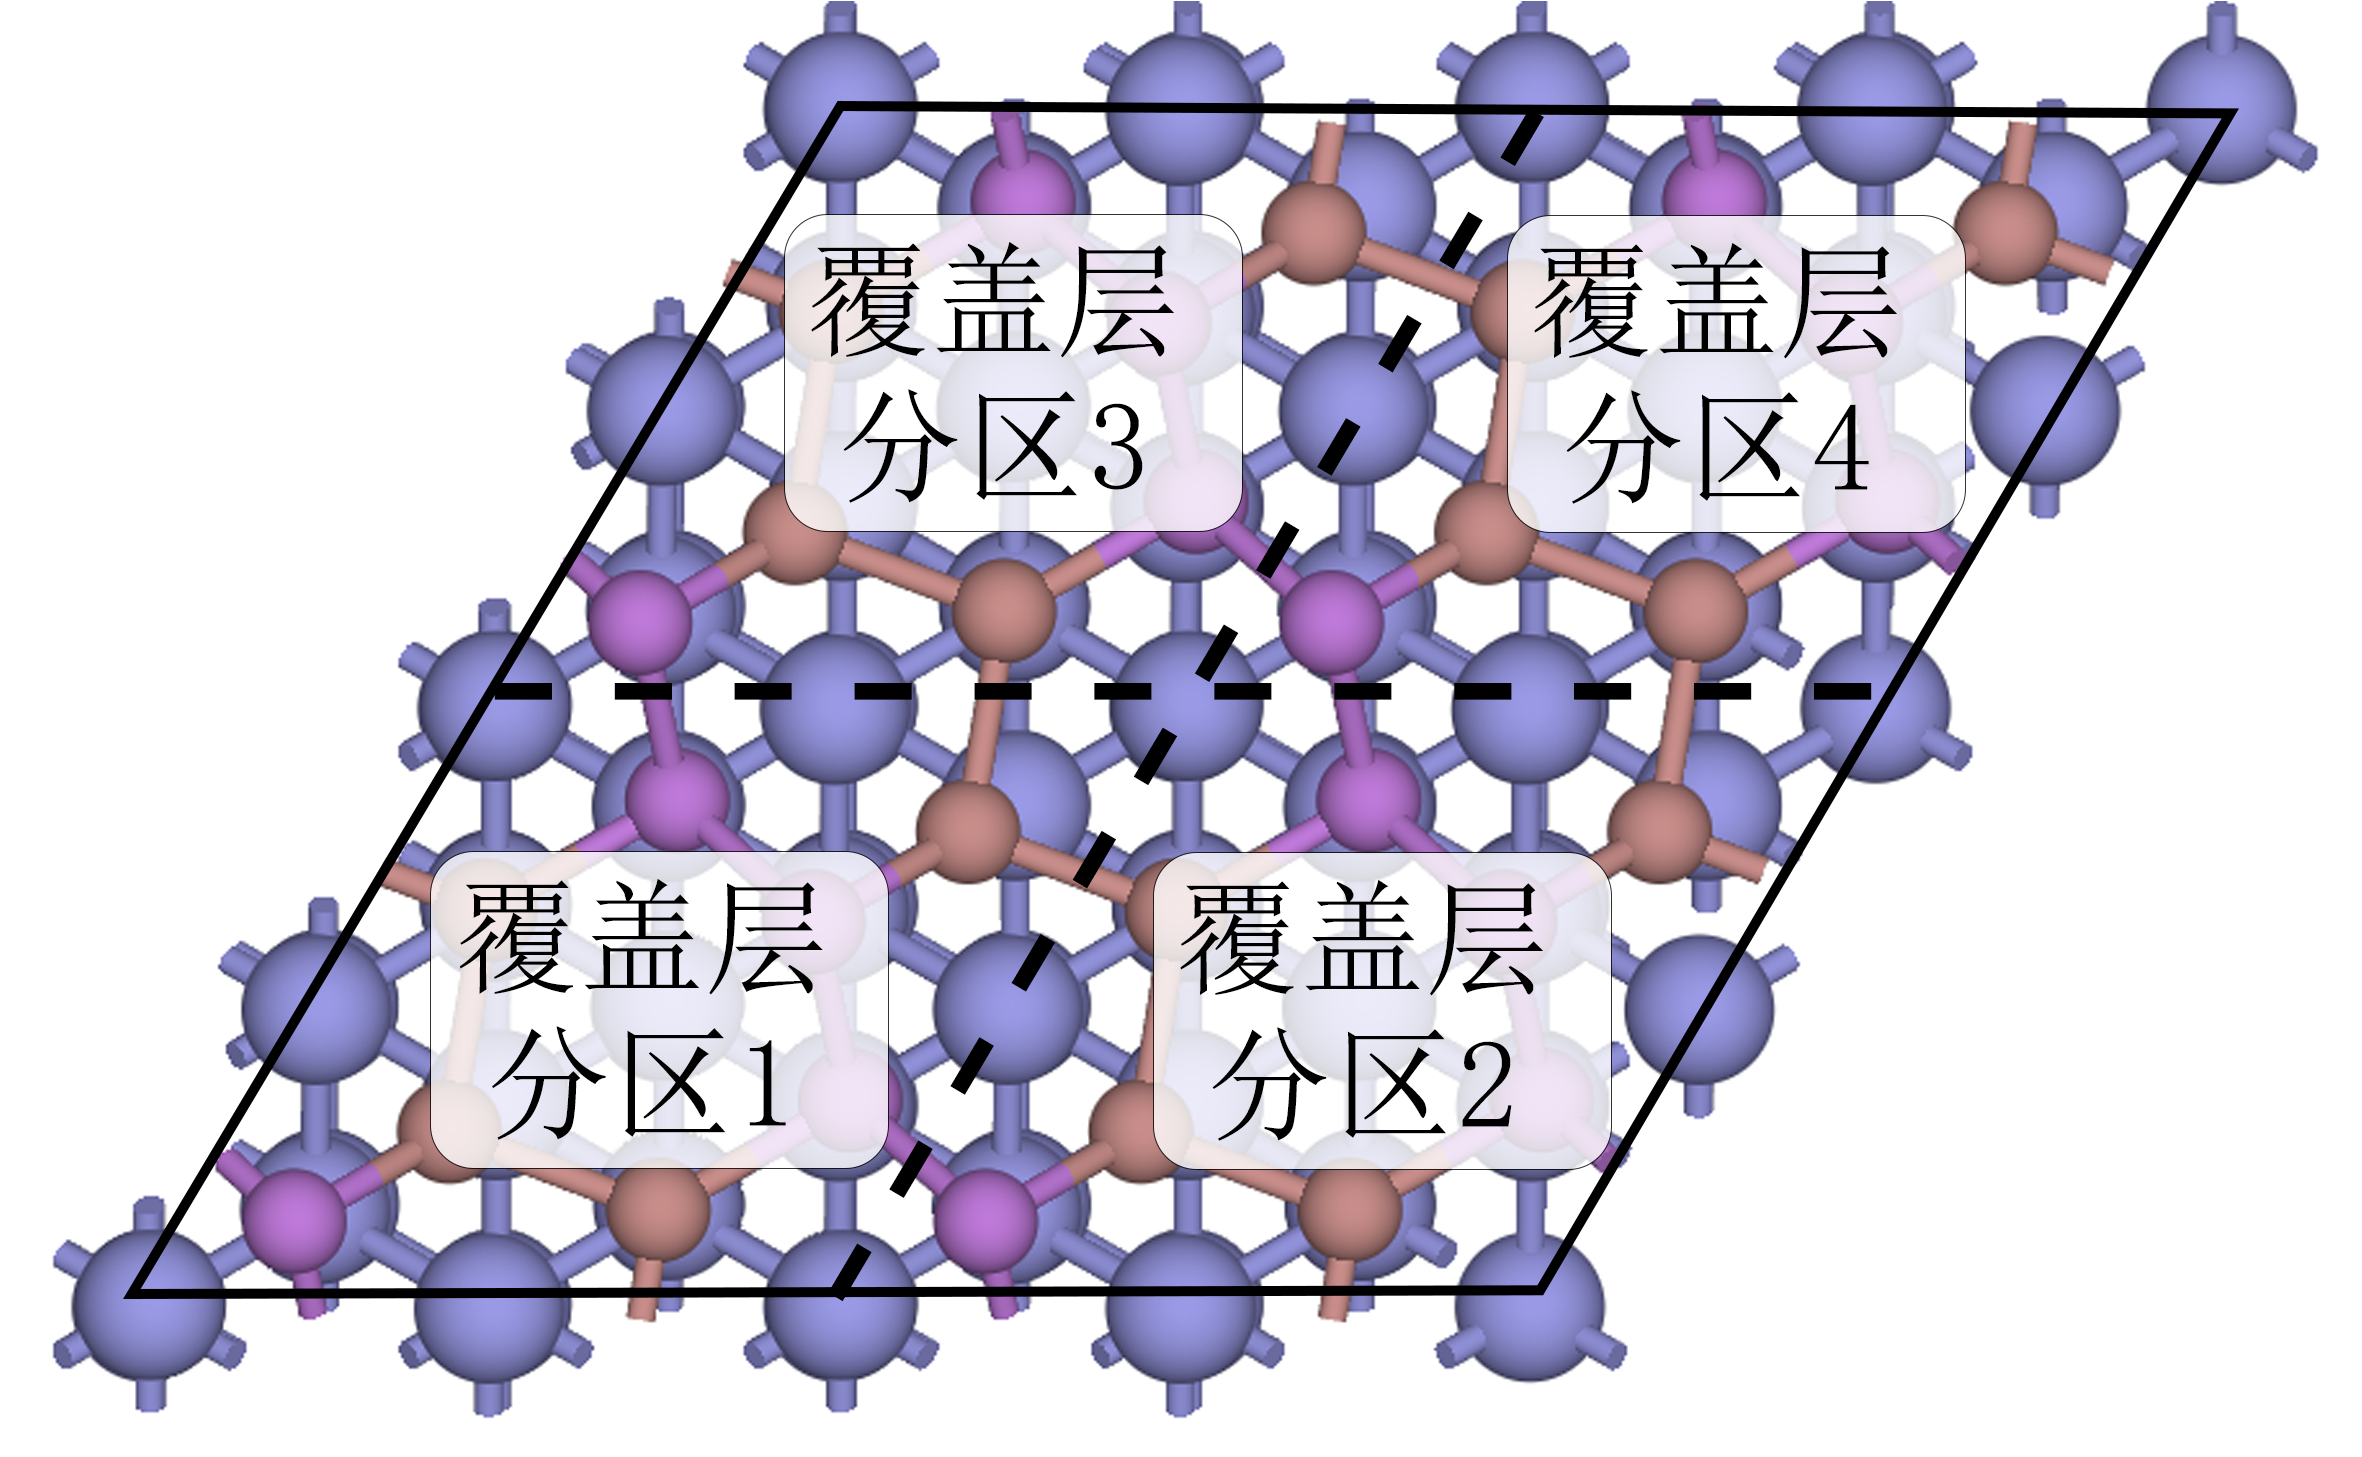
\includegraphics{pic/IS_diagram_2Linsb_partial.png}
\end{figure}

\begin{figure}
    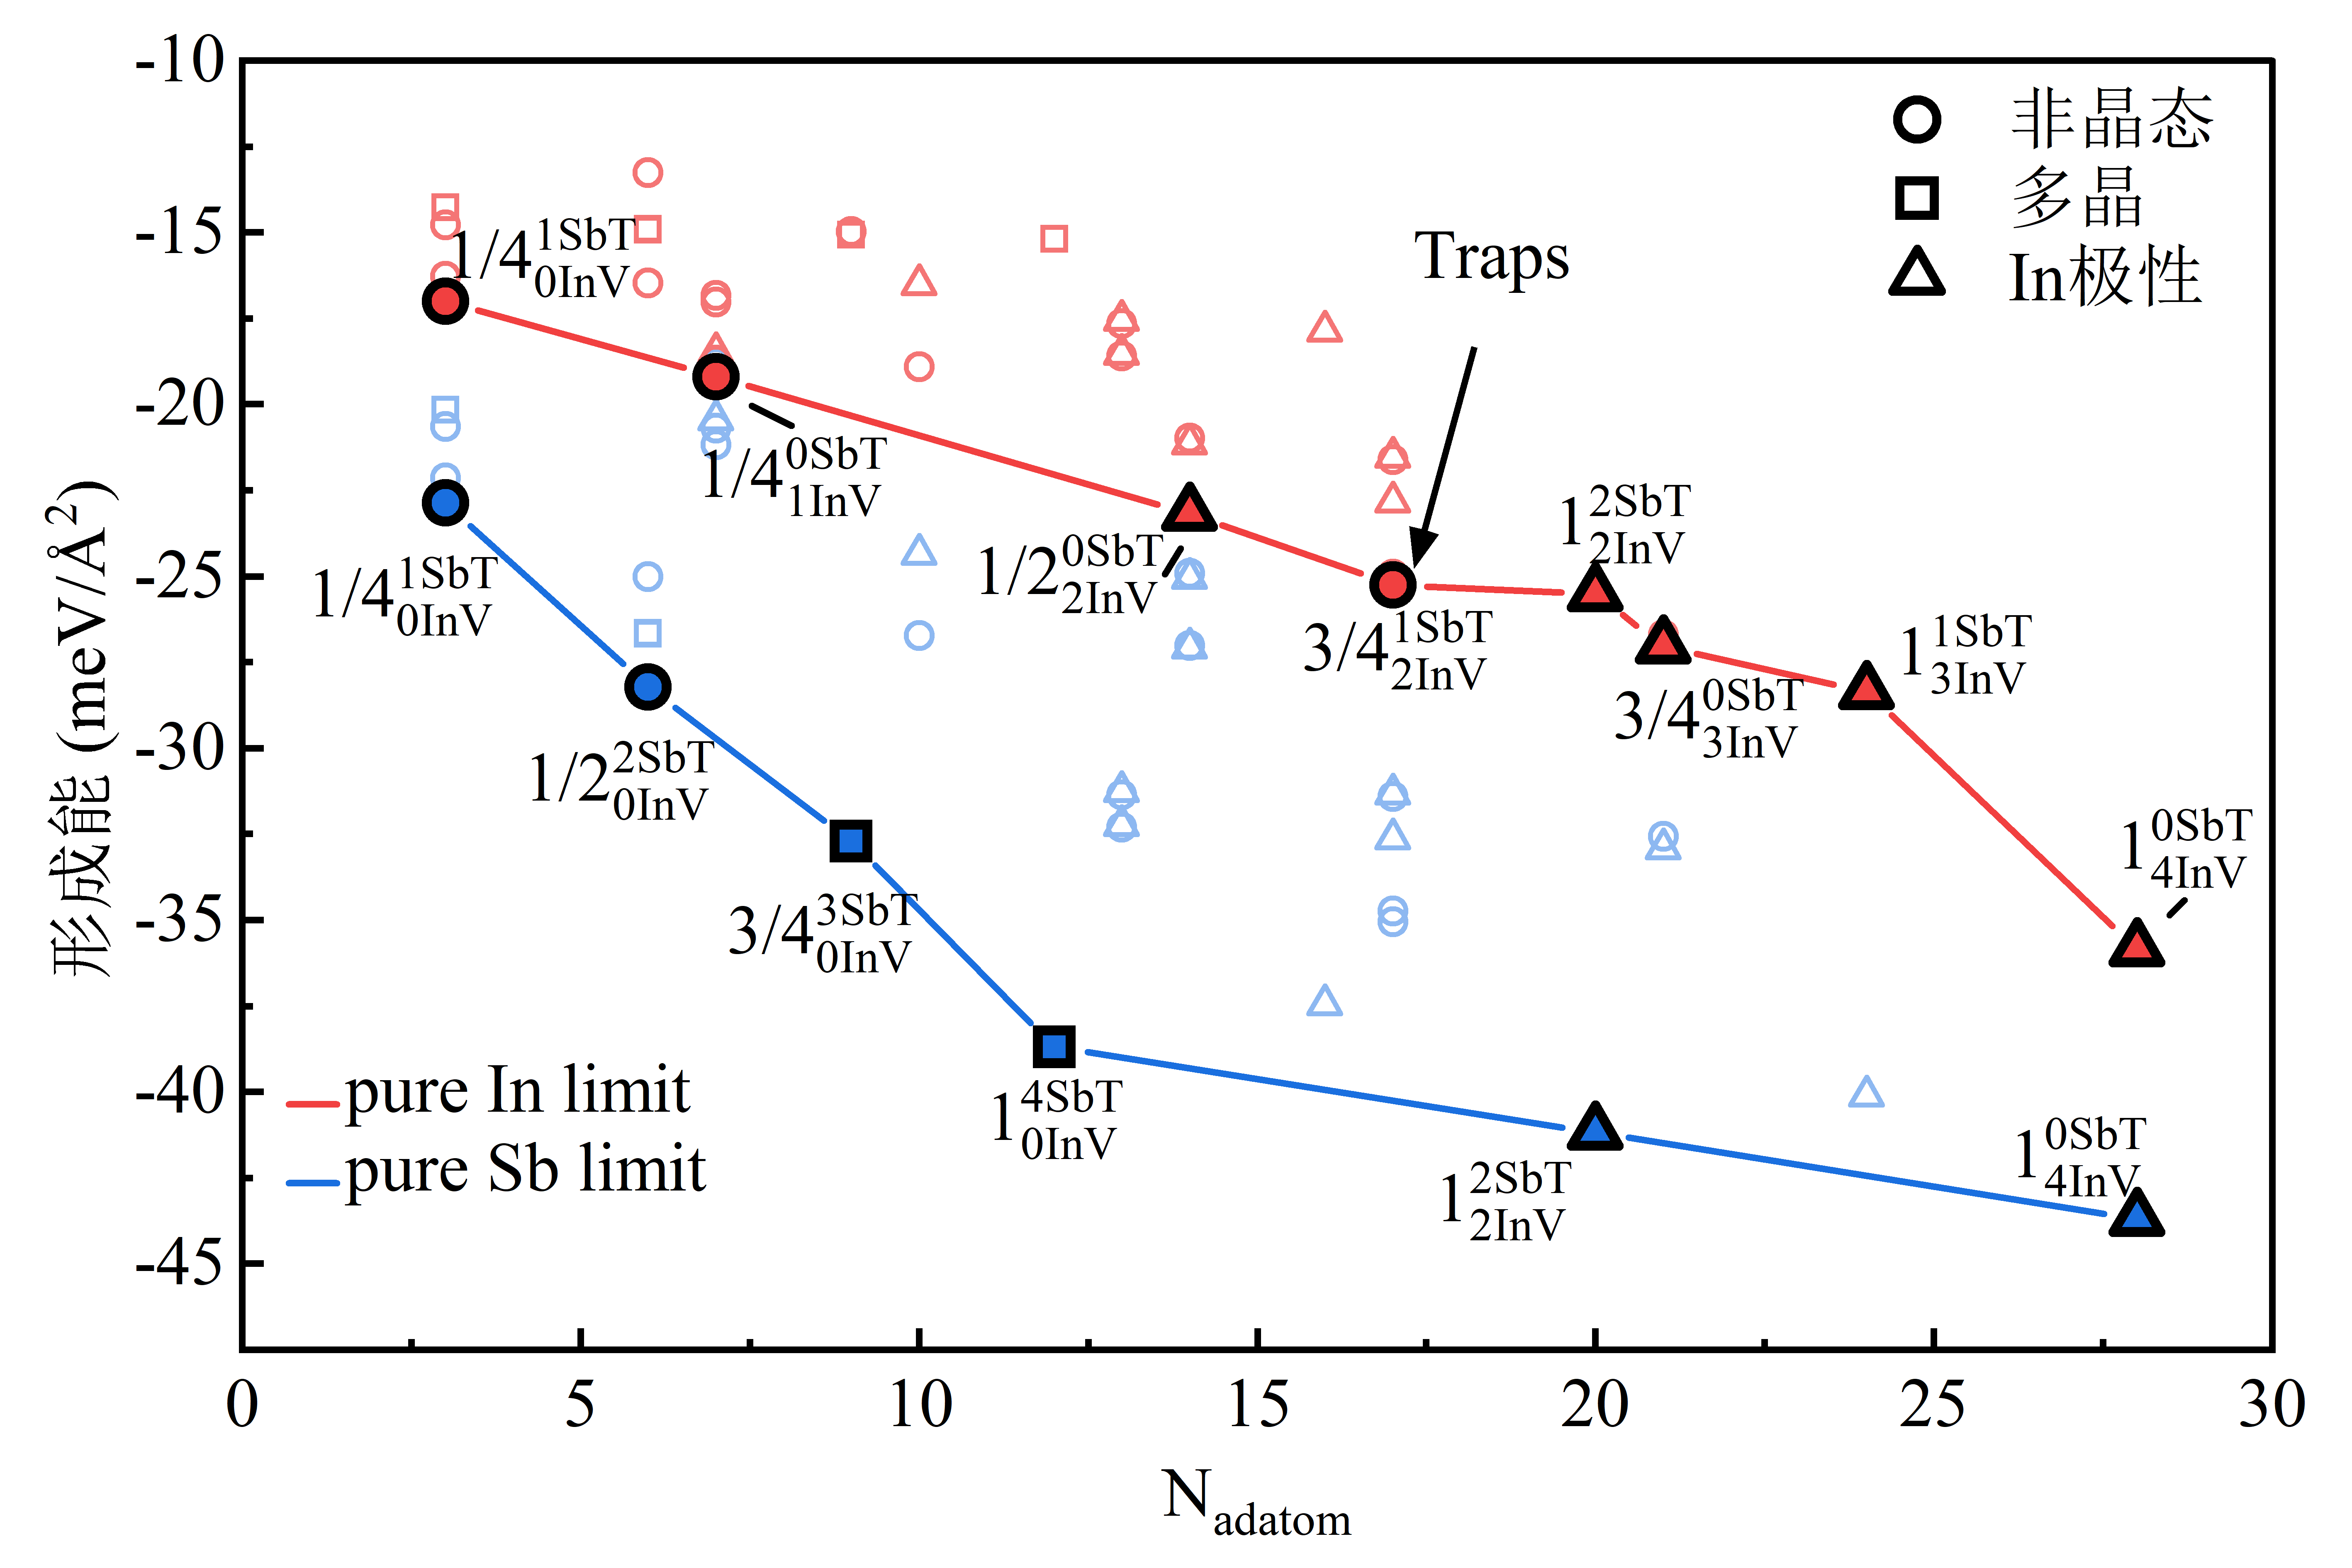
\includegraphics{pic/IS_DFT_2LInSb_partEnergy.png}
\end{figure}

\begin{figure}
    \subfloat[]{
        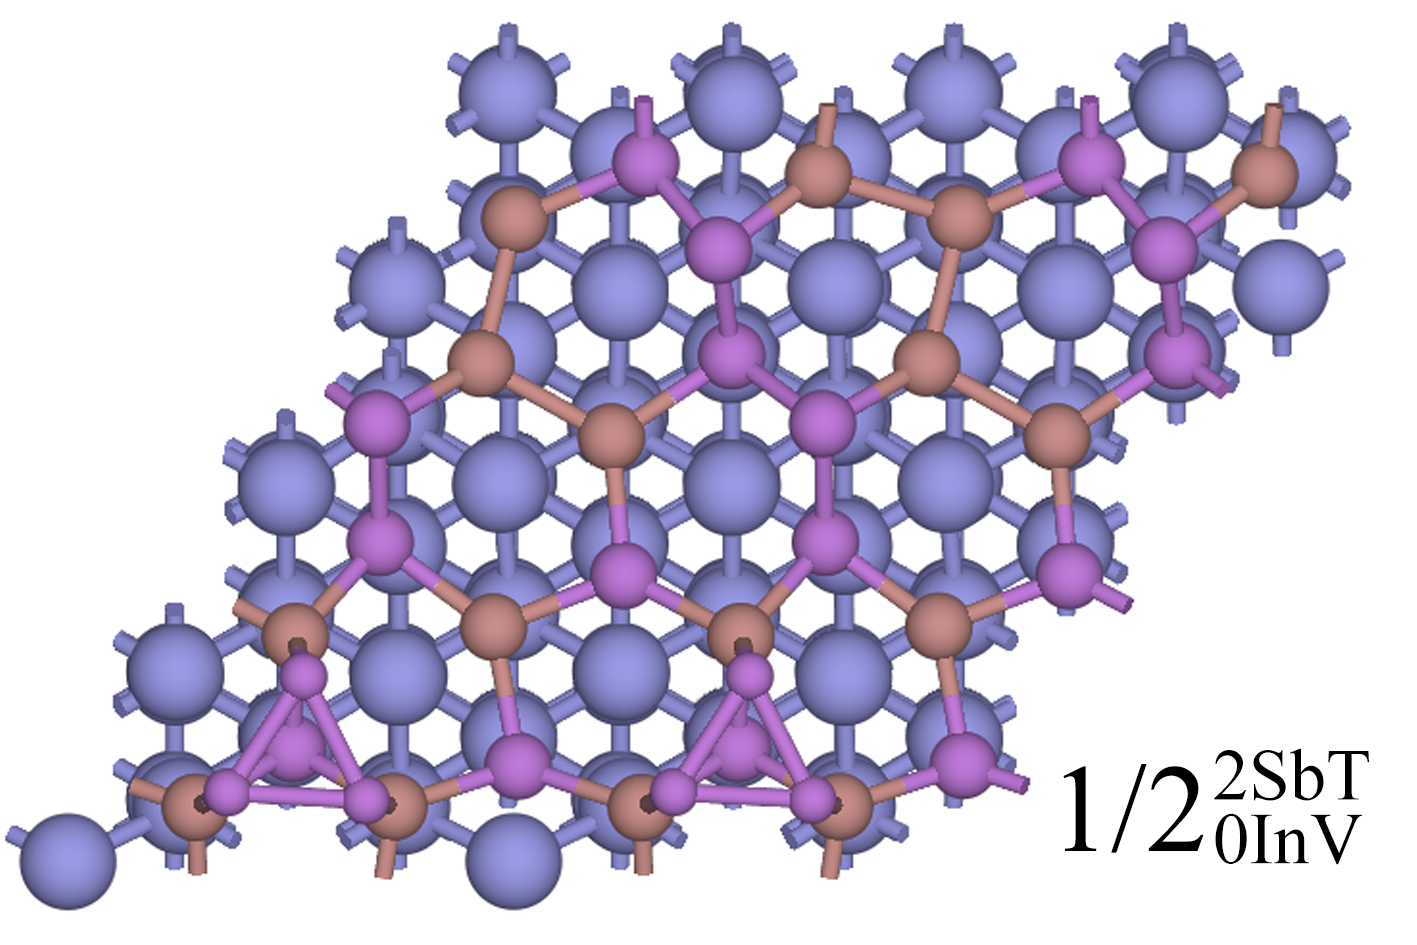
\includegraphics{pic/IS_structure_partical_1-2_0-2.png}
    }
    \subfloat[]{
        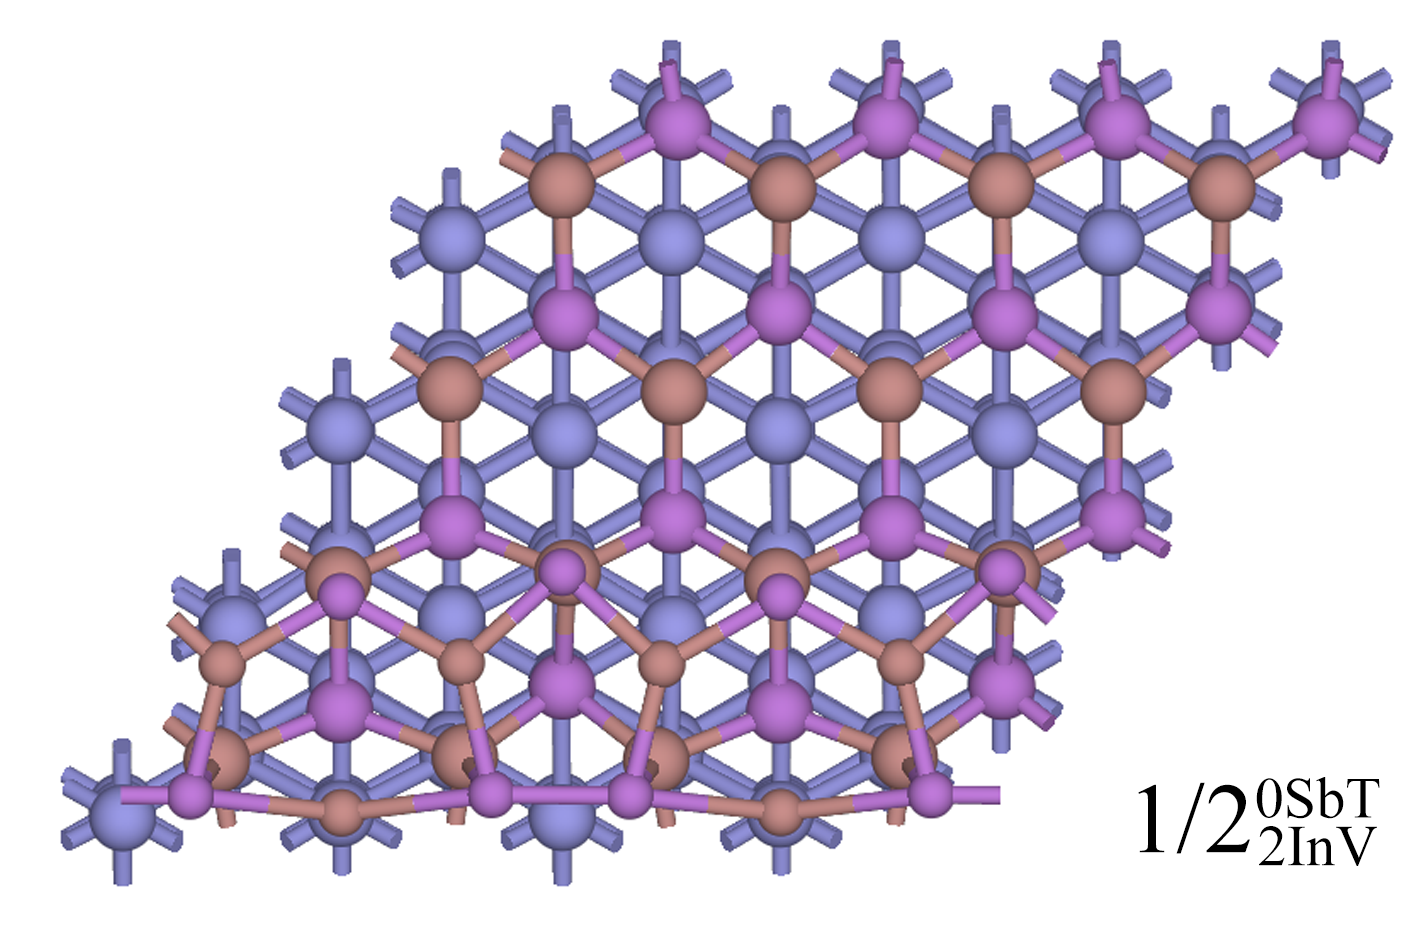
\includegraphics{pic/IS_structure_partical_1-2_2-0.png}
    }\\[-1ex]
    \subfloat[]{
        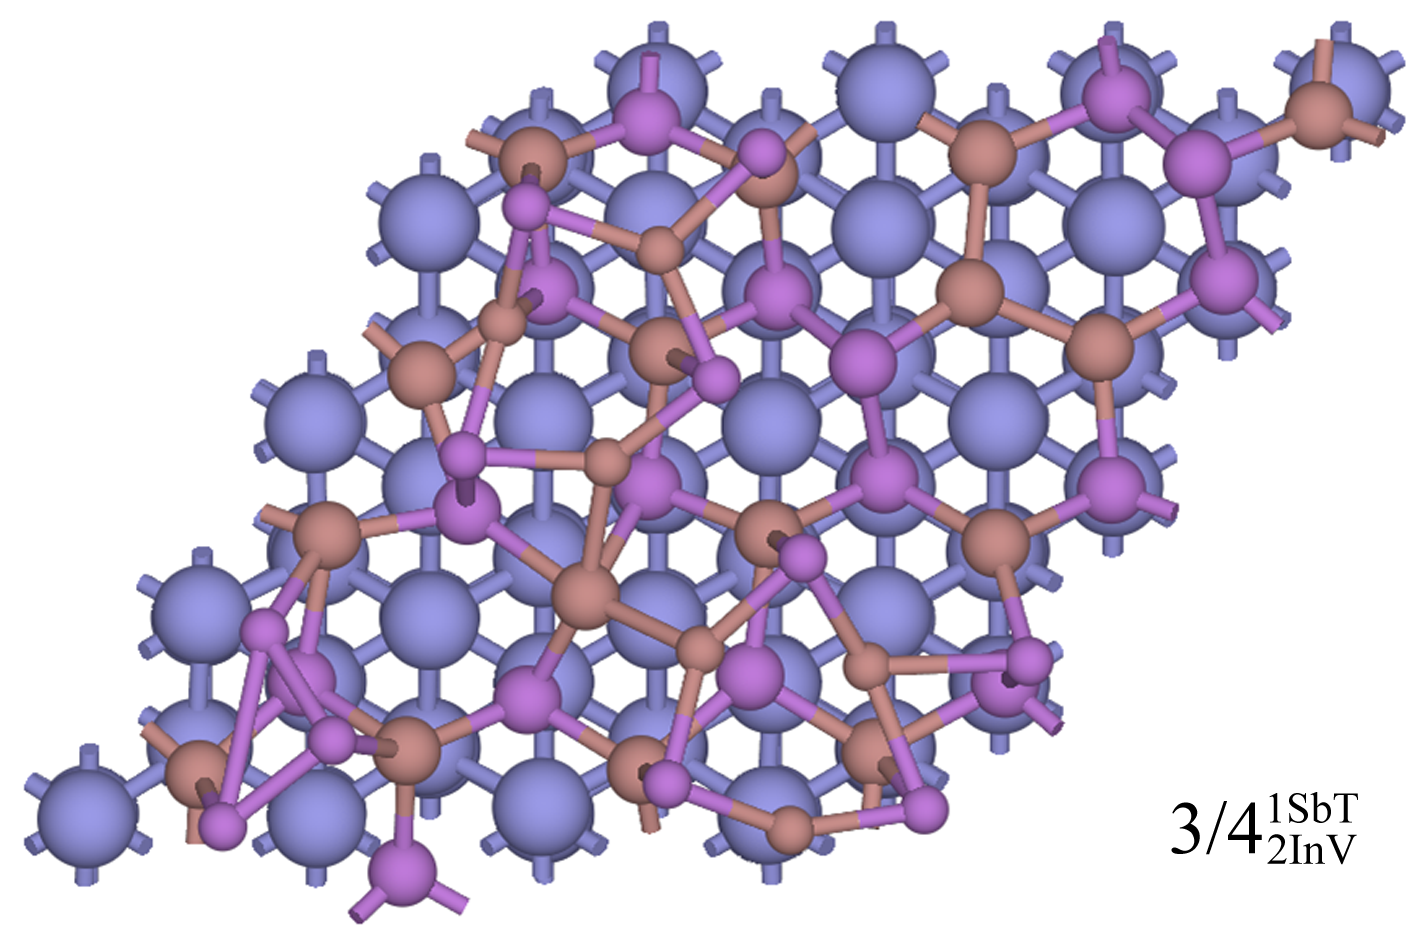
\includegraphics{pic/IS_structure_partical_3-4_2-1.png}
    }
    \subfloat[]{
        \includegraphics{pic/IS_structure_partical_3-4_0-3.png}
    }
\end{figure}

\begin{figure}
    \includegraphics{pic/IS_DFT_2LInSb_partPhase.png}
\end{figure}

\subsection{双层锑化铟的极性演化机理}

\begin{figure}
    \subfloat[]{
        \includegraphics{pic/IS_structure_slab_pseH_SbT.png}
    }\\[-0.5ex]
    \subfloat[]{
        \includegraphics{pic/IS_structure_slab_pseH_InP.png}
    }
\end{figure}

\begin{figure}
    \subfloat[]{
        \includegraphics[width=0.45\textwidth]{pic/IS_structure_cluster_2.png}
    }
    \subfloat[]{
        \includegraphics[width=0.45\textwidth]{pic/IS_structure_cluster_3.png}
    }\\[-0.5ex]
    \subfloat[]{
        \includegraphics[width=0.45\textwidth]{pic/IS_structure_cluster_7.png}
    }
    \subfloat[]{
        \includegraphics[width=0.45\textwidth]{pic/IS_structure_cluster_8.png}
    }
\end{figure}

\begin{figure}
    \includegraphics{pic/IS_DFT_surfaceE_InPSbP.png}
\end{figure}

\begin{figure}
    \includegraphics{pic/IS_DFT_PDOS-COHP.png}
\end{figure}

\begin{figure}
    \includegraphics{pic/IS_DFT_surfaceE_InVSbT.png}
\end{figure}
在赝氢饱和法中,具有 %//TODO

在四面体法中,%//TODO
\section{总结}